%\pdfoutput=1
% Uncomment line above if submitting to arXiv and using pdflatex
% ============================================================================
% Purpose: Template for LHCb documents
% Authors: Tomasz Skwarnicki, Roger Forty, Ulrik Egede, Patrick Koppenburg
% Created on: 2010-09-24
% ============================================================================
\documentclass[12pt,a4paper]{article}
%%\documentclass[12pt,letter]{article}
% For two column text, add "twocolumn" as an option to the document
% class. Also uncomment the two "onecolumn" and "twocolumn" lines
% around the title page below.

% Variables that controls behaviour
\usepackage{ifthen} % for conditional statements
\newboolean{pdflatex}
\setboolean{pdflatex}{true} % False for eps figures 

\newboolean{articletitles}
\setboolean{articletitles}{true} % False removes titles in references

\newboolean{uprightparticles}
\setboolean{uprightparticles}{true} % CHANGED

%\newboolean{inbibliography}
%\setboolean{inbibliography}{false} %True once you enter the bibliography

% Define titles and authors here. It will then be used both in metadata and in
% what is printed on the front page.
\def\paperauthors{LHCb collaboration} % Leave as is for PAPER, CONF and FIGURE
\def\paperasciititle{Template for writing LHCb papers} % Set ASCII title here !! MAKE sure it's only ASCII characters !! 
\def\papertitle{Template for writing \lhcb papers} % Latex formatted title
\def\paperkeywords{{High Energy Physics}, {LHCb}} % Comma separated list
%\def\papercopyright{CERN on behalf of the LHCb collaboration}
\def\papercopyright{\the\year\ CERN for the benefit of the LHCb collaboration} % new since 9/Apr/2018
\def\paperlicence{CC BY 4.0 licence}
\def\paperlicenceurl{https://creativecommons.org/licenses/by/4.0/}


%%%%%%%%%%%%%%%%%%%%%%%%%%%%%%%%%%%%%%%%%%%%%%%%%%%%%%%%%%%%%%%%%%%%%%
%                                                                    %
% !!!!!!!!!!!!!!!!!!! DO NOT EDIT THIS FILE !!!!!!!!!!!!!!!!!!!!!!!! %
%                                                                    %
% THE EB MAY OVERWRITE IT TO REFLECT LATEST CHANGES IN THE TEMPLATE  %
%                                                                    %
% You may define your own macros and packages in main.tex or add     %
% additional local files                                             %
%%%%%%%%%%%%%%%%%%%%%%%%%%%%%%%%%%%%%%%%%%%%%%%%%%%%%%%%%%%%%%%%%%%%%%
% THis file contains all the default packages and modifications for
% LHCb formatting

%% %%%%%%%%%%%%%%%%%%
%%  Page formatting
%% %%%%%%%%%%%%%%%%%%
%%\usepackage[margin=1in]{geometry}
\usepackage[top=1in, bottom=1.25in, left=1in, right=1in]{geometry}

% fallback for manual settings... uncomment if the geometry package is not available
%
%\voffset=-11mm
%\textheight=220mm
%\textwidth=160mm
%\oddsidemargin=0mm
%\evensidemargin=0mm

\columnsep=5mm
\addtolength{\belowcaptionskip}{0.5em}

\renewcommand{\textfraction}{0.01}
\renewcommand{\floatpagefraction}{0.8} % changed from 0.99
\renewcommand{\topfraction}{0.9}
\renewcommand{\bottomfraction}{0.9}

% Allow the page size to vary a bit ...
\raggedbottom
% To avoid Latex to be too fussy with line breaking ...
\sloppy

%% %%%%%%%%%%%%%%%%%%%%%%%
%% Packages to be used
%% %%%%%%%%%%%%%%%%%%%%%%% 
\usepackage{microtype}
\usepackage{lineno}  % for line numbering during review
\usepackage{xspace} % To avoid problems with missing or double spaces after
                    % predefined symbold
\usepackage{caption} %these three command get the figure and table captions automatically small
\renewcommand{\captionfont}{\small}
\renewcommand{\captionlabelfont}{\small}

%% Graphics
\usepackage{graphicx}  % to include figures (can also use other packages)
\usepackage{color}
\usepackage{colortbl}
\graphicspath{{./figs/}} % Make Latex search fig subdir for figures
% \DeclareGraphicsExtensions{.pdf,.PDF,.png,.PNG}   % not needed

%% Math
\usepackage{amsmath} % Adds a large collection of math symbols
\usepackage{amssymb}
\usepackage{amsfonts}
\usepackage{upgreek} % Adds in support for greek letters in roman typeset

%% fix to allow peaceful coexistence of line numbering and
%% mathematical objects
%% http://www.latex-community.org/forum/viewtopic.php?f=5&t=163
%%
\newcommand*\patchAmsMathEnvironmentForLineno[1]{%
\expandafter\let\csname old#1\expandafter\endcsname\csname #1\endcsname
\expandafter\let\csname oldend#1\expandafter\endcsname\csname
end#1\endcsname
 \renewenvironment{#1}%
   {\linenomath\csname old#1\endcsname}%
   {\csname oldend#1\endcsname\endlinenomath}%
}
\newcommand*\patchBothAmsMathEnvironmentsForLineno[1]{%
  \patchAmsMathEnvironmentForLineno{#1}%
  \patchAmsMathEnvironmentForLineno{#1*}%
}
\AtBeginDocument{%
\patchBothAmsMathEnvironmentsForLineno{equation}%
\patchBothAmsMathEnvironmentsForLineno{align}%
\patchBothAmsMathEnvironmentsForLineno{flalign}%
\patchBothAmsMathEnvironmentsForLineno{alignat}%
\patchBothAmsMathEnvironmentsForLineno{gather}%
\patchBothAmsMathEnvironmentsForLineno{multline}%
\patchBothAmsMathEnvironmentsForLineno{eqnarray}%
}

% Get hyperlinks to captions and in references.
% These do not work with revtex. Use "hypertext" as class option instead.

\usepackage{hyperxmp}

\usepackage[pdftex,
            pdfauthor={\paperauthors},
            pdftitle={\paperasciititle},
            pdfkeywords={\paperkeywords},
            pdfcopyright={Copyright (C) \papercopyright},
            pdflicenseurl={\paperlicenceurl}]{hyperref}
% if you have a mysterious compilation error at this line, check there are only ascii characters in \paperasciititle (main.tex)

% overleaf comments
\usepackage[colorinlistoftodos,textsize=scriptsize]{todonotes}

% get footnotes below floats
\usepackage[bottom,flushmargin,hang,multiple]{footmisc}

\usepackage[all]{hypcap} % Internal hyperlinks to floats.

%%%%%%%%%%%%%%%%%%%%%%%%%%%%%%%%%%%%%%%%%%%%%%%%%%%%%%%%%%%%%%%%%%%%%%%%
%%%                                                                    %
%%% !!!!!!!!!!!!!!!!!!! DO NOT EDIT THIS FILE !!!!!!!!!!!!!!!!!!!!!!!! %
%%%                                                                    %
%%% THE EB MAY OVERWRITE IT TO REFLECT LATEST CHANGES IN THE TEMPLATE  %
%%%                                                                    %
%%% You may define your own macros and packages in main.tex or add     %
%%% additional local files                                             %
%%%%%%%%%%%%%%%%%%%%%%%%%%%%%%%%%%%%%%%%%%%%%%%%%%%%%%%%%%%%%%%%%%%%%%%%
%%% ======================================================================
%%% Purpose: Standard LHCb aliases
%%% Author: Originally Ulrik Egede, adapted by Tomasz Skwarnicki for templates,
%%% rewritten by Chris Parkes
%%% Maintainer : Ulrik Egede (2010 - 2012)
%%% Maintainer : Rolf Oldeman (2012 - 2014)
%%% Maintainer : Patrick Koppenburg (2018--2020)
%%% =======================================================================
%%% To use this file outside the normal LHCb document environment, the
%%% following should be added in a preamble (before \begin{document}
%%%
%%%\usepackage{ifthen} 
%%%\newboolean{uprightparticles}
%%%\setboolean{uprightparticles}{false} %Set true for upright particle symbols
\usepackage{xspace} 
\usepackage{upgreek}


%%%%%%%%%%%%%%%%%%%%%%%%%%%%%%%%%%%%%%%%%%%%%%%%%%%%%%%%%%%%
%%%
%%% The following is to ensure that the template automatically can process
%%% this file.
%%%
%%% Add comments with at least three %%% preceding.
%%% Add new sections with one % preceding
%%% Add new subsections with two %% preceding
%%%
%%% For upper greek letters, Xires and Xiresbar will be the particles without the charge
%%% States with charge are called Xiz and Xim  
%%%
%%%%%%%%%%%%%%%%%%%%%%%%%%%%%%%%%%%%%%%%%%%%%%%%%%%%%%%%%%%%

%%%%%%%%%%%%%
% Experiments
%%%%%%%%%%%%%
\def\lhcb   {\mbox{LHCb}\xspace}
\def\atlas  {\mbox{ATLAS}\xspace}
\def\cms    {\mbox{CMS}\xspace}
\def\alice  {\mbox{ALICE}\xspace}
\def\babar  {\mbox{BaBar}\xspace}
\def\belle  {\mbox{Belle}\xspace}
\def\belletwo {\mbox{Belle~II}\xspace}
\def\besiii {\mbox{BESIII}\xspace}
\def\cleo   {\mbox{CLEO}\xspace}
\def\cdf    {\mbox{CDF}\xspace}
\def\dzero  {\mbox{D0}\xspace}
\def\aleph  {\mbox{ALEPH}\xspace}
\def\delphi {\mbox{DELPHI}\xspace}
\def\opal   {\mbox{OPAL}\xspace}
\def\lthree {\mbox{L3}\xspace}
\def\sld    {\mbox{SLD}\xspace}
%%%\def\argus  {\mbox{ARGUS}\xspace}
%%%\def\uaone  {\mbox{UA1}\xspace}
%%%\def\uatwo  {\mbox{UA2}\xspace}
%%%\def\ux85 {\mbox{UX85}\xspace}
\def\cern {\mbox{CERN}\xspace}
\def\lhc    {\mbox{LHC}\xspace}
\def\lep    {\mbox{LEP}\xspace}
\def\tevatron {Tevatron\xspace}
\def\bfactories {\mbox{\B Factories}\xspace}
\def\bfactory   {\mbox{\B Factory}\xspace}
\def\upgradeone {\mbox{Upgrade~I}\xspace}
\def\upgradetwo {\mbox{Upgrade~II}\xspace}

%% LHCb sub-detectors and sub-systems

%%%\def\pu     {PU\xspace}
\def\velo   {VELO\xspace}
\def\rich   {RICH\xspace}
\def\richone {RICH1\xspace}
\def\richtwo {RICH2\xspace}
\def\ttracker {TT\xspace}
\def\intr   {IT\xspace}
\def\st     {ST\xspace}
\def\ot     {OT\xspace}
\def\herschel {\mbox{\textsc{HeRSCheL}}\xspace}
%%%\def\Tone   {T1\xspace}
%%%\def\Ttwo   {T2\xspace}
%%%\def\Tthree {T3\xspace}
%%%\def\Mone   {M1\xspace}
%%%\def\Mtwo   {M2\xspace}
%%%\def\Mthree {M3\xspace}
%%%\def\Mfour  {M4\xspace}
%%%\def\Mfive  {M5\xspace}
\def\spd    {SPD\xspace}
\def\presh  {PS\xspace}
\def\ecal   {ECAL\xspace}
\def\hcal   {HCAL\xspace}
%%%\def\bcm    {BCM\xspace}
\def\MagUp {\mbox{\em Mag\kern -0.05em Up}\xspace}
\def\MagDown {\mbox{\em MagDown}\xspace}

\def\ode    {ODE\xspace}
\def\daq    {DAQ\xspace}
\def\tfc    {TFC\xspace}
\def\ecs    {ECS\xspace}
\def\lone   {L0\xspace}
\def\hlt    {HLT\xspace}
\def\hltone {HLT1\xspace}
\def\hlttwo {HLT2\xspace}

%%% Upright (not slanted) Particles

\ifthenelse{\boolean{uprightparticles}}%
{\def\Palpha      {\ensuremath{\upalpha}\xspace}
 \def\Pbeta       {\ensuremath{\upbeta}\xspace}
 \def\Pgamma      {\ensuremath{\upgamma}\xspace}                 
 \def\Pdelta      {\ensuremath{\updelta}\xspace}                 
 \def\Pepsilon    {\ensuremath{\upepsilon}\xspace}                 
 \def\Pvarepsilon {\ensuremath{\upvarepsilon}\xspace}                 
 \def\Pzeta       {\ensuremath{\upzeta}\xspace}                 
 \def\Peta        {\ensuremath{\upeta}\xspace}
 \def\Ptheta      {\ensuremath{\uptheta}\xspace}                 
 \def\Pvartheta   {\ensuremath{\upvartheta}\xspace}                 
 \def\Piota       {\ensuremath{\upiota}\xspace}                 
 \def\Pkappa      {\ensuremath{\upkappa}\xspace}                 
 \def\Plambda     {\ensuremath{\uplambda}\xspace}                 
 \def\Pmu         {\ensuremath{\upmu}\xspace}                 
 \def\Pnu         {\ensuremath{\upnu}\xspace}                 
 \def\Pxi         {\ensuremath{\upxi}\xspace}                 
 \def\Ppi         {\ensuremath{\uppi}\xspace}                 
 \def\Pvarpi      {\ensuremath{\upvarpi}\xspace}                 
 \def\Prho        {\ensuremath{\uprho}\xspace}                 
 \def\Pvarrho     {\ensuremath{\upvarrho}\xspace}                 
 \def\Ptau        {\ensuremath{\uptau}\xspace}                 
 \def\Pupsilon    {\ensuremath{\upupsilon}\xspace}                 
 \def\Pphi        {\ensuremath{\upphi}\xspace}                 
 \def\Pvarphi     {\ensuremath{\upvarphi}\xspace}                 
 \def\Pchi        {\ensuremath{\upchi}\xspace}                 
 \def\Ppsi        {\ensuremath{\uppsi}\xspace}                 
 \def\Pomega      {\ensuremath{\upomega}\xspace}                 

 \def\PDelta      {\ensuremath{\Delta}\xspace}                 
 \def\PXi         {\ensuremath{\Xi}\xspace}                 
 \def\PLambda     {\ensuremath{\Lambda}\xspace}                 
 \def\PSigma      {\ensuremath{\Sigma}\xspace}                 
 \def\POmega      {\ensuremath{\Omega}\xspace}                 
 \def\PUpsilon    {\ensuremath{\Upsilon}\xspace}
 \let\oldPi\Pi
 \def\PPi         {\ensuremath{\oldPi}\xspace}                 
               

 \def\PA      {\ensuremath{\mathrm{A}}\xspace}                 
 \def\PB      {\ensuremath{\mathrm{B}}\xspace}                 
 \def\PC      {\ensuremath{\mathrm{C}}\xspace}                 
 \def\PD      {\ensuremath{\mathrm{D}}\xspace}                 
 \def\PE      {\ensuremath{\mathrm{E}}\xspace}                 
 \def\PF      {\ensuremath{\mathrm{F}}\xspace}                 
 \def\PG      {\ensuremath{\mathrm{G}}\xspace}                 
 \def\PH      {\ensuremath{\mathrm{H}}\xspace}                 
 \def\PI      {\ensuremath{\mathrm{I}}\xspace}                 
 \def\PJ      {\ensuremath{\mathrm{J}}\xspace}                 
 \def\PK      {\ensuremath{\mathrm{K}}\xspace}                 
 \def\PL      {\ensuremath{\mathrm{L}}\xspace}                 
 \def\PM      {\ensuremath{\mathrm{M}}\xspace}                 
 \def\PN      {\ensuremath{\mathrm{N}}\xspace}                 
 \def\PO      {\ensuremath{\mathrm{O}}\xspace}                 
 \def\PP      {\ensuremath{\mathrm{P}}\xspace}                 
 \def\PQ      {\ensuremath{\mathrm{Q}}\xspace}                 
 \def\PR      {\ensuremath{\mathrm{R}}\xspace}                 
 \def\PS      {\ensuremath{\mathrm{S}}\xspace}                 
 \def\PT      {\ensuremath{\mathrm{T}}\xspace}                 
 \def\PU      {\ensuremath{\mathrm{U}}\xspace}                 
 \def\PV      {\ensuremath{\mathrm{V}}\xspace}                 
 \def\PW      {\ensuremath{\mathrm{W}}\xspace}                 
 \def\PX      {\ensuremath{\mathrm{X}}\xspace}                 
 \def\PY      {\ensuremath{\mathrm{Y}}\xspace}                 
 \def\PZ      {\ensuremath{\mathrm{Z}}\xspace}                 
 \def\Pa      {\ensuremath{\mathrm{a}}\xspace}                 
 \def\Pb      {\ensuremath{\mathrm{b}}\xspace}                 
 \def\Pc      {\ensuremath{\mathrm{c}}\xspace}                 
 \def\Pd      {\ensuremath{\mathrm{d}}\xspace}                 
 \def\Pe      {\ensuremath{\mathrm{e}}\xspace}                 
 \def\Pf      {\ensuremath{\mathrm{f}}\xspace}                 
 \def\Pg      {\ensuremath{\mathrm{g}}\xspace}                 
 \def\Ph      {\ensuremath{\mathrm{h}}\xspace}                 
 \def\Pi      {\ensuremath{\mathrm{i}}\xspace}                 
 \def\Pj      {\ensuremath{\mathrm{j}}\xspace}                 
 \def\Pk      {\ensuremath{\mathrm{k}}\xspace}                 
 \def\Pl      {\ensuremath{\mathrm{l}}\xspace}                 
 \def\Pm      {\ensuremath{\mathrm{m}}\xspace}                 
 \def\Pn      {\ensuremath{\mathrm{n}}\xspace}                 
 \def\Po      {\ensuremath{\mathrm{o}}\xspace}                 
 \def\Pp      {\ensuremath{\mathrm{p}}\xspace}                 
 \def\Pq      {\ensuremath{\mathrm{q}}\xspace}                 
 \def\Pr      {\ensuremath{\mathrm{r}}\xspace}                 
 \def\Ps      {\ensuremath{\mathrm{s}}\xspace}                 
 \def\Pt      {\ensuremath{\mathrm{t}}\xspace}                 
 \def\Pu      {\ensuremath{\mathrm{u}}\xspace}                 
 \def\Pv      {\ensuremath{\mathrm{v}}\xspace}                 
 \def\Pw      {\ensuremath{\mathrm{w}}\xspace}                 
 \def\Px      {\ensuremath{\mathrm{x}}\xspace}                 
 \def\Py      {\ensuremath{\mathrm{y}}\xspace}                 
 \def\Pz      {\ensuremath{\mathrm{z}}\xspace}                 
 \def\thebaroffset{0.0em}
}
{\def\Palpha      {\ensuremath{\alpha}\xspace}
 \def\Pbeta       {\ensuremath{\beta}\xspace}
 \def\Pgamma      {\ensuremath{\gamma}\xspace}                 
 \def\Pdelta      {\ensuremath{\delta}\xspace}                 
 \def\Pepsilon    {\ensuremath{\epsilon}\xspace}                 
 \def\Pvarepsilon {\ensuremath{\varepsilon}\xspace}                 
 \def\Pzeta       {\ensuremath{\zeta}\xspace}                 
 \def\Peta        {\ensuremath{\eta}\xspace}                 
 \def\Ptheta      {\ensuremath{\theta}\xspace}                 
 \def\Pvartheta   {\ensuremath{\vartheta}\xspace}                 
 \def\Piota       {\ensuremath{\iota}\xspace}                 
 \def\Pkappa      {\ensuremath{\kappa}\xspace}                 
 \def\Plambda     {\ensuremath{\lambda}\xspace}                 
 \def\Pmu         {\ensuremath{\mu}\xspace}                 
 \def\Pnu         {\ensuremath{\nu}\xspace}                 
 \def\Pxi         {\ensuremath{\xi}\xspace}                 
 \def\Ppi         {\ensuremath{\pi}\xspace}                 
 \def\Pvarpi      {\ensuremath{\varpi}\xspace}                 
 \def\Prho        {\ensuremath{\rho}\xspace}                 
 \def\Pvarrho     {\ensuremath{\varrho}\xspace}                 
 \def\Ptau        {\ensuremath{\tau}\xspace}                 
 \def\Pupsilon    {\ensuremath{\upsilon}\xspace}                 
 \def\Pphi        {\ensuremath{\phi}\xspace}                 
 \def\Pvarphi     {\ensuremath{\varphi}\xspace}                 
 \def\Pchi        {\ensuremath{\chi}\xspace}                 
 \def\Ppsi        {\ensuremath{\psi}\xspace}                 
 \def\Pomega      {\ensuremath{\omega}\xspace}                 
 \mathchardef\PDelta="7101
 \mathchardef\PXi="7104
 \mathchardef\PLambda="7103
 \mathchardef\PSigma="7106
 \mathchardef\POmega="710A
 \mathchardef\PUpsilon="7107
 \mathchardef\PPi="7105
 \def\PA      {\ensuremath{A}\xspace}                 
 \def\PB      {\ensuremath{B}\xspace}                 
 \def\PC      {\ensuremath{C}\xspace}                 
 \def\PD      {\ensuremath{D}\xspace}                 
 \def\PE      {\ensuremath{E}\xspace}                 
 \def\PF      {\ensuremath{F}\xspace}                 
 \def\PG      {\ensuremath{G}\xspace}                 
 \def\PH      {\ensuremath{H}\xspace}                 
 \def\PI      {\ensuremath{I}\xspace}                 
 \def\PJ      {\ensuremath{J}\xspace}                 
 \def\PK      {\ensuremath{K}\xspace}                 
 \def\PL      {\ensuremath{L}\xspace}                 
 \def\PM      {\ensuremath{M}\xspace}                 
 \def\PN      {\ensuremath{N}\xspace}                 
 \def\PO      {\ensuremath{O}\xspace}                 
 \def\PP      {\ensuremath{P}\xspace}                 
 \def\PQ      {\ensuremath{Q}\xspace}                 
 \def\PR      {\ensuremath{R}\xspace}                 
 \def\PS      {\ensuremath{S}\xspace}                 
 \def\PT      {\ensuremath{T}\xspace}                 
 \def\PU      {\ensuremath{U}\xspace}                 
 \def\PV      {\ensuremath{V}\xspace}                 
 \def\PW      {\ensuremath{W}\xspace}                 
 \def\PX      {\ensuremath{X}\xspace}                 
 \def\PY      {\ensuremath{Y}\xspace}                 
 \def\PZ      {\ensuremath{Z}\xspace}                 
 \def\Pa      {\ensuremath{a}\xspace}                 
 \def\Pb      {\ensuremath{b}\xspace}                 
 \def\Pc      {\ensuremath{c}\xspace}                 
 \def\Pd      {\ensuremath{d}\xspace}                 
 \def\Pe      {\ensuremath{e}\xspace}                 
 \def\Pf      {\ensuremath{f}\xspace}                 
 \def\Pg      {\ensuremath{g}\xspace}                 
 \def\Ph      {\ensuremath{h}\xspace}                 
 \def\Pi      {\ensuremath{i}\xspace}                 
 \def\Pj      {\ensuremath{j}\xspace}                 
 \def\Pk      {\ensuremath{k}\xspace}                 
 \def\Pl      {\ensuremath{l}\xspace}                 
 \def\Pm      {\ensuremath{m}\xspace}                 
 \def\Pn      {\ensuremath{n}\xspace}                 
 \def\Po      {\ensuremath{o}\xspace}                 
 \def\Pp      {\ensuremath{p}\xspace}                 
 \def\Pq      {\ensuremath{q}\xspace}                 
 \def\Pr      {\ensuremath{r}\xspace}                 
 \def\Ps      {\ensuremath{s}\xspace}                 
 \def\Pt      {\ensuremath{t}\xspace}                 
 \def\Pu      {\ensuremath{u}\xspace}                 
 \def\Pv      {\ensuremath{v}\xspace}                 
 \def\Pw      {\ensuremath{w}\xspace}                 
 \def\Px      {\ensuremath{x}\xspace}                 
 \def\Py      {\ensuremath{y}\xspace}                 
 \def\Pz      {\ensuremath{z}\xspace}
 \def\thebaroffset{0.18em}
}
\newcommand{\offsetoverline}[2][\thebaroffset]{\kern #1\overline{\kern -#1 #2}}%

%%%%%%%%%%%%%%%%%%%%%%%%%%%%%%%%%%%%%%%%%%%%%%%
% Particles
\makeatletter
\ifcase \@ptsize \relax% 10pt
  \newcommand{\miniscule}{\@setfontsize\miniscule{4}{5}}% \tiny: 5/6
\or% 11pt
  \newcommand{\miniscule}{\@setfontsize\miniscule{5}{6}}% \tiny: 6/7
\or% 12pt
  \newcommand{\miniscule}{\@setfontsize\miniscule{5}{6}}% \tiny: 6/7
\fi
\makeatother


\DeclareRobustCommand{\optbar}[1]{\shortstack{{\miniscule (\rule[.5ex]{1.25em}{.18mm})}
  \\ [-.7ex] $#1$}}


%% Leptons

\let\emi\en
\def\electron   {{\ensuremath{\Pe}}\xspace}
\def\en         {{\ensuremath{\Pe^-}}\xspace}   % electron negative (\em is taken)
\def\ep         {{\ensuremath{\Pe^+}}\xspace}
\def\epm        {{\ensuremath{\Pe^\pm}}\xspace} 
\def\emp        {{\ensuremath{\Pe^\mp}}\xspace} 
\def\epem       {{\ensuremath{\Pe^+\Pe^-}}\xspace}
%%%\def\ee         {\ensuremath{\Pe^-\Pe^-}\xspace}

\def\muon       {{\ensuremath{\Pmu}}\xspace}
\def\mup        {{\ensuremath{\Pmu^+}}\xspace}
\def\mun        {{\ensuremath{\Pmu^-}}\xspace} % muon negative (\mum is taken)
\def\mupm       {{\ensuremath{\Pmu^\pm}}\xspace} 
\def\mump       {{\ensuremath{\Pmu^\mp}}\xspace} 
\def\mumu       {{\ensuremath{\Pmu^+\Pmu^-}}\xspace}

\def\tauon      {{\ensuremath{\Ptau}}\xspace}
\def\taup       {{\ensuremath{\Ptau^+}}\xspace}
\def\taum       {{\ensuremath{\Ptau^-}}\xspace}
\def\taupm      {{\ensuremath{\Ptau^\pm}}\xspace}
\def\taump      {{\ensuremath{\Ptau^\mp}}\xspace}
\def\tautau     {{\ensuremath{\Ptau^+\Ptau^-}}\xspace}

\def\lepton     {{\ensuremath{\ell}}\xspace}
\def\ellm       {{\ensuremath{\ell^-}}\xspace}
\def\ellp       {{\ensuremath{\ell^+}}\xspace}
\def\ellpm      {{\ensuremath{\ell^\pm}}\xspace}
\def\ellmp      {{\ensuremath{\ell^\mp}}\xspace}
\def\ellell     {\ensuremath{\ell^+ \ell^-}\xspace}

\def\neu        {{\ensuremath{\Pnu}}\xspace}
\def\neub       {{\ensuremath{\overline{\Pnu}}}\xspace}
%%%\def\nuenueb    {\ensuremath{\neu\neub}\xspace}
\def\neue       {{\ensuremath{\neu_e}}\xspace}
\def\neueb      {{\ensuremath{\neub_e}}\xspace}
%%%\def\neueneueb  {\ensuremath{\neue\neueb}\xspace}
\def\neum       {{\ensuremath{\neu_\mu}}\xspace}
\def\neumb      {{\ensuremath{\neub_\mu}}\xspace}
%%%\def\neumneumb  {\ensuremath{\neum\neumb}\xspace}
\def\neut       {{\ensuremath{\neu_\tau}}\xspace}
\def\neutb      {{\ensuremath{\neub_\tau}}\xspace}
%%%\def\neutneutb  {\ensuremath{\neut\neutb}\xspace}
\def\neul       {{\ensuremath{\neu_\ell}}\xspace}
\def\neulb      {{\ensuremath{\neub_\ell}}\xspace}
%%%\def\neulneulb  {\ensuremath{\neul\neulb}\xspace}

%% Gauge bosons and scalars

\def\g      {{\ensuremath{\Pgamma}}\xspace}
\def\H      {{\ensuremath{\PH^0}}\xspace}
\def\Hp     {{\ensuremath{\PH^+}}\xspace}
\def\Hm     {{\ensuremath{\PH^-}}\xspace}
\def\Hpm    {{\ensuremath{\PH^\pm}}\xspace}
\def\W      {{\ensuremath{\PW}}\xspace}
\def\Wp     {{\ensuremath{\PW^+}}\xspace}
\def\Wm     {{\ensuremath{\PW^-}}\xspace}
\def\Wpm    {{\ensuremath{\PW^\pm}}\xspace}
\def\Z      {{\ensuremath{\PZ}}\xspace}

%% Quarks

\def\quark     {{\ensuremath{\Pq}}\xspace}
\def\quarkbar  {{\ensuremath{\overline \quark}}\xspace}
\def\qqbar     {{\ensuremath{\quark\quarkbar}}\xspace}
\def\uquark    {{\ensuremath{\Pu}}\xspace}
\def\uquarkbar {{\ensuremath{\overline \uquark}}\xspace}
\def\uubar     {{\ensuremath{\uquark\uquarkbar}}\xspace}
\def\dquark    {{\ensuremath{\Pd}}\xspace}
\def\dquarkbar {{\ensuremath{\overline \dquark}}\xspace}
\def\ddbar     {{\ensuremath{\dquark\dquarkbar}}\xspace}
\def\squark    {{\ensuremath{\Ps}}\xspace}
\def\squarkbar {{\ensuremath{\overline \squark}}\xspace}
\def\ssbar     {{\ensuremath{\squark\squarkbar}}\xspace}
\def\cquark    {{\ensuremath{\Pc}}\xspace}
\def\cquarkbar {{\ensuremath{\overline \cquark}}\xspace}
\def\ccbar     {{\ensuremath{\cquark\cquarkbar}}\xspace}
\def\bquark    {{\ensuremath{\Pb}}\xspace}
\def\bquarkbar {{\ensuremath{\overline \bquark}}\xspace}
\def\bbbar     {{\ensuremath{\bquark\bquarkbar}}\xspace}
\def\tquark    {{\ensuremath{\Pt}}\xspace}
\def\tquarkbar {{\ensuremath{\overline \tquark}}\xspace}
\def\ttbar     {{\ensuremath{\tquark\tquarkbar}}\xspace}

%% Light mesons

\def\hadron {{\ensuremath{\Ph}}\xspace}
\def\pion   {{\ensuremath{\Ppi}}\xspace}
\def\piz    {{\ensuremath{\pion^0}}\xspace}
\def\pip    {{\ensuremath{\pion^+}}\xspace}
\def\pim    {{\ensuremath{\pion^-}}\xspace}
\def\pipm   {{\ensuremath{\pion^\pm}}\xspace}
\def\pimp   {{\ensuremath{\pion^\mp}}\xspace}

\def\rhomeson {{\ensuremath{\Prho}}\xspace}
\def\rhoz     {{\ensuremath{\rhomeson^0}}\xspace}
\def\rhop     {{\ensuremath{\rhomeson^+}}\xspace}
\def\rhom     {{\ensuremath{\rhomeson^-}}\xspace}
\def\rhopm    {{\ensuremath{\rhomeson^\pm}}\xspace}
\def\rhomp    {{\ensuremath{\rhomeson^\mp}}\xspace}

\def\kaon    {{\ensuremath{\PK}}\xspace}
%%% do NOT use ensuremath here, and keep indent
\def\Kbar    {{\ensuremath{\offsetoverline{\PK}}}\xspace}
\def\Kb      {{\ensuremath{\Kbar}}\xspace}
\def\KorKbar {\kern \thebaroffset\optbar{\kern -\thebaroffset \PK}{}\xspace}
\def\Kz      {{\ensuremath{\kaon^0}}\xspace}
\def\Kzb     {{\ensuremath{\Kbar{}^0}}\xspace}
\def\Kp      {{\ensuremath{\kaon^+}}\xspace}
\def\Km      {{\ensuremath{\kaon^-}}\xspace}
\def\Kpm     {{\ensuremath{\kaon^\pm}}\xspace}
\def\Kmp     {{\ensuremath{\kaon^\mp}}\xspace}
\def\KS      {{\ensuremath{\kaon^0_{\mathrm{S}}}}\xspace}
\def\Vzero   {{\ensuremath{V^0}}\xspace}
\def\KL      {{\ensuremath{\kaon^0_{\mathrm{L}}}}\xspace}
\def\Kstarz  {{\ensuremath{\kaon^{*0}}}\xspace}
\def\Kstarzb {{\ensuremath{\Kbar{}^{*0}}}\xspace}
\def\Kstar   {{\ensuremath{\kaon^*}}\xspace}
\def\Kstarb  {{\ensuremath{\Kbar{}^*}}\xspace}
\def\Kstarp  {{\ensuremath{\kaon^{*+}}}\xspace}
\def\Kstarm  {{\ensuremath{\kaon^{*-}}}\xspace}
\def\Kstarpm {{\ensuremath{\kaon^{*\pm}}}\xspace}
\def\Kstarmp {{\ensuremath{\kaon^{*\mp}}}\xspace}
\def\KorKbarz {\ensuremath{\KorKbar^0}\xspace}

\newcommand{\etaz}{\ensuremath{\Peta}\xspace}
\newcommand{\etapr}{\ensuremath{\Peta^{\prime}}\xspace}
\newcommand{\phiz}{\ensuremath{\Pphi}\xspace}
\newcommand{\omegaz}{\ensuremath{\Pomega}\xspace}

%% Charmed mesons

%%% do NOT use ensuremath here (and keep indent)
\def\Dbar    {{\ensuremath{\offsetoverline{\PD}}}\xspace}
\def\D       {{\ensuremath{\PD}}\xspace}
\def\Db      {{\ensuremath{\Dbar}}\xspace}
\def\DorDbar {\kern \thebaroffset\optbar{\kern -\thebaroffset \PD}\xspace}
\def\Dz      {{\ensuremath{\D^0}}\xspace}
\def\Dzb     {{\ensuremath{\Dbar{}^0}}\xspace}
\def\Dp      {{\ensuremath{\D^+}}\xspace}
\def\Dm      {{\ensuremath{\D^-}}\xspace}
\def\Dpm     {{\ensuremath{\D^\pm}}\xspace}
\def\Dmp     {{\ensuremath{\D^\mp}}\xspace}
\def\DpDm    {\ensuremath{\Dp {\kern -0.16em \Dm}}\xspace}
\def\Dstar   {{\ensuremath{\D^*}}\xspace}
\def\Dstarb  {{\ensuremath{\Dbar{}^*}}\xspace}
\def\Dstarz  {{\ensuremath{\D^{*0}}}\xspace}
\def\Dstarzb {{\ensuremath{\Dbar{}^{*0}}}\xspace}
\def\theDstarz{{\ensuremath{\D^{*}(2007)^{0}}}\xspace}
\def\theDstarzb{{\ensuremath{\Dbar^{*}(2007)^{0}}}\xspace}
\def\Dstarp  {{\ensuremath{\D^{*+}}}\xspace}
\def\Dstarm  {{\ensuremath{\D^{*-}}}\xspace}
\def\Dstarpm {{\ensuremath{\D^{*\pm}}}\xspace}
\def\Dstarmp {{\ensuremath{\D^{*\mp}}}\xspace}
\def\theDstarp{{\ensuremath{\D^{*}(2010)^{+}}}\xspace}
\def\theDstarm{{\ensuremath{\D^{*}(2010)^{-}}}\xspace}
\def\theDstarpm{{\ensuremath{\D^{*}(2010)^{\pm}}}\xspace}
\def\theDstarmp{{\ensuremath{\D^{*}(2010)^{\mp}}}\xspace}
\def\Ds      {{\ensuremath{\D^+_\squark}}\xspace}
\def\Dsp     {{\ensuremath{\D^+_\squark}}\xspace}
\def\Dsm     {{\ensuremath{\D^-_\squark}}\xspace}
\def\Dspm    {{\ensuremath{\D^{\pm}_\squark}}\xspace}
\def\Dsmp    {{\ensuremath{\D^{\mp}_\squark}}\xspace}
\def\Dss     {{\ensuremath{\D^{*+}_\squark}}\xspace}
\def\Dssp    {{\ensuremath{\D^{*+}_\squark}}\xspace}
\def\Dssm    {{\ensuremath{\D^{*-}_\squark}}\xspace}
\def\Dsspm   {{\ensuremath{\D^{*\pm}_\squark}}\xspace}
\def\Dssmp   {{\ensuremath{\D^{*\mp}_\squark}}\xspace}
\def\DporDsp {{\ensuremath{\D_{(\squark)}^+}}\xspace}
\def\DmorDsm {{\ensuremath{\D{}_{(\squark)}^-}}\xspace}
\def\DpmorDspm {{\ensuremath{\D{}_{(\squark)}^\pm}}\xspace}

%% Beauty mesons
\def\B       {{\ensuremath{\PB}}\xspace}
\def\Bbar    {{\ensuremath{\offsetoverline{\PB}}}\xspace}
\def\Bb      {{\ensuremath{\Bbar}}\xspace}
\def\BorBbar {\kern \thebaroffset\optbar{\kern -\thebaroffset \PB}\xspace}
\def\Bz      {{\ensuremath{\B^0}}\xspace}
\def\Bzb     {{\ensuremath{\Bbar{}^0}}\xspace}
\def\Bd      {{\ensuremath{\B^0}}\xspace}
\def\Bdb     {{\ensuremath{\Bbar{}^0}}\xspace}
\def\BdorBdbar {\kern \thebaroffset\optbar{\kern -\thebaroffset \Bd}\xspace}
\def\Bu      {{\ensuremath{\B^+}}\xspace}
\def\Bub     {{\ensuremath{\B^-}}\xspace}
\def\Bp      {{\ensuremath{\Bu}}\xspace}
\def\Bm      {{\ensuremath{\Bub}}\xspace}
\def\Bpm     {{\ensuremath{\B^\pm}}\xspace}
\def\Bmp     {{\ensuremath{\B^\mp}}\xspace}
\def\Bs      {{\ensuremath{\B^0_\squark}}\xspace}
\def\Bsb     {{\ensuremath{\Bbar{}^0_\squark}}\xspace}
\def\BsorBsbar {\kern \thebaroffset\optbar{\kern -\thebaroffset \Bs}\xspace}
\def\Bc      {{\ensuremath{\B_\cquark^+}}\xspace}
\def\Bcp     {{\ensuremath{\B_\cquark^+}}\xspace}
\def\Bcm     {{\ensuremath{\B_\cquark^-}}\xspace}
\def\Bcpm    {{\ensuremath{\B_\cquark^\pm}}\xspace}
\def\Bds     {{\ensuremath{\B_{(\squark)}^0}}\xspace}
\def\Bdsb    {{\ensuremath{\Bbar{}_{(\squark)}^0}}\xspace}
\def\BdorBs  {\Bds}
\def\BdorBsbar  {\Bdsb}

%% Onia

\def\jpsi     {{\ensuremath{{\PJ\mskip -3mu/\mskip -2mu\Ppsi}}}\xspace}
\def\psitwos  {{\ensuremath{\Ppsi{(2S)}}}\xspace}
\def\psiprpr  {{\ensuremath{\Ppsi(3770)}}\xspace}
\def\etac     {{\ensuremath{\Peta_\cquark}}\xspace}
\def\psires  {{\ensuremath{\Ppsi}}\xspace}
\def\chic     {{\ensuremath{\Pchi_\cquark}}\xspace}
\def\chiczero {{\ensuremath{\Pchi_{\cquark 0}}}\xspace}
\def\chicone  {{\ensuremath{\Pchi_{\cquark 1}}}\xspace}
\def\chictwo  {{\ensuremath{\Pchi_{\cquark 2}}}\xspace}
\def\chicJ    {{\ensuremath{\Pchi_{\cquark J}}}\xspace}
\def\Upsilonres  {{\ensuremath{\PUpsilon}}\xspace}
\def\Y#1S{\ensuremath{\PUpsilon{(#1S)}}\xspace}
\def\OneS  {{\Y1S}\xspace}
\def\TwoS  {{\Y2S}\xspace}
\def\ThreeS{{\Y3S}\xspace}
\def\FourS {{\Y4S}\xspace}
\def\FiveS {{\Y5S}\xspace}
\def\chib     {{\ensuremath{\Pchi_{b}}}\xspace}
\def\chibzero {{\ensuremath{\Pchi_{\bquark 0}}}\xspace}
\def\chibone  {{\ensuremath{\Pchi_{\bquark 1}}}\xspace}
\def\chibtwo  {{\ensuremath{\Pchi_{\bquark 2}}}\xspace}
\def\chibJ    {{\ensuremath{\Pchi_{\bquark J}}}\xspace}
\def\theX     {{\ensuremath{\Pchi_{c1}(3872)}}\xspace}

%% Light Baryons

\def\proton      {{\ensuremath{\Pp}}\xspace}
\def\antiproton  {{\ensuremath{\overline \proton}}\xspace}
\def\neutron     {{\ensuremath{\Pn}}\xspace}
\def\antineutron {{\ensuremath{\overline \neutron}}\xspace}
\def\Deltares    {{\ensuremath{\PDelta}}\xspace}
\def\Deltaresbar {{\ensuremath{\overline \Deltares}}\xspace}
%%% uds singlet
\def\Lz          {{\ensuremath{\PLambda}}\xspace}
\def\Lbar        {{\ensuremath{\offsetoverline{\PLambda}}}\xspace}
\def\LorLbar     {\kern \thebaroffset\optbar{\kern -\thebaroffset \PLambda}\xspace}
\def\Lambdares   {{\ensuremath{\PLambda}}\xspace}
\def\Lambdaresbar{{\ensuremath{\Lbar}}\xspace}
%%% uus, uds, dds
\def\Sigmares    {{\ensuremath{\PSigma}}\xspace}
\def\Sigmaz      {{\ensuremath{\Sigmares{}^0}}\xspace}
\def\Sigmap      {{\ensuremath{\Sigmares{}^+}}\xspace}
\def\Sigmam      {{\ensuremath{\Sigmares{}^-}}\xspace}
\def\Sigmaresbar {{\ensuremath{\offsetoverline{\Sigmares}}}\xspace}
\def\Sigmabarz   {{\ensuremath{\Sigmaresbar{}^0}}\xspace}
\def\Sigmabarp   {{\ensuremath{\Sigmaresbar{}^+}}\xspace}
\def\Sigmabarm   {{\ensuremath{\Sigmaresbar{}^-}}\xspace}
%%%  uss, dss
\def\Xires       {{\ensuremath{\PXi}}\xspace}
\def\Xiz         {{\ensuremath{\Xires^0}}\xspace}
\def\Xim         {{\ensuremath{\Xires^-}}\xspace}
\def\Xiresbar       {{\ensuremath{\offsetoverline{\Xires}}}\xspace}
\def\Xibarz      {{\ensuremath{\Xiresbar^0}}\xspace}
\def\Xibarp      {{\ensuremath{\Xiresbar^+}}\xspace}
%%%  sss
\def\Omegares    {{\ensuremath{\POmega}}\xspace}
\def\Omegaresbar {{\ensuremath{\offsetoverline{\POmega}}}\xspace}
\def\Omegam      {{\ensuremath{\Omegares^-}}\xspace}
\def\Omegabarp   {{\ensuremath{\Omegaresbar^+}}\xspace}

%% Charmed Baryons
\def\Lc          {{\ensuremath{\Lz^+_\cquark}}\xspace}
\def\Lcbar       {{\ensuremath{\Lbar{}^-_\cquark}}\xspace}
\def\Xic         {{\ensuremath{\Xires_\cquark}}\xspace}
\def\Xicz        {{\ensuremath{\Xires^0_\cquark}}\xspace}
\def\Xicp        {{\ensuremath{\Xires^+_\cquark}}\xspace}
\def\Xicbar      {{\ensuremath{\Xiresbar{}_\cquark}}\xspace}
\def\Xicbarz     {{\ensuremath{\Xiresbar{}_\cquark^0}}\xspace}
\def\Xicbarm     {{\ensuremath{\Xiresbar{}_\cquark^-}}\xspace}
\def\Omegac      {{\ensuremath{\Omegares^0_\cquark}}\xspace}
\def\Omegacbar   {{\ensuremath{\Omegaresbar{}_\cquark^0}}\xspace}
\def\Xicc        {{\ensuremath{\Xires_{\cquark\cquark}}}\xspace}
\def\Xiccbar     {{\ensuremath{\Xiresbar{}_{\cquark\cquark}}}\xspace}
\def\Xiccp       {{\ensuremath{\Xires^+_{\cquark\cquark}}}\xspace}
\def\Xiccpp      {{\ensuremath{\Xires^{++}_{\cquark\cquark}}}\xspace}
\def\Xiccbarm    {{\ensuremath{\Xiresbar{}_{\cquark\cquark}^-}}\xspace}
\def\Xiccbarmm   {{\ensuremath{\Xiresbar{}_{\cquark\cquark}^{--}}}\xspace}
\def\Omegacc     {{\ensuremath{\Omegares^+_{\cquark\cquark}}}\xspace}
\def\Omegaccbar  {{\ensuremath{\Omegaresbar{}_{\cquark\cquark}^-}}\xspace}
\def\Omegaccc    {{\ensuremath{\Omegares^{++}_{\cquark\cquark\cquark}}}\xspace}
\def\Omegacccbar {{\ensuremath{\Omegaresbar{}_{\cquark\cquark\cquark}^{--}}}\xspace}
%% Beauty Baryons

\def\Lb           {{\ensuremath{\Lz^0_\bquark}}\xspace}
\def\Lbbar        {{\ensuremath{\Lbar{}^0_\bquark}}\xspace}
\def\Sigmab       {{\ensuremath{\Sigmares_\bquark}}\xspace}
\def\Sigmabp      {{\ensuremath{\Sigmares_\bquark^+}}\xspace}
\def\Sigmabz      {{\ensuremath{\Sigmares_\bquark^0}}\xspace}
\def\Sigmabm      {{\ensuremath{\Sigmares_\bquark^-}}\xspace}
\def\Sigmabpm     {{\ensuremath{\Sigmares_\bquark^\pm}}\xspace}
\def\Sigmabbar    {{\ensuremath{\Sigmaresbar_\bquark}}\xspace}
\def\Sigmabbarp   {{\ensuremath{\Sigmaresbar_\bquark^+}}\xspace}
\def\Sigmabbarz   {{\ensuremath{\Sigmaresbar_\bquark^0}}\xspace}
\def\Sigmabbarm   {{\ensuremath{\Sigmaresbar_\bquark^-}}\xspace}
\def\Sigmabbarpm  {{\ensuremath{\Sigmaresbar_\bquark^-}}\xspace}
\def\Xib          {{\ensuremath{\Xires_\bquark}}\xspace}
\def\Xibz         {{\ensuremath{\Xires^0_\bquark}}\xspace}
\def\Xibm         {{\ensuremath{\Xires^-_\bquark}}\xspace}
\def\Xibbar       {{\ensuremath{\Xiresbar{}_\bquark}}\xspace}
\def\Xibbarz      {{\ensuremath{\Xiresbar{}_\bquark^0}}\xspace}
\def\Xibbarp      {{\ensuremath{\Xiresbar{}_\bquark^+}}\xspace}
\def\Omegab       {{\ensuremath{\Omegares^-_\bquark}}\xspace}
\def\Omegabbar    {{\ensuremath{\Omegaresbar{}_\bquark^+}}\xspace}

%%%%%%%%%%%%%%%%%%
% Physics symbols
%%%%%%%%%%%%%%%%%

%% Decays
\def\BF         {{\ensuremath{\mathcal{B}}}\xspace}
\def\BR         {\BF}
\def\BRvis      {{\ensuremath{\BR_{\mathrm{{vis}}}}}}
\newcommand{\decay}[2]{\ensuremath{#1\!\to #2}\xspace} 
\def\ra                 {\ensuremath{\rightarrow}\xspace}
\def\to                 {\ensuremath{\rightarrow}\xspace}

%% Lifetimes
\newcommand{\tauBs}{{\ensuremath{\tau_{\Bs}}}\xspace}
\newcommand{\tauBd}{{\ensuremath{\tau_{\Bd}}}\xspace}
\newcommand{\tauBz}{{\ensuremath{\tau_{\Bz}}}\xspace}
\newcommand{\tauBu}{{\ensuremath{\tau_{\Bp}}}\xspace}
\newcommand{\tauDp}{{\ensuremath{\tau_{\Dp}}}\xspace}
\newcommand{\tauDz}{{\ensuremath{\tau_{\Dz}}}\xspace}
\newcommand{\tauL}{{\ensuremath{\tau_{\mathrm{ L}}}}\xspace}
\newcommand{\tauH}{{\ensuremath{\tau_{\mathrm{ H}}}}\xspace}

%% Masses
\newcommand{\mBd}{{\ensuremath{m_{\Bd}}}\xspace}
\newcommand{\mBp}{{\ensuremath{m_{\Bp}}}\xspace}
\newcommand{\mBs}{{\ensuremath{m_{\Bs}}}\xspace}
\newcommand{\mBc}{{\ensuremath{m_{\Bc}}}\xspace}
\newcommand{\mLb}{{\ensuremath{m_{\Lb}}}\xspace}

%% EW theory, groups
\def\grpsuthree {{\ensuremath{\mathrm{SU}(3)}}\xspace}
\def\grpsutw    {{\ensuremath{\mathrm{SU}(2)}}\xspace}
\def\grpuone    {{\ensuremath{\mathrm{U}(1)}}\xspace}

\def\ssqtw   {{\ensuremath{\sin^{2}\!\theta_{\mathrm{W}}}}\xspace}
\def\csqtw   {{\ensuremath{\cos^{2}\!\theta_{\mathrm{W}}}}\xspace}
\def\stw     {{\ensuremath{\sin\theta_{\mathrm{W}}}}\xspace}
\def\ctw     {{\ensuremath{\cos\theta_{\mathrm{W}}}}\xspace}
\def\ssqtwef {{\ensuremath{{\sin}^{2}\theta_{\mathrm{W}}^{\mathrm{eff}}}}\xspace}
\def\csqtwef {{\ensuremath{{\cos}^{2}\theta_{\mathrm{W}}^{\mathrm{eff}}}}\xspace}
\def\stwef   {{\ensuremath{\sin\theta_{\mathrm{W}}^{\mathrm{eff}}}}\xspace}
\def\ctwef   {{\ensuremath{\cos\theta_{\mathrm{W}}^{\mathrm{eff}}}}\xspace}
\def\gv      {{\ensuremath{g_{\mbox{\tiny V}}}}\xspace}
\def\ga      {{\ensuremath{g_{\mbox{\tiny A}}}}\xspace}

\def\order   {{\ensuremath{\mathcal{O}}}\xspace}
\def\ordalph {{\ensuremath{\mathcal{O}(\alpha)}}\xspace}
\def\ordalsq {{\ensuremath{\mathcal{O}(\alpha^{2})}}\xspace}
\def\ordalcb {{\ensuremath{\mathcal{O}(\alpha^{3})}}\xspace}

%% QCD parameters
\newcommand{\as}{{\ensuremath{\alpha_s}}\xspace}
\newcommand{\MSb}{{\ensuremath{\overline{\mathrm{MS}}}}\xspace}
\newcommand{\lqcd}{{\ensuremath{\Lambda_{\mathrm{QCD}}}}\xspace}
\def\qsq       {{\ensuremath{q^2}}\xspace}

%% CKM, \boldmath \CP violation

\def\eps   {{\ensuremath{\varepsilon}}\xspace}
\def\epsK  {{\ensuremath{\varepsilon_K}}\xspace}
\def\epsB  {{\ensuremath{\varepsilon_B}}\xspace}
\def\epsp  {{\ensuremath{\varepsilon^\prime_K}}\xspace}

\def\CP                {{\ensuremath{C\!P}}\xspace}
\def\CPT               {{\ensuremath{C\!PT}}\xspace}
\def\T                 {{\ensuremath{T}}\xspace}

\def\rhobar {{\ensuremath{\overline \rho}}\xspace}
\def\etabar {{\ensuremath{\overline \eta}}\xspace}

\def\Vud  {{\ensuremath{V_{\uquark\dquark}^{\phantom{\ast}}}}\xspace}
\def\Vcd  {{\ensuremath{V_{\cquark\dquark}^{\phantom{\ast}}}}\xspace}
\def\Vtd  {{\ensuremath{V_{\tquark\dquark}^{\phantom{\ast}}}}\xspace}
\def\Vus  {{\ensuremath{V_{\uquark\squark}^{\phantom{\ast}}}}\xspace}
\def\Vcs  {{\ensuremath{V_{\cquark\squark}^{\phantom{\ast}}}}\xspace}
\def\Vts  {{\ensuremath{V_{\tquark\squark}^{\phantom{\ast}}}}\xspace}
\def\Vub  {{\ensuremath{V_{\uquark\bquark}^{\phantom{\ast}}}}\xspace}
\def\Vcb  {{\ensuremath{V_{\cquark\bquark}^{\phantom{\ast}}}}\xspace}
\def\Vtb  {{\ensuremath{V_{\tquark\bquark}^{\phantom{\ast}}}}\xspace}
\def\Vuds  {{\ensuremath{V_{\uquark\dquark}^\ast}}\xspace}
\def\Vcds  {{\ensuremath{V_{\cquark\dquark}^\ast}}\xspace}
\def\Vtds  {{\ensuremath{V_{\tquark\dquark}^\ast}}\xspace}
\def\Vuss  {{\ensuremath{V_{\uquark\squark}^\ast}}\xspace}
\def\Vcss  {{\ensuremath{V_{\cquark\squark}^\ast}}\xspace}
\def\Vtss  {{\ensuremath{V_{\tquark\squark}^\ast}}\xspace}
\def\Vubs  {{\ensuremath{V_{\uquark\bquark}^\ast}}\xspace}
\def\Vcbs  {{\ensuremath{V_{\cquark\bquark}^\ast}}\xspace}
\def\Vtbs  {{\ensuremath{V_{\tquark\bquark}^\ast}}\xspace}

%% Oscillations

\newcommand{\dm}{{\ensuremath{\Delta m}}\xspace}
\newcommand{\dms}{{\ensuremath{\Delta m_{\squark}}}\xspace}
\newcommand{\dmd}{{\ensuremath{\Delta m_{\dquark}}}\xspace}
\newcommand{\DG}{{\ensuremath{\Delta\Gamma}}\xspace}
\newcommand{\DGs}{{\ensuremath{\Delta\Gamma_{\squark}}}\xspace}
\newcommand{\DGd}{{\ensuremath{\Delta\Gamma_{\dquark}}}\xspace}
\newcommand{\Gs}{{\ensuremath{\Gamma_{\squark}}}\xspace}
\newcommand{\Gd}{{\ensuremath{\Gamma_{\dquark}}}\xspace}
\newcommand{\MBq}{{\ensuremath{M_{\B_\quark}}}\xspace}
\newcommand{\DGq}{{\ensuremath{\Delta\Gamma_{\quark}}}\xspace}
\newcommand{\Gq}{{\ensuremath{\Gamma_{\quark}}}\xspace}
\newcommand{\dmq}{{\ensuremath{\Delta m_{\quark}}}\xspace}
\newcommand{\GL}{{\ensuremath{\Gamma_{\mathrm{ L}}}}\xspace}
\newcommand{\GH}{{\ensuremath{\Gamma_{\mathrm{ H}}}}\xspace}
\newcommand{\DGsGs}{{\ensuremath{\Delta\Gamma_{\squark}/\Gamma_{\squark}}}\xspace}
\newcommand{\Delm}{{\mbox{$\Delta m $}}\xspace}
\newcommand{\ACP}{{\ensuremath{{\mathcal{A}}^{\CP}}}\xspace}
\newcommand{\Adir}{{\ensuremath{{\mathcal{A}}^{\mathrm{ dir}}}}\xspace}
\newcommand{\Amix}{{\ensuremath{{\mathcal{A}}^{\mathrm{ mix}}}}\xspace}
\newcommand{\ADelta}{{\ensuremath{{\mathcal{A}}^\Delta}}\xspace}
\newcommand{\phid}{{\ensuremath{\phi_{\dquark}}}\xspace}
\newcommand{\sinphid}{{\ensuremath{\sin\!\phid}}\xspace}
\newcommand{\phis}{{\ensuremath{\phi_{\squark}}}\xspace}
\newcommand{\betas}{{\ensuremath{\beta_{\squark}}}\xspace}
\newcommand{\sbetas}{{\ensuremath{\sigma(\beta_{\squark})}}\xspace}
\newcommand{\stbetas}{{\ensuremath{\sigma(2\beta_{\squark})}}\xspace}
\newcommand{\stphis}{{\ensuremath{\sigma(\phi_{\squark})}}\xspace}
\newcommand{\sinphis}{{\ensuremath{\sin\!\phis}}\xspace}

%% Tagging
\newcommand{\edet}{{\ensuremath{\varepsilon_{\mathrm{ det}}}}\xspace}
\newcommand{\erec}{{\ensuremath{\varepsilon_{\mathrm{ rec/det}}}}\xspace}
\newcommand{\esel}{{\ensuremath{\varepsilon_{\mathrm{ sel/rec}}}}\xspace}
\newcommand{\etrg}{{\ensuremath{\varepsilon_{\mathrm{ trg/sel}}}}\xspace}
\newcommand{\etot}{{\ensuremath{\varepsilon_{\mathrm{ tot}}}}\xspace}

\newcommand{\mistag}{\ensuremath{\omega}\xspace}
\newcommand{\wcomb}{\ensuremath{\omega^{\mathrm{comb}}}\xspace}
\newcommand{\etag}{{\ensuremath{\varepsilon_{\mathrm{tag}}}}\xspace}
\newcommand{\etagcomb}{{\ensuremath{\varepsilon_{\mathrm{tag}}^{\mathrm{comb}}}}\xspace}
\newcommand{\effeff}{\ensuremath{\varepsilon_{\mathrm{eff}}}\xspace}
\newcommand{\effeffcomb}{\ensuremath{\varepsilon_{\mathrm{eff}}^{\mathrm{comb}}}\xspace}
\newcommand{\efftag}{{\ensuremath{\etag(1-2\omega)^2}}\xspace}
\newcommand{\effD}{{\ensuremath{\etag D^2}}\xspace}

\newcommand{\etagprompt}{{\ensuremath{\varepsilon_{\mathrm{ tag}}^{\mathrm{Pr}}}}\xspace}
\newcommand{\etagLL}{{\ensuremath{\varepsilon_{\mathrm{ tag}}^{\mathrm{LL}}}}\xspace}

%% Key decay channels

\def\BdToKstmm    {\decay{\Bd}{\Kstarz\mup\mun}}
\def\BdbToKstmm   {\decay{\Bdb}{\Kstarzb\mup\mun}}

\def\BsToJPsiPhi  {\decay{\Bs}{\jpsi\phi}}
\def\BdToJPsiKst  {\decay{\Bd}{\jpsi\Kstarz}}
\def\BdbToJPsiKst {\decay{\Bdb}{\jpsi\Kstarzb}}

\def\BsPhiGam     {\decay{\Bs}{\phi \g}}
\def\BdKstGam     {\decay{\Bd}{\Kstarz \g}}

\def\BTohh        {\decay{\B}{\Ph^+ \Ph'^-}}
\def\BdTopipi     {\decay{\Bd}{\pip\pim}}
\def\BdToKpi      {\decay{\Bd}{\Kp\pim}}
\def\BsToKK       {\decay{\Bs}{\Kp\Km}}
\def\BsTopiK      {\decay{\Bs}{\pip\Km}}
\def\Cpipi        {\ensuremath{C_{\pip\pim}}\xspace}
\def\Spipi        {\ensuremath{S_{\pip\pim}}\xspace}
\def\CKK          {\ensuremath{C_{\Kp\Km}}\xspace}
\def\SKK          {\ensuremath{S_{\Kp\Km}}\xspace}
\def\ADGKK        {\ensuremath{A^{\DG}_{\Kp\Km}}\xspace}

%% Rare decays
\def\BdKstee  {\decay{\Bd}{\Kstarz\epem}}
\def\BdbKstee {\decay{\Bdb}{\Kstarzb\epem}}
\def\bsll     {\decay{\bquark}{\squark \ell^+ \ell^-}}
\def\AFB      {\ensuremath{A_{\mathrm{FB}}}\xspace}
\def\FL       {\ensuremath{F_{\mathrm{L}}}\xspace}
\def\AT#1     {\ensuremath{A_{\mathrm{T}}^{#1}}\xspace}           % 2
\def\btosgam  {\decay{\bquark}{\squark \g}}
\def\btodgam  {\decay{\bquark}{\dquark \g}}
\def\Bsmm     {\decay{\Bs}{\mup\mun}}
\def\Bdmm     {\decay{\Bd}{\mup\mun}}
\def\Bsee     {\decay{\Bs}{\epem}}
\def\Bdee     {\decay{\Bd}{\epem}}
\def\ctl       {\ensuremath{\cos{\theta_\ell}}\xspace}
\def\ctk       {\ensuremath{\cos{\theta_K}}\xspace}

%% Wilson coefficients and operators
\def\C#1      {\ensuremath{\mathcal{C}_{#1}}\xspace}                       % 9
\def\Cp#1     {\ensuremath{\mathcal{C}_{#1}^{'}}\xspace}                    % 7
\def\Ceff#1   {\ensuremath{\mathcal{C}_{#1}^{\mathrm{(eff)}}}\xspace}        % 9  
\def\Cpeff#1  {\ensuremath{\mathcal{C}_{#1}^{'\mathrm{(eff)}}}\xspace}       % 7
\def\Ope#1    {\ensuremath{\mathcal{O}_{#1}}\xspace}                       % 2
\def\Opep#1   {\ensuremath{\mathcal{O}_{#1}^{'}}\xspace}                    % 7

%% Charm

\def\xprime     {\ensuremath{x^{\prime}}\xspace}
\def\yprime     {\ensuremath{y^{\prime}}\xspace}
\def\ycp        {\ensuremath{y_{\CP}}\xspace}
\def\agamma     {\ensuremath{A_{\Gamma}}\xspace}
%%%\def\kpi        {\ensuremath{\PK\Ppi}\xspace}
%%%\def\kk         {\ensuremath{\PK\PK}\xspace}
%%%\def\dkpi       {\decay{\PD}{\PK\Ppi}}
%%%\def\dkk        {\decay{\PD}{\PK\PK}}
\def\dkpicf     {\decay{\Dz}{\Km\pip}}

%% QM
\newcommand{\bra}[1]{\ensuremath{\langle #1|}}             % {a}
\newcommand{\ket}[1]{\ensuremath{|#1\rangle}}              % {b}
\newcommand{\braket}[2]{\ensuremath{\langle #1|#2\rangle}} % {a}{b}

%%%%%%%%%%%%%%%%%%%%%%%%%%%%%%%%%%%%%%%%%%%%%%%%%%
% Units (these macros add a small space in front)
%%%%%%%%%%%%%%%%%%%%%%%%%%%%%%%%%%%%%%%%%%%%%%%%%%
\newcommand{\nospaceunit}[1]{\ensuremath{\text{#1}}}       
\newcommand{\aunit}[1]{\ensuremath{\text{\,#1}}}       
\newcommand{\unit}[1]{\aunit{#1}\xspace}                   % {kg}   

%% Energy and momentum 
\newcommand{\tev}{\aunit{Te\kern -0.1em V}\xspace}
\newcommand{\gev}{\aunit{Ge\kern -0.1em V}\xspace}
\newcommand{\mev}{\aunit{Me\kern -0.1em V}\xspace}
\newcommand{\kev}{\aunit{ke\kern -0.1em V}\xspace}
\newcommand{\ev}{\aunit{e\kern -0.1em V}\xspace}
\newcommand{\gevgev}{\ensuremath{\gev^2}\xspace} 
\newcommand{\mevc}{\ensuremath{\aunit{Me\kern -0.1em V\!/}c}\xspace}
\newcommand{\gevc}{\ensuremath{\aunit{Ge\kern -0.1em V\!/}c}\xspace}
\newcommand{\mevcc}{\ensuremath{\aunit{Me\kern -0.1em V\!/}c^2}\xspace}
\newcommand{\gevcc}{\ensuremath{\aunit{Ge\kern -0.1em V\!/}c^2}\xspace}
\newcommand{\gevgevcc}{\ensuremath{\gev^2\!/c^2}\xspace} % for \pt^2 in CEP
\newcommand{\gevgevcccc}{\ensuremath{\gev^2\!/c^4}\xspace} % for q^2

%% Distance and area (these macros add a small space)
\def\km   {\aunit{km}\xspace}
\def\m    {\aunit{m}\xspace}
\def\ma   {\ensuremath{\aunit{m}^2}\xspace}
\def\cm   {\aunit{cm}\xspace}
\def\cma  {\ensuremath{\aunit{cm}^2}\xspace}
\def\mm   {\aunit{mm}\xspace}
\def\mma  {\ensuremath{\aunit{mm}^2}\xspace}
\def\mum  {\ensuremath{\,\upmu\nospaceunit{m}}\xspace}
\def\muma {\ensuremath{\,\upmu\nospaceunit{m}^2}\xspace}
\def\nm   {\aunit{nm}\xspace}
\def\fm   {\aunit{fm}\xspace}
\def\barn{\aunit{b}\xspace}
%%%\def\barnhyph{\ensuremath{\mathrm{ -b}}
\def\mbarn{\aunit{mb}\xspace}
\def\mub{\ensuremath{\,\upmu\nospaceunit{b}}\xspace}
%%%\def\mbarnhyph{\ensuremath{\mathrm{ -mb}}
\def\nb {\aunit{nb}\xspace}
\def\invnb {\ensuremath{\nb^{-1}}\xspace}
\def\pb {\aunit{pb}\xspace}
\def\invpb {\ensuremath{\pb^{-1}}\xspace}
\def\fb   {\ensuremath{\aunit{fb}}\xspace}
\def\invfb   {\ensuremath{\fb^{-1}}\xspace}
\def\ab   {\ensuremath{\aunit{ab}}\xspace}
\def\invab   {\ensuremath{\ab^{-1}}\xspace}

%% Time 
\def\sec  {\ensuremath{\aunit{s}}\xspace}
\def\ms   {\ensuremath{\aunit{ms}}\xspace}
\def\mus  {\ensuremath{\,\upmu\nospaceunit{s}}\xspace}
\def\ns   {\ensuremath{\aunit{ns}}\xspace}
\def\ps   {\ensuremath{\aunit{ps}}\xspace}
\def\fs   {\aunit{fs}}

\def\mhz  {\ensuremath{\aunit{MHz}}\xspace}
\def\khz  {\ensuremath{\aunit{kHz}}\xspace}
\def\hz   {\ensuremath{\aunit{Hz}}\xspace}

\def\invps{\ensuremath{\ps^{-1}}\xspace}
\def\invns{\ensuremath{\ns^{-1}}\xspace}

\def\yr   {\aunit{yr}\xspace}
\def\hr   {\aunit{hr}\xspace}

%% Temperature
\def\degc {\ensuremath{^\circ}{\text{C}}\xspace}
\def\degk {\aunit{K}\xspace}

%% Material lengths, radiation
\def\Xrad {\ensuremath{X_0}\xspace}
\def\NIL{\ensuremath{\lambda_{\rm int}}\xspace}
\def\mip {MIP\xspace}
\def\neutroneq {\ensuremath{n_\nospaceunit{eq}}\xspace}
\def\neqcmcm {\ensuremath{\neutroneq/\nospaceunit{cm}^2}\xspace}
\def\kRad {\aunit{kRad}\xspace}
\def\MRad {\aunit{MRad}\xspace}
\def\ci {\aunit{Ci}\xspace}
\def\mci {\aunit{mCi}\xspace}

%% Uncertainties
\def\sx    {\ensuremath{\sigma_x}\xspace}    
\def\sy    {\ensuremath{\sigma_y}\xspace}   
\def\sz    {\ensuremath{\sigma_z}\xspace}    

\newcommand{\stat}{\aunit{(stat)}\xspace}
\newcommand{\syst}{\aunit{(syst)}\xspace}
\newcommand{\lumi}{\aunit{(lumi)}\xspace}

%% Maths

\def\order{{\ensuremath{\mathcal{O}}}\xspace}
\newcommand{\chisq}{\ensuremath{\chi^2}\xspace}
\newcommand{\chisqndf}{\ensuremath{\chi^2/\mathrm{ndf}}\xspace}
\newcommand{\chisqip}{\ensuremath{\chi^2_{\text{IP}}}\xspace}
\newcommand{\chisqfd}{\ensuremath{\chi^2_{\text{FD}}}\xspace}
\newcommand{\chisqvs}{\ensuremath{\chi^2_{\text{VS}}}\xspace}
\newcommand{\chisqvtx}{\ensuremath{\chi^2_{\text{vtx}}}\xspace}
\newcommand{\chisqvtxndf}{\ensuremath{\chi^2_{\text{vtx}}/\mathrm{ndf}}\xspace}

\def\deriv {\ensuremath{\mathrm{d}}}

\def\gsim{{~\raise.15em\hbox{$>$}\kern-.85em
          \lower.35em\hbox{$\sim$}~}\xspace}
\def\lsim{{~\raise.15em\hbox{$<$}\kern-.85em
          \lower.35em\hbox{$\sim$}~}\xspace}

\newcommand{\mean}[1]{\ensuremath{\left\langle #1 \right\rangle}} % {x}
\newcommand{\abs}[1]{\ensuremath{\left\|#1\right\|}} % {x}
\newcommand{\Real}{\ensuremath{\mathcal{R}e}\xspace}
\newcommand{\Imag}{\ensuremath{\mathcal{I}m}\xspace}

\def\PDF {PDF\xspace}

\def\sPlot{\mbox{\em sPlot}\xspace}
\def\sFit{\mbox{\em sFit}\xspace}
%%%\def\sWeight{\mbox{\em sWeight}\xspace}

%%%%%%%%%%%%%%%%%%%%%%%%%%%%%%%%%%%%%%%%%%%%%%%%%%
% Kinematics
%%%%%%%%%%%%%%%%%%%%%%%%%%%%%%%%%%%%%%%%%%%%%%%%%%

%% Energy, Momenta
\def\Ebeam {\ensuremath{E_{\mbox{\tiny BEAM}}}\xspace}
\def\sqs   {\ensuremath{\protect\sqrt{s}}\xspace}
\def\sqsnn {\ensuremath{\protect\sqrt{s_{\scriptscriptstyle\text{NN}}}}\xspace}
\def\pt         {\ensuremath{p_{\mathrm{T}}}\xspace}
\def\ptsq       {\ensuremath{p_{\mathrm{T}}^2}\xspace}
\def\ptot       {\ensuremath{p}\xspace}
\def\et         {\ensuremath{E_{\mathrm{T}}}\xspace}
\def\mt         {\ensuremath{M_{\mathrm{T}}}\xspace}
\def\dpp        {\ensuremath{\Delta p/p}\xspace}
\def\msq        {\ensuremath{m^2}\xspace}
\newcommand{\dedx}{\ensuremath{\mathrm{d}\hspace{-0.1em}E/\mathrm{d}x}\xspace}
%% PID
\def\dllkpi     {\ensuremath{\mathrm{DLL}_{\kaon\pion}}\xspace}
\def\dllppi     {\ensuremath{\mathrm{DLL}_{\proton\pion}}\xspace}
\def\dllepi     {\ensuremath{\mathrm{DLL}_{\electron\pion}}\xspace}
\def\dllmupi    {\ensuremath{\mathrm{DLL}_{\muon\pi}}\xspace}
%% Geometry
%%%\def\mphi       {\mbox{$\phi$}\xspace}
%%%\def\mtheta     {\mbox{$\theta$}\xspace}
%%%\def\ctheta     {\mbox{$\cos\theta$}\xspace}
%%%\def\stheta     {\mbox{$\sin\theta$}\xspace}
%%%\def\ttheta     {\mbox{$\tan\theta$}\xspace}

\def\degrees{\ensuremath{^{\circ}}\xspace}
\def\murad{\ensuremath{\,\upmu\nospaceunit{rad}}\xspace}
\def\mrad{\aunit{mrad}\xspace}
\def\rad{\aunit{rad}\xspace}

%% Accelerator
\def\betastar {\ensuremath{\beta^*}}
\newcommand{\lum} {\ensuremath{\mathcal{L}}\xspace}
\newcommand{\intlum}[1]{\ensuremath{\int\lum=#1}\xspace}  % {2 \,\invfb}

%%%%%%%%%%%%%%%%%%%%%%%%%%%%%%%%%%%%%%%%%%%%%%%%%%%%%%%%%%%%%%%%%%%%
% Software
%%%%%%%%%%%%%%%%%%%%%%%%%%%%%%%%%%%%%%%%%%%%%%%%%%%%%%%%%%%%%%%%%%%%

%% Programs
%%%\def\ansys      {\mbox{\textsc{Ansys}}\xspace}
\def\bcvegpy    {\mbox{\textsc{Bcvegpy}}\xspace}
\def\boole      {\mbox{\textsc{Boole}}\xspace}
\def\brunel     {\mbox{\textsc{Brunel}}\xspace}
\def\davinci    {\mbox{\textsc{DaVinci}}\xspace}
\def\dirac      {\mbox{\textsc{Dirac}}\xspace}
%%%\def\erasmus    {\mbox{\textsc{Erasmus}}\xspace}
\def\evtgen     {\mbox{\textsc{EvtGen}}\xspace}
\def\fewz       {\mbox{\textsc{Fewz}}\xspace}
\def\fluka      {\mbox{\textsc{Fluka}}\xspace}
\def\ganga      {\mbox{\textsc{Ganga}}\xspace}
%%%\def\garfield   {\mbox{\textsc{Garfield}}\xspace}
\def\gaudi      {\mbox{\textsc{Gaudi}}\xspace}
\def\gauss      {\mbox{\textsc{Gauss}}\xspace}
\def\geant      {\mbox{\textsc{Geant4}}\xspace}
\def\hepmc      {\mbox{\textsc{HepMC}}\xspace}
\def\herwig     {\mbox{\textsc{Herwig}}\xspace}
\def\moore      {\mbox{\textsc{Moore}}\xspace}
\def\neurobayes {\mbox{\textsc{NeuroBayes}}\xspace}
\def\photos     {\mbox{\textsc{Photos}}\xspace}
\def\powheg     {\mbox{\textsc{Powheg}}\xspace}
%%%\def\pyroot     {\mbox{\textsc{PyRoot}}\xspace}
\def\pythia     {\mbox{\textsc{Pythia}}\xspace}
\def\resbos     {\mbox{\textsc{ResBos}}\xspace}
\def\roofit     {\mbox{\textsc{RooFit}}\xspace}
\def\root       {\mbox{\textsc{Root}}\xspace}
\def\spice      {\mbox{\textsc{Spice}}\xspace}
%%%\def\tosca      {\mbox{\textsc{Tosca}}\xspace}
\def\tensorflow {\mbox{\textsc{TensorFlow}}\xspace}
\def\urania     {\mbox{\textsc{Urania}}\xspace}

%% Languages
\def\cpp        {\mbox{\textsc{C\raisebox{0.1em}{{\footnotesize{++}}}}}\xspace}
%%%\def\python     {\mbox{\textsc{Python}}\xspace}
\def\ruby       {\mbox{\textsc{Ruby}}\xspace}
\def\fortran    {\mbox{\textsc{Fortran}}\xspace}
\def\svn        {\mbox{\textsc{svn}}\xspace}
\def\git        {\mbox{\textsc{git}}\xspace}
\def\latex      {\mbox{\LaTeX}\xspace}

%% Data processing
\def\kbit          {\aunit{kbit}\xspace}
\def\kbps        {\aunit{kbit/s}\xspace}
\def\kbytes     {\aunit{kB}\xspace}
\def\kbyps      {\aunit{kB/s}\xspace}
\def\mbit          {\aunit{Mbit}\xspace}
\def\mbps        {\aunit{Mbit/s}\xspace}
\def\mbytes     {\aunit{MB}\xspace}
\def\mbyps      {\aunit{MB/s}\xspace}
\def\gbit          {\aunit{Gbit}\xspace}
\def\gbps        {\aunit{Gbit/s}\xspace}
\def\gbytes     {\aunit{GB}\xspace}
\def\gbyps      {\aunit{GB/s}\xspace}
\def\tbit          {\aunit{Tbit}\xspace}
\def\tbps        {\aunit{Tbit/s}\xspace}
\def\tbytes     {\aunit{TB}\xspace}
\def\tbyps      {\aunit{TB/s}\xspace}
\def\dst        {DST\xspace}

%%%%%%%%%%%%%%%%%%%%%%%%%%%
% Detector related
%%%%%%%%%%%%%%%%%%%%%%%%%%%

%% Detector technologies
\def\nonn {\ensuremath{\mathrm{{ \mathit{n^+}} \mbox{-} on\mbox{-}{ \mathit{n}}}}\xspace}
\def\ponn {\ensuremath{\mathrm{{ \mathit{p^+}} \mbox{-} on\mbox{-}{ \mathit{n}}}}\xspace}
\def\nonp {\ensuremath{\mathrm{{ \mathit{n^+}} \mbox{-} on\mbox{-}{ \mathit{p}}}}\xspace}
\def\cvd  {CVD\xspace}
\def\mwpc {MWPC\xspace}
\def\gem  {GEM\xspace}

%% Detector components, electronics
\def\tell1  {TELL1\xspace}
\def\ukl1   {UKL1\xspace}
\def\beetle {Beetle\xspace}
\def\otis   {OTIS\xspace}
\def\croc   {CROC\xspace}
\def\carioca {CARIOCA\xspace}
\def\dialog {DIALOG\xspace}
\def\sync   {SYNC\xspace}
\def\cardiac {CARDIAC\xspace}
\def\gol    {GOL\xspace}
\def\vcsel  {VCSEL\xspace}
\def\ttc    {TTC\xspace}
\def\ttcrx  {TTCrx\xspace}
\def\hpd    {HPD\xspace}
\def\pmt    {PMT\xspace}
\def\specs  {SPECS\xspace}
\def\elmb   {ELMB\xspace}
\def\fpga   {FPGA\xspace}
\def\plc    {PLC\xspace}
\def\rasnik {RASNIK\xspace}
\def\elmb   {ELMB\xspace}
\def\can    {CAN\xspace}
\def\lvds   {LVDS\xspace}
\def\ntc    {NTC\xspace}
\def\adc    {ADC\xspace}
\def\led    {LED\xspace}
\def\ccd    {CCD\xspace}
\def\hv     {HV\xspace}
\def\lv     {LV\xspace}
\def\pvss   {PVSS\xspace}
\def\cmos   {CMOS\xspace}
\def\fifo   {FIFO\xspace}
\def\ccpc   {CCPC\xspace}

%% Chemical symbols
\def\cfourften     {\ensuremath{\mathrm{ C_4 F_{10}}}\xspace}
\def\cffour        {\ensuremath{\mathrm{ CF_4}}\xspace}
\def\cotwo         {\ensuremath{\mathrm{ CO_2}}\xspace} 
\def\csixffouteen  {\ensuremath{\mathrm{ C_6 F_{14}}}\xspace} 
\def\mgftwo     {\ensuremath{\mathrm{ Mg F_2}}\xspace} 
\def\siotwo     {\ensuremath{\mathrm{ SiO_2}}\xspace} 

%%%%%%%%%%%%%%%
% Special Text 
%%%%%%%%%%%%%%%
\newcommand{\eg}{\mbox{\itshape e.g.}\xspace}
\newcommand{\ie}{\mbox{\itshape i.e.}\xspace}
\newcommand{\etal}{\mbox{\itshape et al.}\xspace}
\newcommand{\etc}{\mbox{\itshape etc.}\xspace}
\newcommand{\cf}{\mbox{\itshape cf.}\xspace}
\newcommand{\ffp}{\mbox{\itshape ff.}\xspace}
\newcommand{\vs}{\mbox{\itshape vs.}\xspace}
%%%%%%%%%%%%%%%
%% Helpful to align numbers in tables
%%%%%%%%%%%%%%%
\newcommand{\phz}{\phantom{0}}
%%%%%%%%%%%%%%%%%%%%%%%%%%%%%%%%%%%%%%%%%%%%%%%%%%%%%%%%%%%%%%%%%%%%%%%%
%%%                                                                    %
%%% !!!!!!!!!!!!!!!!!!! DO NOT EDIT THIS FILE !!!!!!!!!!!!!!!!!!!!!!!! %
%%%                                                                    %
%%% THE EB MAY OVERWRITE IT TO REFLECT LATEST CHANGES IN THE TEMPLATE  %
%%%                                                                    %
%%% You may define your own macros and packages in main.tex or add     %
%%% additional local files                                             %
%%%%%%%%%%%%%%%%%%%%%%%%%%%%%%%%%%%%%%%%%%%%%%%%%%%%%%%%%%%%%%%%%%%%%%%%
 % Add in the predefined LHCb symbols

% Make this the last packages you include before the \begin{document}
\usepackage{cite} % Allows for ranges in citations
\usepackage{mciteplus}
%%%%%%%%%%%%%%%%%%%%%%%%%%%%%%%%%%%%%%%%%%%%%%%%%%%%%%%%%%%%%%%%%%%%%%
%                                                                    %
% !!!!!!!!!!!!!!!!!!! DO NOT EDIT THIS FILE !!!!!!!!!!!!!!!!!!!!!!!! %
%                                                                    %
% THE EB MAY OVERWRITE IT TO REFLECT LATEST CHANGES IN THE TEMPLATE  %
%                                                                    %
% You may define your own macros and packages in main.tex or add     %
% additional local files                                             %
%%%%%%%%%%%%%%%%%%%%%%%%%%%%%%%%%%%%%%%%%%%%%%%%%%%%%%%%%%%%%%%%%%%%%%

\usepackage{longtable} % only for template; not usually to be used in PAPERs

\begin{document}



%%%%%%%%%%%%%%%%%%%%%%%%%
%%%%% Title     %%%%%%%%%
%%%%%%%%%%%%%%%%%%%%%%%%%
\renewcommand{\thefootnote}{\fnsymbol{footnote}}
\setcounter{footnote}{1}

% %%%%%%% CHOOSE TITLE PAGE--------
%\onecolumn
%% ===============================================================================
% Purpose: LHCb-INT Note title page template
% Author: P. Koppenburg
% Created on: 2015-05-18
% ===============================================================================

%%%%%%%%%%%%%%%%%%%%%%%%%
%%%%%  TITLE PAGE  %%%%%%
%%%%%%%%%%%%%%%%%%%%%%%%%
\begin{titlepage}

% Header ---------------------------------------------------
\vspace*{-1.5cm}

\noindent
\begin{tabular*}{\linewidth}{lc@{\extracolsep{\fill}}r@{\extracolsep{0pt}}}
\ifthenelse{\boolean{pdflatex}}% Logo format choice
{\vspace*{-1.2cm}\mbox{\!\!\!
\includegraphics[width=.14\textwidth]{figs/lhcb-logo.pdf}} & &}%
{\vspace*{-1.2cm}\mbox{\!\!\!
\includegraphics[width=.12\textwidth]{figs/lhcb-logo.eps}} & &}
 \\
 & & LHCb-INT-20XX-YYY \\  % ID 
 & & \today \\ % Date - Can also hardwire e.g.: 23 March 2010
 & & \\
\hline
\end{tabular*}

\vspace*{4.0cm}

% Title --------------------------------------------------
{\normalfont\bfseries\boldmath\huge
\begin{center}
% DO NOT EDIT HERE. Instead edit macro in main.tex to keep metadata correct
  \papertitle
\end{center}
}

\vspace*{2.0cm}

% Authors -------------------------------------------------
\begin{center}
% If changing to list here, make pdfauthors in main.tex a comma
% separated list with the same names. Otherwise metadata in file will be wrong.
\paperauthors$^1$.
\bigskip\\
{\normalfont\itshape\footnotesize
$ ^1$Imperial College London, London, United Kingdom\\
}
\end{center}

\vspace{\fill}

% Abstract -----------------------------------------------
\begin{abstract}
  \noindent Abstract
\end{abstract}

\vspace*{2.0cm}
\vspace{\fill}

\end{titlepage}


\pagestyle{empty}  % no page number for the title 

%%%%%%%%%%%%%%%%%%%%%%%%%%%%%%%%
%%%%%  EOD OF TITLE PAGE  %%%%%%
%%%%%%%%%%%%%%%%%%%%%%%%%%%%%%%%

%  empty page follows the title page ----
\newpage
\setcounter{page}{2}
\mbox{~}



%% ===============================================================================
% Purpose: LHCb-ANA Note title page template
% Author: 
% Created on: 2010-10-05
% ===============================================================================

%%%%%%%%%%%%%%%%%%%%%%%%%
%%%%%  TITLE PAGE  %%%%%%
%%%%%%%%%%%%%%%%%%%%%%%%%
\begin{titlepage}

% Header ---------------------------------------------------
\vspace*{-1.5cm}

\noindent
\begin{tabular*}{\linewidth}{lc@{\extracolsep{\fill}}r@{\extracolsep{0pt}}}
\ifthenelse{\boolean{pdflatex}}% Logo format choice
{\vspace*{-1.2cm}\mbox{\!\!\!
\includegraphics[width=.14\textwidth]{figs/lhcb-logo.pdf}} & &}%
{\vspace*{-1.2cm}\mbox{\!\!\!
\includegraphics[width=.12\textwidth]{figs/lhcb-logo.eps}} & &}
 \\
 & & LHCb-ANA-XXX-XXX \\  % ID 
 & & \today \\ % Date - Can also hardwire e.g.: 23 March 2010
 & & \\
\hline
\end{tabular*}

\vspace*{4.0cm}

% Title --------------------------------------------------
{\normalfont\bfseries\boldmath\huge
\begin{center}
% DO NOT EDIT HERE. Instead edit macro in main.tex to keep metadata correct
  \papertitle
\end{center}
}

\vspace*{2.0cm}

% Authors -------------------------------------------------
\begin{center}
% If changing to list here, make pdfauthors in main.tex a comma
% separated list with the same names. Otherwise metadata in file will be wrong.
\paperauthors.
\bigskip\\
{\normalfont\itshape\footnotesize
  Tsinghua University\\
}
\end{center}

\vspace{\fill}

% Abstract -----------------------------------------------
\begin{abstract}
  \noindent
	Using a data sample with an integrated luminosity of 13.6 nb$^{-1}$ for $p$Pb collisions and 20.8 nb$^{-1}$ for Pb$p$ collisions collected by the LHCb detector in the LHC operations in 2016, ratio of production cross section of $\psi(2S)$ over $J/\psi$ as a function of multiplicity was measured at a centre-of-mass energy $\sqrt{s_{NN}}=8.16$ TeV. 
	A multiplicity-dependent modification of the ratio has been observed for prompt mesons in $p$Pb collisions when there is an overlap between the rapidity ranges where the multiplicity and the charmonia production are measured. No evident modification of same significance for that of non-prompt component is observed. In Pb$p$ collisions, there is a overall reduction in the ratio compared to that in $p$Pb collisions, but no obvious decreasing trend on the ratio is observed for both prompt and non-prompt mesons.
    The result in $pp$, $p$Pb (Pb$p$) and PbPb collisions are compared. A transition behaviour from small systems to large systems is observed. 
	
\end{abstract}

\vspace*{2.0cm}
\vspace{\fill}

\end{titlepage}


\pagestyle{empty}  % no page number for the title 

%%%%%%%%%%%%%%%%%%%%%%%%%%%%%%%%
%%%%%  EOD OF TITLE PAGE  %%%%%%
%%%%%%%%%%%%%%%%%%%%%%%%%%%%%%%%

%  empty page follows the title page ----
\newpage
\setcounter{page}{2}
\mbox{~}



%% ===============================================================================
% Purpose: LHCb-CONF Note title page template
% Author: 
% Created on: 2010-09-25
% ===============================================================================

%%%%%%%%%%%%%%%%%%%%%%%%%
%%%%%  TITLE PAGE  %%%%%%
%%%%%%%%%%%%%%%%%%%%%%%%%
\begin{titlepage}

% Header ---------------------------------------------------
\vspace*{-1.5cm}

\noindent
\begin{tabular*}{\linewidth}{lc@{\extracolsep{\fill}}r@{\extracolsep{0pt}}}
\ifthenelse{\boolean{pdflatex}}% Logo format choice
{\vspace*{-1.2cm}\mbox{\!\!\!
\includegraphics[width=.14\textwidth]{figs/lhcb-logo.pdf}} & &}%
{\vspace*{-1.2cm}\mbox{\!\!\!
\includegraphics[width=.12\textwidth]{figs/lhcb-logo.eps}} & &}
 \\
 & & LHCb-CONF-20XX-YYY \\  % ID 
 & & \today \\ % Date - Can also hardwire e.g.: 23 March 2010
 & & \\
\hline
\end{tabular*}

\vspace*{4.0cm}

% Title --------------------------------------------------
{\normalfont\bfseries\boldmath\huge
\begin{center}
% DO NOT EDIT HERE. Instead edit macro in main.tex to keep metadata correct
  \papertitle
\end{center}
}

\vspace*{2.0cm}

% Authors -------------------------------------------------
\begin{center}
\paperauthors % Edit macro in main.tex to keep metadata correct
   % Identify conference in the footnote
   \footnote{Conference report prepared for the 11th international conference on template editing, Aasiaat, Greenland, 1--3 June 2011.
   % Edit to contain the names of the one or two proponents
   Contact authors: Ulrik Egede, 
   \href{mailto:U.Egede@imperial.ac.uk}{U.Egede@imperial.ac.uk} and
   Raluca Muresan, 
   \href{mailto:raluca.muresan@cern.ch}{raluca.muresan@cern.ch}.
 }
\end{center}

\vspace{\fill}

% Abstract -----------------------------------------------
\begin{abstract}
  \noindent Abstract
\end{abstract}

\vspace*{2.0cm}
\vspace{\fill}
{\footnotesize
% Edit macro in main.tex to keep metadata correct
\centerline{\copyright~\papercopyright. \href{\paperlicenceurl}{\paperlicence}.}}
\vspace*{2mm}


\end{titlepage}


\pagestyle{empty}  % no page number for the title 

%%%%%%%%%%%%%%%%%%%%%%%%%%%%%%%%
%%%%%  EOD OF TITLE PAGE  %%%%%%
%%%%%%%%%%%%%%%%%%%%%%%%%%%%%%%%

%  empty page follows the title page ----
\newpage
\setcounter{page}{2}
\mbox{~}



%% ===============================================================================                               
% Purpose: LHCb-FIGURE Note title page template                                                                 
% Author:                                                                                                       
% Created on: 2019-03-25                                                                                        
% ===============================================================================                               

%%%%%%%%%%%%%%%%%%%%%%%%%                                                                                       
%%%%%  TITLE PAGE  %%%%%%                                                                                       
%%%%%%%%%%%%%%%%%%%%%%%%%                                                                                       
\begin{titlepage}

% Header ---------------------------------------------------                                                    
\vspace*{-1.5cm}

\noindent
\begin{tabular*}{\linewidth}{lc@{\extracolsep{\fill}}r@{\extracolsep{0pt}}}
\ifthenelse{\boolean{pdflatex}}% Logo format choice                                                             
{\vspace*{-1.2cm}\mbox{\!\!\!
\includegraphics[width=.14\textwidth]{figs/lhcb-logo.pdf}} & &}%                   
{\vspace*{-1.2cm}\mbox{\!\!\!
\includegraphics[width=.12\textwidth]{figs/lhcb-logo.eps}} & &}
 \\
 & & LHCb-FIGURE-20XX-YYY \\  % ID                                                                              
 & & \today \\ % Date - Can also hardwire e.g.: 23 March 2019                                                   
 & & \\
\hline
\end{tabular*}

\vspace*{4.0cm}

% Title --------------------------------------------------                                                      
{\normalfont\bfseries\boldmath\huge                                                                             
\begin{center}                                                                                                  
% DO NOT EDIT HERE. Instead edit macro in main.tex to keep metadata correct                                     
  \papertitle
\end{center}
}

\vspace*{2.0cm}

% Authors -------------------------------------------------                                                     
\begin{center}
\paperauthors % Edit macro in main.tex to keep metadata correct                                                 
%The authorship for public FIGURE should be ``The LHCb                                                         \
%  collaboration'', with no contact author(s) and without the                                                   
%  full list of collaboration names.                                                                            
\end{center}

\vspace{\fill}

% Abstract -----------------------------------------------                                                      
\begin{abstract}
  \noindent Abstract
\end{abstract}

\vspace*{2.0cm}
\vspace{\fill}
{\footnotesize
% Edit macro in main.tex to keep metadata correct                                                               
\centerline{\copyright~\papercopyright. \href{\paperlicenceurl}{\paperlicence}.}}
\vspace*{2mm}


\end{titlepage}


\pagestyle{empty}  % no page number for the title                                                               

%%%%%%%%%%%%%%%%%%%%%%%%%%%%%%%%                                                                                
%%%%%  EOD OF TITLE PAGE  %%%%%%                                                                                
%%%%%%%%%%%%%%%%%%%%%%%%%%%%%%%%                                                                                

%  empty page follows the title page ----                                                                       
\newpage
\setcounter{page}{2}
\mbox{~}


% ===============================================================================
% Purpose: LHCb-PAPER journal paper title page template
% Author: 
% Created on: 2010-09-25
% ===============================================================================

%%%%%%%%%%%%%%%%%%%%%%%%%
%%%%%  TITLE PAGE  %%%%%%
%%%%%%%%%%%%%%%%%%%%%%%%%
\begin{titlepage}
\pagenumbering{roman}

% Header ---------------------------------------------------
\vspace*{-1.5cm}
\centerline{\large EUROPEAN ORGANIZATION FOR NUCLEAR RESEARCH (CERN)}
\vspace*{1.5cm}
\noindent
\begin{tabular*}{\linewidth}{lc@{\extracolsep{\fill}}r@{\extracolsep{0pt}}}
\ifthenelse{\boolean{pdflatex}}% Logo format choice
{\vspace*{-1.5cm}\mbox{\!\!\!
\includegraphics[width=.14\textwidth]{figs/lhcb-logo.pdf}} & &}%
{\vspace*{-1.2cm}\mbox{\!\!\!
\includegraphics[width=.12\textwidth]{figs/lhcb-logo.eps}} & &}%
\\
 & & CERN-EP-20XX-ZZZ \\  % ID 
 & & LHCb-PAPER-20XX-YYY \\  % ID 
 & & \today \\ % Date - Can also hardwire e.g.: 23 March 2010
 & & \\
% not in paper \hline
\end{tabular*}

\vspace*{4.0cm}

% Title --------------------------------------------------
{\normalfont\bfseries\boldmath\huge
\begin{center}
% DO NOT EDIT HERE. Instead edit macro in main.tex to keep metadata correct
  \papertitle 
\end{center}
}

\vspace*{2.0cm}

% Authors -------------------------------------------------
\begin{center}
%In the footnote, replace 'paper' by 'Letter' in case of submission to PRL or PLB 
% Edit macro in main.tex to keep metadata correct
\paperauthors\footnote{Authors are listed at the end of this paper.}
\end{center}

\vspace{\fill}

% Abstract -----------------------------------------------
\begin{abstract}
  \noindent
  Guidelines for the preparation of LHCb documents are given. This is
  a ``living'' document that should reflect our current practice. It
  is expected that these guidelines are implemented for papers
  before they go into the first collaboration wide review. Please
  contact the Editorial Board chair if you have suggestions for
  modifications.
  This is the title page for journal publications (PAPER).
  For a CONF note or ANA note, switch to the appropriate template 
  by uncommenting the corresponding line in the file \verb!main.tex!.  
  
\end{abstract}

\vspace*{2.0cm}

\begin{center}
  Submitted to
  JHEP /
  Phys.~Rev.~D /
  Phys.~Rev.~Lett. /
%  Phys.~Lett.~B /
  Eur.~Phys.~J.~C /
  %  Nucl.~Phys.~B /
  Chin.~Phys.~C /
  Nature~Physics /
  sciPost~Physics /
  J. Instr. /
  Instruments 
\end{center}

\vspace{\fill}

{\footnotesize 
% Edit macro in main.tex to keep metadata correct
\centerline{\copyright~\papercopyright. \href{\paperlicenceurl}{\paperlicence}.}}
\vspace*{2mm}

\end{titlepage}


%%%%%%%%%%%%%%%%%%%%%%%%%%%%%%%%
%%%%%  EOD OF TITLE PAGE  %%%%%%
%%%%%%%%%%%%%%%%%%%%%%%%%%%%%%%%

%  empty page follows the title page ----
\newpage
\setcounter{page}{2}
\mbox{~}
%\newpage
%
%% Author List ----------------------------
%%  You need to get a new author list!
%\input{LHCb_authorlist.tex}
%
%The author list for journal publications is provided by the Membership Committee shortly after 'approval to go to paper' has been given.
%%It will be made available on the page
%%\verb!http://www.physik.uzh.ch/~strauman/forMemCo/LHCb-PAPER-XXXX-XXX/! .
%It will be sent to you by email shortly after a paper number has beens assigned.
%The author list should be included already at first circulation, 
%to allow new members of the collaboration to verify whether they have been included correctly.
%Occasionally a misspelled name is corrected or associated institutions become full members.
%In that case, a new author list will be sent to you.
%In case line numbering doesn't work well after including the authorlist, try moving the \verb!\bigskip! after the last author to a separate line.
%
%
%The authorship for Conference Reports should be ``The LHCb
%  collaboration'', with a footnote giving the name(s) of the contact
%  author(s), but without the full list of collaboration names.












%\twocolumn
% %%%%%%%%%%%%% ---------

\renewcommand{\thefootnote}{\arabic{footnote}}
\setcounter{footnote}{0}

%%%%%%%%%%%%%%%%%%%%%%%%%%%%%%%%
%%%%%  Table of Content   %%%%%%
%%%%%%%%%%%%%%%%%%%%%%%%%%%%%%%%
%%%% Uncomment if desired
%\tableofcontents
\cleardoublepage


%%%%%%%%%%%%%%%%%%%%%%%%%
%%%%% Main text %%%%%%%%%
%%%%%%%%%%%%%%%%%%%%%%%%%

\pagestyle{plain} % restore page numbers for the main text
\setcounter{page}{1}
\pagenumbering{arabic}

%% Uncomment during review phase. 
%% Comment before a final submission.
\linenumbers

%% This is the main body
%% It is useful to have a single file so comemnts are not missed in overleaf.
%%%%%%%%%%%%%%%%%%%%%%%%%%%%%%%%%%%%%%%%%%%%%%%%%%%%%%%%%%%%%%%%%%%%%%%%%%%%%%%%%%%%%%%%%%%%%%%%%
\section{General principles}

The main goal is for a paper to be clear. It should be as brief as
possible, without sacrificing clarity. For all public documents,
special consideration should be given to the fact that the reader will
be less familiar with \lhcb than the author.

Here follow a list of general principles that should be adhered to:
\begin{enumerate}

\item Choices that are made concerning layout and typography
  should be consistently applied throughout the document.

\item Standard English should be used (British rather than American)
  for LHCb notes and preprints. Examples: colour, flavour, centre,
  metre, modelled and aluminium. Words ending on -ise or -isation
  (polarise, hadronisation) can be written with -ize or -ization ending but should be consistent.
  The punctuation normally follows the closing quote mark of quoted text, 
  rather than being included before the closing quote.
  Footnotes come after punctuation. 
  Papers to be submitted to an American journal can be written in American
  English instead. Under no circumstance should the two be mixed.

\item Use of jargon should be avoided where possible. ``Systematics'' are ``systematic
  uncertainties'', ``L0'' is ``hardware trigger'', Monte-Carlo'' is ``simulation'', ``penguin'' diagrams
  are best introduced with an expression like ``electroweak loop (penguin) diagrams'', ``cuts'' are ``selection requirements''. The word ``error'' is ambiguous as it can mean the difference between the true and measured values or your estimate thereof. The same applies to event, that we usually take to mean the whole $pp$ collision; candidate or decay can be used instead.''

\item It would be good to avoid using quantities that are internal jargon and/or 
  are impossible to reproduce without the full simulation, \ie\ instead of ``It is 
  required that $\chisqvtx<3$'', to say ``A good quality vertex is required''; 
  instead of ``It is required that $\chisqip>16$'', to say ``The track is 
  inconsistent with originating from a PV''; instead of ``A DLL greater 
  than 20 is required'' say to ``Tracks are required to be identified as kaons''.
  However, experience shows that some journal referees ask for exactly this 
  kind of information, and to safeguard against this, one may consider given 
  some of it in the paper, since even if the exact meaning may be LHCb-specific, 
  it still conveys some qualitative feeling for the significance levels required 
  in the varies steps of the analysis.   
 
\item \latex should be used for typesetting. Line numbering should be
  switched on for drafts that are circulated for comments.

\item The abstract should be concise, and not include citations or
  numbered equations, and should give the key results from the paper.

\item Apart from descriptions of the detector, the trigger and the
  simulation, the text should not be cut-and-pasted from other sources
  that have previously been published.

\item References should usually be made only to publicly accessible
  documents. References to LHCb conference reports and public notes
  should be avoided in journal publications, instead including the
  relevant material in the paper itself.

\item The use of tenses should be consistent. It is recommended to
  mainly stay in the present tense, for the abstract, the description
  of the analysis, \etc; the past tense is then used where necessary,
  for example when describing the data taking conditions.

\item It is recommended to use the passive rather than active voice:
  ``the mass is measured'', rather than ``we measure the mass''.
  Limited use of the active voice is acceptable, in situations where
  re-writing in the passive form would be cumbersome, such as for the
  acknowledgements.  Some leeway is permitted to accommodate different
  author's styles, but ``we'' should not appear excessively in the
  abstract or the first lines of introduction or conclusion.

\item A sentence should not start with a variable, a particle or an acronym.
 A title or caption should not start with an article. 

\item Incorrect punctuation around conjunctive adverbs and the use of 
dangling modifiers are the two most common mistakes of English grammar
in LHCb draft papers. If in doubt, read the wikipedia articles on 
conjunctive adverb and dangling modifier.  

\item When using natural units, at the first occurrence of an energy unit
      that refers to momentum or a radius, add a footnote: ``Natural units
      with $\hbar=c=1$ are used throughout.'' Do this even when somewhere
      a length is reported in units of mm. It's not 100\% consistent, but
      most likely nobody will notice. The problem can be trivially avoided
      when no lengths scales in natural units occur, by omitting the 
      $\hbar$ from the footnote text.

\item Papers dealing with amplitude analyses and/or resonance parameters, 
      other than masses and lifetimes, should use natural units,
      since in these kind of measurements widths are traditionally 
      expressed in MeV and radii in GeV$^{-1}$. It's also the convention
      used by the PDG. 

\item Papers quoting upper limits should give the both the 90\% and
  95\% confidence level values in the text. Only one of these needs to
  be quoted in the abstract and summary.
\end{enumerate}

%%%%%%%%%%%%%%%%%%%%%%%%%%%%%%%%%%%%%%%%%%%%%%%%%%%%%%%%%%%%%%%%%%%%%%%%%%%%%%%%%%%%%%%%%%%%%%%%%
\section{Layout}

\begin{enumerate}

\item Unnecessary blank space should be avoided, between paragraphs or
  around figures and tables.

\item Figure and table captions should be concise and use a somewhat smaller typeface
  than the main text, to help distinguish them. This is achieved by 
  inserting \verb!\small! at the beginning of the caption.
  (NB with the latest version of the file \verb!preamble.tex! this is automatic)
  Figure captions go below the figure, table captions go above the
  table.

\item Captions and footnotes should be punctuated correctly, like
  normal text. The use of too many footnotes should be avoided:
  typically they are used for giving commercial details of companies,
  or standard items like coordinate system definition or the implicit
  inclusion of charge-conjugate processes.\footnote{If placed at the end
    of a sentence, the footnote symbol normally follows the
    punctuation; if placed in the middle of an equation, take care to
    avoid any possible confusion with an index.}$^,$\footnote{The standard footnote reads: ``The inclusion of charge-conjugate processes is implied
    throughout.'' This may need to be modified, for example with ``except in the discussion of asymmetries.''}$^,$\footnote{The LHCb coordinate system is right-handed, with the $z$ axis pointing along the
beam axis, $y$ the vertical direction, and $x$ the horizontal direction. The $(x, z)$ plane is the bending plane
of the dipole magnet.}

\item Tables should be formatted in a simple fashion, without
  excessive use of horizontal and vertical lines.
  Numbers should be vertically aligned on the decimal point and $\pm$ symbol.
  (\verb!\phantom{0}! may help, or defining column separators as \verb!@{\:$\pm$\:}!)
  See Table~\ref{tab:example} for an example. 


\begin{table}[t]
  \caption{
    %\small %captions should be a little bit smaller than main text
    Background-to-signal ratio estimated in a $\pm 50\mevcc$ 
    mass window for the prompt and long-lived background sources, and the 
    minimum bias rate. In this table, as the comparison of numbers among columns
  is not critical, the value $11\pm2$ may also be typeset without the space.}
\begin{center}\begin{tabular}{lr@{\:$\pm$\:}lr@{\:$\pm$\:}ll}
    \hline
    Channel                           & \multicolumn{2}{c}{$B_{\mathrm{pr}}/S$} & \multicolumn{2}{c}{$B_{\mathrm{LL}}/S$}   & MB rate       \\ 
    \hline
    \BsToJPsiPhi              & $ 1.6$ &$0.6$ & $0.51 $ & $ 0.08$ & $\sim 0.3$ Hz \\
    \BdToJPsiKst              & $ 11\phantom{.0}$ & $ 2$ &  $1.5\phantom{0}$ & $ 0.1 $ & $\sim 8.1$ Hz \\
    \decay{\Bp}{\jpsi\Kstarp} & $ 1.6 $ & $ 0.2$ & $0.29 $ & $ 0.06$  & $\sim 1.4$ Hz \\
    \hline
  \end{tabular}\end{center}
\label{tab:example}
\end{table}

\item Figures and tables should normally be placed so that they appear
  on the same page as their first reference, but at the top or bottom
  of the page; if this is not possible, they should come as soon as
  possible afterwards.  They must all be referred to from the text.

\item If one or more equations are referenced, all equations should be numbered using parentheses as shown in
  Eq.~\ref{eq:CKM},
  \begin{equation}
    \label{eq:CKM}
    \Vus\Vubs + 
    \Vcs\Vcbs + 
    \Vts\Vtbs = 0 \ . 
  \end{equation}
  
\item Displayed results like
  \begin{equation*}
    \BF(\decay{\Bs}{\mumu}) < 1.5 \times 10^{-8} \text{ at 95\% CL}
  \end{equation*}
  should in general not be numbered.

\item Numbered equations should be avoided in captions and footnotes.

\item Displayed equations are part of the normal grammar of the
  text. This means that the equation should end in full stop or comma if
  required when reading aloud. The line after the equation should only
  be indented if it starts a new paragraph.

\item Equations in text should be put between a single pair of \$ signs.
  \verb!\mbox{...}! ensures they are not split over several lines.
  So \mbox{$\epsilon_\text{trigger}=(93.9\pm0.2)\%$} is written as
  \verb!\mbox{$\epsilon_\text{trigger}=(93.9\pm0.2)\%$}! and not as
  \verb!$\epsilon_\text{trigger}$=(93.9$\pm$0.2)\%! which generates the oddly-spaced $\epsilon_\text{trigger}$=(93.9$\pm$0.2)\%.

\item Sub-sectioning should not be excessive: sections with more than three
levels of index (1.1.1) should be avoided.

%\item It is generally preferable to itemize a list using numbers rather
%than bullets.

\item Acronyms should be defined the first time they are used,
  \eg ``A dedicated boosted decision tree~(BDT) is designed to select doubly Cabibbo-suppressed~(DCS) decays.''
  The abbreviated words should not be capitalised if it is not naturally
  written with capitals, \eg quantum chromodynamics (QCD),
  impact parameter (IP), boosted decision tree (BDT).
  Avoid acronyms if they are used three times or less.
  A sentence should never start with an acronym and its better to
  avoid it as the last word of a sentence as well.

\end{enumerate}

%%%%%%%%%%%%%%%%%%%%%%%%%%%%%%%%%%%%%%%%%%%%%%%%%%%%%%%%%%%%%%%%%%%%%%%%%%%%%%%%%%%%%%%%%%%%%%%%%
\section{Typography}
\label{sec:typography}

The use of the \latex typesetting symbols defined in the file
\texttt{lhcb-symbols-def.tex} and detailed in the appendices of this
document is strongly encouraged as it will make it much easier to
follow the recommendation set out below.

\begin{enumerate}

\item \lhcb is typeset with a normal (roman) lowercase b.

\item Titles are in bold face, and usually only the first word is
  capitalised.

\item Mathematical symbols and particle names should also be typeset
  in bold when appearing in titles.

\item Units are in roman type, except for constants such as $c$ or $h$
  that are italic: \gev, \gevcc.  The unit should be separated from
  the value with a thin space (``\verb!\,!''),
  and they should not be broken over two lines.
  Correct spacing is automatic when using predefined units inside math mode: \verb!$3.0\gev$! $\to 3.0\gev$.
  Spacing goes wrong when using predefined units outside math mode AND forcing extra space:
  \verb!3.0\,\gev! $\to$ 3.0\,\gev or worse:   \verb!3.0~\gev! $\to$ 3.0~\gev. 

\item  If factors of $c$ are kept, they should be used both for masses and
  momenta, \eg $p=5.2\gevc$ (or $\gev c^{-1}$), $m = 3.1\gevcc$ (or $\gev c^{-2}$). If they are dropped this
  should be done consistently throughout, and a note should be added
  at the first instance to indicate that units are taken with $c=1$.
  Note that there is no consensus on whether decay widths $\Gamma$ are
  in \mev or \mevcc (the former is more common).
  Both are accepted if consistent. 

\item The \% sign should not be separated from the number that precedes it: 5\%, not 5 \%. 
A thin space is also acceptable: 5\,\%, but should be applied consistently throughout the paper.

\item Ranges should be formatted consistently. The recommended form is to use a dash with no spacing around it: 
7--8\gev, obtained as \verb!7--8\gev!. Another possibility is ``7 to 8\gev''.

\item Italic is preferred for particle names (although roman is
  acceptable, if applied consistently throughout).  Particle Data
  Group conventions should generally be followed: \Bd (no need for a
  ``d'' subscript), \decay{\Bs}{\jpsi\phi}, \Bsb,
  (note the long bar, obtained with \verb!\overline!, in contrast to the discouraged short \verb!\bar{B}! resulting in $\bar{B}$), \KS (note the
  uppercase roman type ``S''). 
  This is most easily achieved by using the predefined symbols described in 
  Appendix~\ref{sec:listofsymbols}.

  Italic is also used for particles whose name is an uppercase Greek letter:
  \Upsilonres, \Deltares, \Xires, \Lambdares, \Sigmares, \Omegares, typeset as
  \verb!\Upsilonres!, \verb!\Deltares!, \verb!\Xires!, \verb!\Lambdares!, \verb!\Sigmares!, \verb!\Omegares! (or with the appropriate macros adding charge and subscripts). Paper titles in the bibliography must be adapted accordingly.
  Note that the \Lz baryon has no zero, while the \Lb baryon has one. That's historical.
  
\item Unless there is a good reason not to, the charge of a particle should be
  specified if there is any possible ambiguity 
  ($m(\Kp\Km)$ instead of $m(KK)$, which could refer to neutral kaons).


\item Decay chains can be written in several ways, depending on the complexity and the number of times it occurs. Unless there is a good reason not to, usage of a particular type should be consistent within the paper.
Examples are: 
\decay{\Dsp}{\phi\pip}, with \decay{\phi}{\Kp\Km}; 
\decay{\Dsp}{\phi\pip} (\decay{\phi}{\Kp\Km});  
\decay{\Dsp}{\phi(}{\Kp\Km)\pip}; or
\decay{\Dsp}{[\Kp\Km]_\phi\pip}.

\item Variables are usually italic: $V$ is a voltage (variable), while
  1 V is a volt (unit). Also in combined expressions: $Q$-value, $z$-scale, $R$-parity \etc

\item Subscripts and superscripts are roman type when they refer to a word (such as T
  for transverse) and italic when they refer to a variable (such as
  $t$ for time): \pt, \dms, $t_{\mathrm{rec}}$.

%  This is a test: $f_{\pt}$.

\item Standard function names are in roman type: \eg $\cos$, $\sin$
  and $\exp$.

\item Figure, Section, Equation, Chapter and Reference should be
  abbreviated as Fig., Sect. (or alternatively Sec.), Eq., Chap.\ and
  Ref.\ respectively, when they refer to a particular (numbered) item,
  except when they start a sentence. Table and Appendix are not
  abbreviated.  The plural form of abbreviation keeps the point after
  the s, \eg Figs.~1 and~2. Equations may be referred to either with 
  (``Eq.~(1)'') or without (``Eq.~1'') parentheses, 
  but it should be consistent within the paper.

\item Common abbreviations derived from Latin such as ``for example''
  (\eg), ``in other words'' (\ie), ``and so forth'' (\etc), ``and
  others'' (\etal), ``versus'' (\vs) can be used, with the typography
  shown, but not excessively; other more esoteric abbreviations should be avoided.
  

\item Units, material and particle names are usually lower case if
  spelled out, but often capitalised if abbreviated: amps (A), gauss
  (G), lead (Pb), silicon (Si), kaon (\kaon), but proton (\proton).

%\item The prefix for 1000 (k, \eg kV) should not be confused with
%  that used in computing (K, which strictly speaking denotes $2^{10}$,
%  \eg KB).

\item Counting numbers are usually written in words if they start a
  sentence or if they have a value of ten or below in descriptive
  text (\ie not including figure numbers such as ``Fig.\ 4'', or
  values followed by a unit such as ``4\,cm'').
  The word 'unity' can be useful to express the special meaning of
  the number one in expressions such as: 
``The BDT output takes values between zero and unity''.
% Numbers should not be
%  written as words if they by nature are real numbers that happen to
%  take an integer value, such as $\chisq/\mathrm{ndf} < 4$.

\item Numbers larger than 9999 have a small space between
  the multiples of thousand: \eg 10\,000 or 12\,345\,678.  The decimal
  point is indicated with a point rather than a comma: \eg 3.141.

\item We apply the rounding rules of the
  PDG~\cite{PDG2020}. The basic rule states that if the three
  highest order digits of the uncertainty lie between 100 and 354, we round
  to two significant digits. If they lie between 355 and 949, we round
  to one significant digit. Finally, if they lie between 950 and 999,
  we round up and keep two significant digits. In all cases,
  the central value is given with a precision that matches that of the
  uncertainty. So, for example, the result $0.827 \pm 0.119$ should be
  written as $0.83\pm 0.12$, $0.827\pm 0.367$ should turn into
  $0.8\pm 0.4$, and $14.674\pm0.964$ becomes $14.7\pm1.0$.
  When writing numbers with uncertainty components from
  different sources, \ie statistical and systematic uncertainties, the rule
  applies to the uncertainty with the best precision, so $0.827\pm
  0.367\stat\pm 0.179\syst$ goes to $0.83\pm 0.37\stat\pm 0.18\syst$ and
  $8.943\pm 0.123\stat\pm 0.995\syst$ goes to $8.94\pm 0.12\stat\pm
  1.00\syst$.

\item When rounding numbers, it should be avoided to pad with zeroes
  at the end. So $51237 \pm 4561$ should be rounded as $(5.12 \pm 0.46)
  \times 10^4$ rather than $51200 \pm 4600$. Zeroes are accepted for yields.

\item When rounding numbers in a table, some variation of the rounding
  rules above may be required to achieve uniformity.

\item Hyphenation should be used where necessary to avoid ambiguity,
  but not excessively. For example: ``big-toothed fish'' (to indicate
  that big refers to the teeth, not to the fish), but ``big white
  fish''.  A compound modifier often requires hyphenation
  (\CP-violating observables, \bquark-hadron decays, final-state
  radiation, second-order polynomial), even if the same combination in
  an adjective-noun combination does not (direct \CP violation, heavy
  \bquark hadrons, charmless final state).  Adverb-adjective
  combinations are not hyphenated if the adverb ends with 'ly':
  oppositely charged pions, kinematically similar decay.  Words
  beginning with ``all-'', ``cross-'', ``ex-'' and ``self-'' are
  hyphenated \eg\ cross-section and cross-check. ``two-dimensional''
  is hyphenated. Words beginning with small prefixes (like ``anti'',
  ``bi'', ``co'', ``contra'', ``counter'', ``de'', ``extra'', ``infra'',
  ``inter'', ``intra'', ``micro'', ``mid'', ``mis'', ``multi'', ``non'', ``over'',
  ``peri'', ``post'', ``pre'', ``pro'', ``proto'', ``pseudo'', ``re'', ``semi'',
  ``sub'', ``super'', ``supra'', ``trans'', ``tri'', ``ultra'', ``un'', ``under'' and
  ``whole'') are single words and should not be hyphenated
  \eg\ semileptonic, pseudorapidity, pseudoexperiment, multivariate,
  multidimensional, reweighted,\footnote{Note that we write weighted unless it's the second weighting} preselection, nonresonant, nonzero,
  nonparametric, nonrelativistic, antiparticle,
  misreconstructed and misidentified.

\item Minus signs should be in a proper font ($-1$), not just hyphens
  (-1); this applies to figure labels as well as the body of the text.
  In \latex, use math mode (between \verb!$$!'s) or make a dash (``\verb!--!'').
  In ROOT, use \verb!#minus! to get a normal-sized minus sign. 

\item Inverted commas (around a title, for example) should be a
  matching set of left- and right-handed pairs: ``Title''. The use of
  these should be avoided where possible.

\item Single symbols are preferred for variables in equations, \eg\
  \BF\ rather than BF for a branching fraction.

\item Parentheses are not usually required around a value and its
  uncertainty, before the unit, unless there is possible ambiguity: so
  \mbox{$\dms = 20 \pm 2\invps$} does not need parentheses,
  whereas \mbox{$f_d = (40 \pm 4)$\%} or \mbox{$x=(1.7\pm0.3)\times 10^{-6}$} does.
  The unit does not need to be repeated in
  expressions like \mbox{$1.2 < E < 2.4\gev$}.

\item The same number of decimal places should be given for all values
  in any one expression (\eg \mbox{$5.20 < m_B < 5.34\gevcc$}).

\item Apostrophes are best avoided for abbreviations: if the abbreviated term
  is capitalised or otherwise easily identified then the plural can simply add
  an s, otherwise it is best to rephrase: \eg HPDs, pions, rather
  than HPD's, \piz's, $\pion$s.

\item Particle labels, decay descriptors and mathematical functions are not nouns, and need often to be followed by a noun. 
Thus ``background from \decay{\Bd}{\pip\pim} decays'' instead of ``background from \decay{\Bd}{\pip\pim}'',
and ``the width of the Gaussian function'' instead of ``the width of the Gaussian''.

\item In equations with multidimensional integrations or differentiations, the differential terms should be separated by a thin space and the $\rm d$ should be in roman.
Thus $\int f(x,y) {\rm d}x\,{\rm d}y$ instead $\int f(x,y) {\rm d}x{\rm d}y$ and
$\frac{{\rm d}^2\Gamma}{{\rm d}x\,{\rm d}Q^2}$ instead of $\frac{{\rm d}^2\Gamma}{{\rm d}x{\rm d}Q^2}$.
% The d's are allowed in either roman or italic font, but should be consistent throughout the paper.

\item Double-barrelled names are typeset with a hyphen (\verb!-!), as in Gell-Mann, but joined named use an n-dash (\verb!--!), as in Breit--Wigner. 

\item Avoid gendered words. Mother is rarely needed. Daughter can be a decay product or a final-state particle. Bachelor can be replaced by companion.
\end{enumerate}

%%%%%%%%%%%%%%%%%%%%%%%%%%%%%%%%%%%%%%%%%%%%%%%%%%%%%%%%%%%%%%%%%%%%%%%%%%%%%%%%%%%%%%%%%%%%%%%%%
\section{Detector, simulation and analysis}
\label{sec:Detector}
The paragraph below can be used for the detector
description. Modifications may be required in specific papers to fit
within page limits, to enhance particular detector elements or to
introduce acronyms used later in the text. For journals where strict
word counts are applied (for example, PRL), and space is at a premium,
it may be sufficient to write, as a minimum: ``The LHCb detector is a 
single-arm forward spectrometer covering the pseudorapidity range 
$2 < \eta < 5$, 
described in detail in Refs.~\cite{LHCb-DP-2008-001,LHCb-DP-2014-002}''. 
A slightly longer version could specify the most relevant sub-detectors, {\it e.g} 
``The LHCb 
detector~\cite{LHCb-DP-2008-001,LHCb-DP-2014-002} is a
single-arm forward spectrometer covering the pseudorapidity range $2 < \eta < 5$, designed for
the study of particles containing \bquark\ or \cquark\ quarks. The detector elements that are particularly
relevant to this analysis are: a silicon-strip vertex detector surrounding the $pp$ interaction
region that allows \cquark\ and \bquark\ hadrons to be identified from their characteristically long
flight distance; a tracking system that provides a measurement of the momentum, $p$, of charged
particles; and two ring-imaging Cherenkov detectors that are able to discriminate between
different species of charged hadrons.'' 

\begin{verbatim}
In the following paragraph, references to the individual detector 
performance papers are marked with a * and should only be included 
if the analysis relies on numbers or methods described in the specific 
papers. Otherwise, a reference to the overall detector performance 
paper~\cite{LHCb-DP-2014-002} will suffice. Note also that the text 
defines the acronyms for primary vertex, PV, and impact parameter, IP. 
Remove either of those in case it is not used later on.
\end{verbatim}

The \lhcb detector~\cite{LHCb-DP-2008-001,LHCb-DP-2014-002} is a single-arm forward
spectrometer covering the \mbox{pseudorapidity} range $2<\eta <5$,
designed for the study of particles containing \bquark or \cquark
quarks. The detector includes a high-precision tracking system
consisting of a silicon-strip vertex detector surrounding the $pp$
interaction region~\cite{LHCb-DP-2014-001}\verb!*!, a large-area silicon-strip detector located
upstream of a dipole magnet with a bending power of about
$4{\mathrm{\,Tm}}$, and three stations of silicon-strip detectors and straw
drift tubes~\cite{LHCb-DP-2013-003,LHCb-DP-2017-001}\verb!*!\footnote{Cite Ref.~\cite{LHCb-DP-2013-003} for Run 1 analyses and Ref.~\cite{LHCb-DP-2017-001} if Run 2 data is used.}
placed downstream of the magnet.
The tracking system provides a measurement of the momentum, \ptot, of charged particles with
a relative uncertainty that varies from 0.5\% at low momentum to 1.0\% at 200\gevc.
The minimum distance of a track to a primary $pp$ collision vertex (PV), the impact parameter (IP), 
is measured with a resolution of $(15+29/\pt)\mum$,
where \pt is the component of the momentum transverse to the beam, in\,\gevc.
Different types of charged hadrons are distinguished using information
from two ring-imaging Cherenkov detectors~\cite{LHCb-DP-2012-003}\verb!*!. 
Photons, electrons and hadrons are identified by a calorimeter system consisting of
scintillating-pad and preshower detectors, an electromagnetic
% calorimeter
and a hadronic calorimeter. Muons are identified by a
system composed of alternating layers of iron and multiwire
proportional chambers~\cite{LHCb-DP-2012-002}\verb!*!.
The online event selection is performed by a trigger~\cite{LHCb-DP-2012-004}\verb!*!, 
which consists of a hardware stage, based on information from the calorimeter and muon
systems, followed by a software stage, which applies a full event
reconstruction.

A more detailed description of the 'full event reconstruction' could be:
\begin{itemize}
\item The trigger~\cite{LHCb-DP-2012-004}\verb!*! consists of a
hardware stage, based on information from the calorimeter and muon
systems, followed by a software stage, in which all charged particles
with $\pt>500\,(300)\mev$ are reconstructed for 2011\,(2012) data.
For triggers that require neutral particles, 
energy deposits in the electromagnetic calorimeter are 
analysed to reconstruct \piz and $\gamma$ candidates.
\end{itemize}

The trigger description has to be specific for the analysis in
question. In general, you should not attempt to describe the full
trigger system. Below are a few variations that inspiration can be
taken from. First from a hadronic analysis, and second from an
analysis with muons in the final state. In case you have to look 
up specifics of a certain trigger, a detailed description of the trigger 
conditions for Run 1 is available in Ref.~\cite{LHCb-PUB-2014-046}. 
{\bf Never cite this note in a PAPER or CONF-note.} 

\begin{itemize}
\item At the hardware trigger stage, events are required to have a muon with high \pt or a
  hadron, photon or electron with high transverse energy in the calorimeters. For hadrons,
  the transverse energy threshold is 3.5\gev.
  The software trigger requires a two-, three- or four-track
  secondary vertex with a significant displacement from any primary
  $pp$ interaction vertex. At least one charged particle
  must have a transverse momentum $\pt > 1.6\gevc$ and be
  inconsistent with originating from a PV.
  A multivariate algorithm~\cite{BBDT,LHCb-PROC-2015-018}\footnote{Ref.~\cite{LHCb-PROC-2015-018} is oly for Run 2.} is used for
  the identification of secondary vertices consistent with the decay
  of a \bquark hadron.
%\item The software trigger requires a two-, three- or four-track
%  secondary vertex with a large sum of the transverse momentum, \pt, of
%  the tracks and a significant displacement from the primary $pp$
%  interaction vertices~(PVs). At least one track should have $\pt >
%  1.7\gevc$ and \chisqip with respect to any
%  primary interaction greater than 16, where \chisqip is defined as the
%  difference in \chisq of a given PV reconstructed with and
%  without the considered track.\footnote{If this sentence is used to define \chisqip
%  for a composite particle instead of for a single track, replace ``track'' by ``particle'' or ``candidate''}
% A multivariate algorithm~\cite{BBDT} is used for
%  the identification of secondary vertices consistent with the decay
%  of a \bquark hadron.
\item The $\decay{\Bd}{\Kstarz\mumu}$ signal candidates are first required
      to pass the hardware trigger, which selects events containing at least
      one muon with transverse momentum $\pt>1.48\gevc$ in the 7\tev data or
      $\pt>1.76\gevc$ in the 8\tev data.  In the subsequent software
      trigger, at least one of the final-state particles is required to 
      have $\pt>1.7\gevc$ in the 7\tev data or $\pt>1.6\gevc$ in the 8\tev 
      data, unless the particle is identified as a muon in which case 
      $\pt>1.0\gevc$ is required. The final-state particles that 
      satisfy these transverse momentum criteria are also required 
      to have an impact parameter larger than $100\mum$ with respect 
      to all PVs in the event. Finally, the tracks of two or more of 
      the final-state particles are required to form a vertex that is 
      significantly displaced from any PV." 

%  Candidate events are first required to pass the hardware trigger,
%  which selects muons with a transverse momentum $\pt>1.48\gevc$ 
%  in the 7\tev data or $\pt>1.76\gevc$ in the 8\tev data.
%  In the subsequent software trigger, at least
%  one of the final-state particles is required to have both
%  $\pt>0.8\gevc$ and impact parameter larger than $100\mum$ with respect to all
%  of the primary $pp$ interaction vertices~(PVs) in the
%  event. Finally, the tracks of two or more of the final-state
%  particles are required to form a vertex that is significantly
%  displaced from the PVs.
\end{itemize}

For analyses using the Turbo stream, the following paragraph may 
be used to describe the trigger.
\begin{itemize}
\item  The online event selection is performed by a trigger, which consists of a hardware stage followed by a two-level software stage. In between the two software stages, an alignment and calibration of the detector is performed in near real-time and their results are used in the trigger~\cite{LHCb-PROC-2015-011}.
      The same alignment and calibration information is propagated 
      to the offline reconstruction, ensuring consistent and high-quality 
      particle identification (PID) information between the trigger and 
      offline software. The identical performance of the online and offline 
      reconstruction offers the opportunity to perform physics analyses 
      directly using candidates reconstructed in the trigger 
      \cite{LHCb-DP-2012-004,LHCb-DP-2016-001} 
      which the present analysis exploits. The storage of only the triggered
      candidates enables a reduction in the event size by an order 
      of magnitude.
\end{itemize}

An example to describe the use of both TOS and TIS candidates:
\begin{itemize}
\item In the offline selection, trigger signals are associated with reconstructed particles.
%Selection requirements can therefore be made not only on the trigger requirement,
%but on whether the decision was due to the signal candidate, other particles produced in the $pp$ collision, or a combination of both.
Selection requirements can therefore be made on the trigger selection itself
and on whether the decision was due to the signal candidate, other particles produced in the $pp$ collision, or a combination of both.
\end{itemize}

A good example of a description of long and downstream \KS is given in 
Ref.~\cite{LHCb-PAPER-2014-006}:
\begin{itemize}
\item
Decays of \decay{\KS}{\pip\pim} are reconstructed in two different categories:
the first involving \KS mesons that decay early enough for the
pions to be reconstructed in the vertex detector; and the
second containing \KS that decay later such that track segments of the
pions cannot be formed in the vertex detector. These categories are
referred to as \emph{long} and \emph{downstream}, respectively. The
long category has better mass, momentum and vertex resolution than the
downstream category.
\end{itemize}

Before describing the simulation, explain in one sentence why simulation is needed.
The following paragraph can act as inspiration but
with variations according to the level of detail required and if
mentioning of \eg \photos and {\tt ReDecay} is required.
\begin{itemize}
\item Simulation is required to model the effects of the detector acceptance and the
  imposed selection requirements.
  In the simulation, $pp$ collisions are generated using
  \pythia~\cite{Sjostrand:2007gs,*Sjostrand:2006za} 
  (In case only \pythia 6 is used, remove \verb=*Sjostrand:2007gs= from this citation.)
  with a specific \lhcb configuration~\cite{LHCb-PROC-2010-056}.
  Decays of unstable particles
  are described by \evtgen~\cite{Lange:2001uf}, in which final-state
  radiation is generated using \photos~\cite{davidson2015photos}.
  The interaction of the generated particles with the detector, and its response,
  are implemented using the \geant
  toolkit~\cite{Allison:2006ve, *Agostinelli:2002hh} as described in
  Ref.~\cite{LHCb-PROC-2011-006}. 
  %With the exception of the signal decay, the
  %simulated event is reused
  %multiple times
  The underlying $pp$ interaction is reused multiple times, with an independently generated signal decay for each~\cite{LHCb-DP-2018-004}.\footnote{This sentence is to be added only if {\tt ReDecay} is used.}
\end{itemize}

A quantity often used in LHCb analyses is \chisqip. When mentioning it in 
a paper, the following wording could be used: ``$\ldots$\chisqip\ with respect 
to any primary interaction vertex greater than X, where \chisqip\ is defined as 
the difference in the vertex-fit \chisq of a given PV reconstructed with and
without the track under consideration/being considered.''\footnote{If this
sentence is used to define \chisqip\ for a composite particle instead of 
for a single track, replace ``track'' by ``particle'' or ``candidate''.}
This definition can then be used to define the associated PV.\footnote{known as ``best'' PV in \davinci. Use the word ``associated'', not ``best''.} However,
  \chisqip should not be defined just to explain which PV is taken as associated. Instead one can write ``The PV that fits best to the flight direction of the \B candidate is taken as the associated PV.''
  
Many analyses depend on boosted decision trees. It is inappropriate to
use TMVA~\cite{Hocker:2007ht,*TMVA4} as sole reference as that is
merely an implementation of the BDT algorithm.
Rather it is suggested to write: ``In this paper we use a 
boosted decision tree~(BDT)~\cite{Breiman,AdaBoost} implemented in the TMVA
toolkit~\cite{Hocker:2007ht,*TMVA4} to separate signal from background''. 

When describing the integrated luminosity of the data set, do not use
expressions like ``1.0\invfb of data'', but \eg 
``data sample corresponding to an integrated luminosity of 1.0\invfb'', 
or ``a sample of data obtained from 3\invfb of integrated luminosity''. 

For analyses where the periodical reversal of the magnetic field is crucial, 
\eg in measurements of direct \CP violation, the following description can be
used as an example phrase: 
\begin{itemize} \item  The magnetic field deflects oppositely charged particles in opposite
directions and this can lead to detection asymmetries. Periodically
reversing the magnetic field polarity throughout the data-taking almost cancels
the effect. The configuration with the magnetic field pointing upwards (downwards), 
\MagUp (\MagDown), bends positively (negatively) charged particles
in the horizontal plane towards the centre of the LHC ring.\end{itemize}
Only use the \MagUp, \MagDown symbols if they are used extensively in tables or figures.

If the momentum scaling has been applied and is relevant, add text along the lines of
\begin{itemize} \item The momentum scale is calibrated using samples of $\decay{\jpsi}{\mumu}$ 
and $\decay{\Bu}{\jpsi\Kp}$~decays collected concurrently
with the~data sample used for this analysis~\cite{LHCb-PAPER-2012-048,LHCb-PAPER-2013-011}.
The~relative accuracy of this
procedure is estimated to be $3 \times 10^{-4}$ using samples of other
fully reconstructed $\bquark$~hadrons, $\PUpsilon$~and
$\KS$~mesons. \end{itemize}

When describing  "blind analysis", consider adding the following sentence:
\begin{itemize} 
\item In order to avoid experimenter's bias, the results of the analysis were
not examined until the full procedure had been finalised. 
\end{itemize}

% ===============================================================================
% Purpose: including figures in the standard template
% Author: Tomasz Skwarnicki, Ulrik Egede
% Created on: 2010-09-24
% ===============================================================================

%%%%%%%%%%%%%%%%%%%%%%%%%%%%%%%%%%%%%%%%%%%%%%%%%%%%%%%%%%%%%%%%%%%%%%%%%%%%%%%%%%%%%%%%%%%%%%%%%
\section{Figures}
\label{sec:Figures}

A standard \lhcb style file for use in production of figures in \root
is in the \urania package \texttt{RootTools/LHCbStyle} or directly in
\git at
\texttt{https://gitlab.cern.ch/lhcb/Urania/tree/master/RootTools/LHCbStyle}.
It is not mandatory to use this style, but it makes it easier to
follow the recommendations below. For labelling the axis and legends
it is recommended to use (as in the examples) the same text fonts as
in the main text. When using ROOT to produce the plots, use the
upright symbol font for text. The slanted font exists, but does not
look good. It is also possible to use consistently upright sans-serif
fonts for the text (slide style). However, styles should not be
mixed. For particle symbols, try to use the same font (roman/italic)
as is used in the text.

Pull plots are control plots, which are useful in analysis notes.  
Normally they are not shown in papers, unless one wants to emphasise 
regions where a fit does not describe the data. For satisfactory 
fits, in a paper it is sufficient to simply state the fact and/or
give the $\chisq/$ndf.


Figure~\ref{fig:example} shows an example of how to include an eps
or pdf figure with the \texttt{\textbackslash includegraphics} command
(eps figures will not work with \texttt{pdflatex}). Note that if the
graphics sits in \texttt{figs/myfig.pdf}, you can just write
\texttt{\textbackslash includegraphics\{myfig\}} as the \texttt{figs}
subdirectory is searched automatically and the extension \texttt{.pdf}
(\texttt{.eps}) is automatically added for \texttt{pdflatex}
(\texttt{latex}).
%%%%%%%%%%%%%%%%%%%%%%%%%%%%%%%%%%%%%%%%
\begin{figure}[tb]
  \begin{center}
    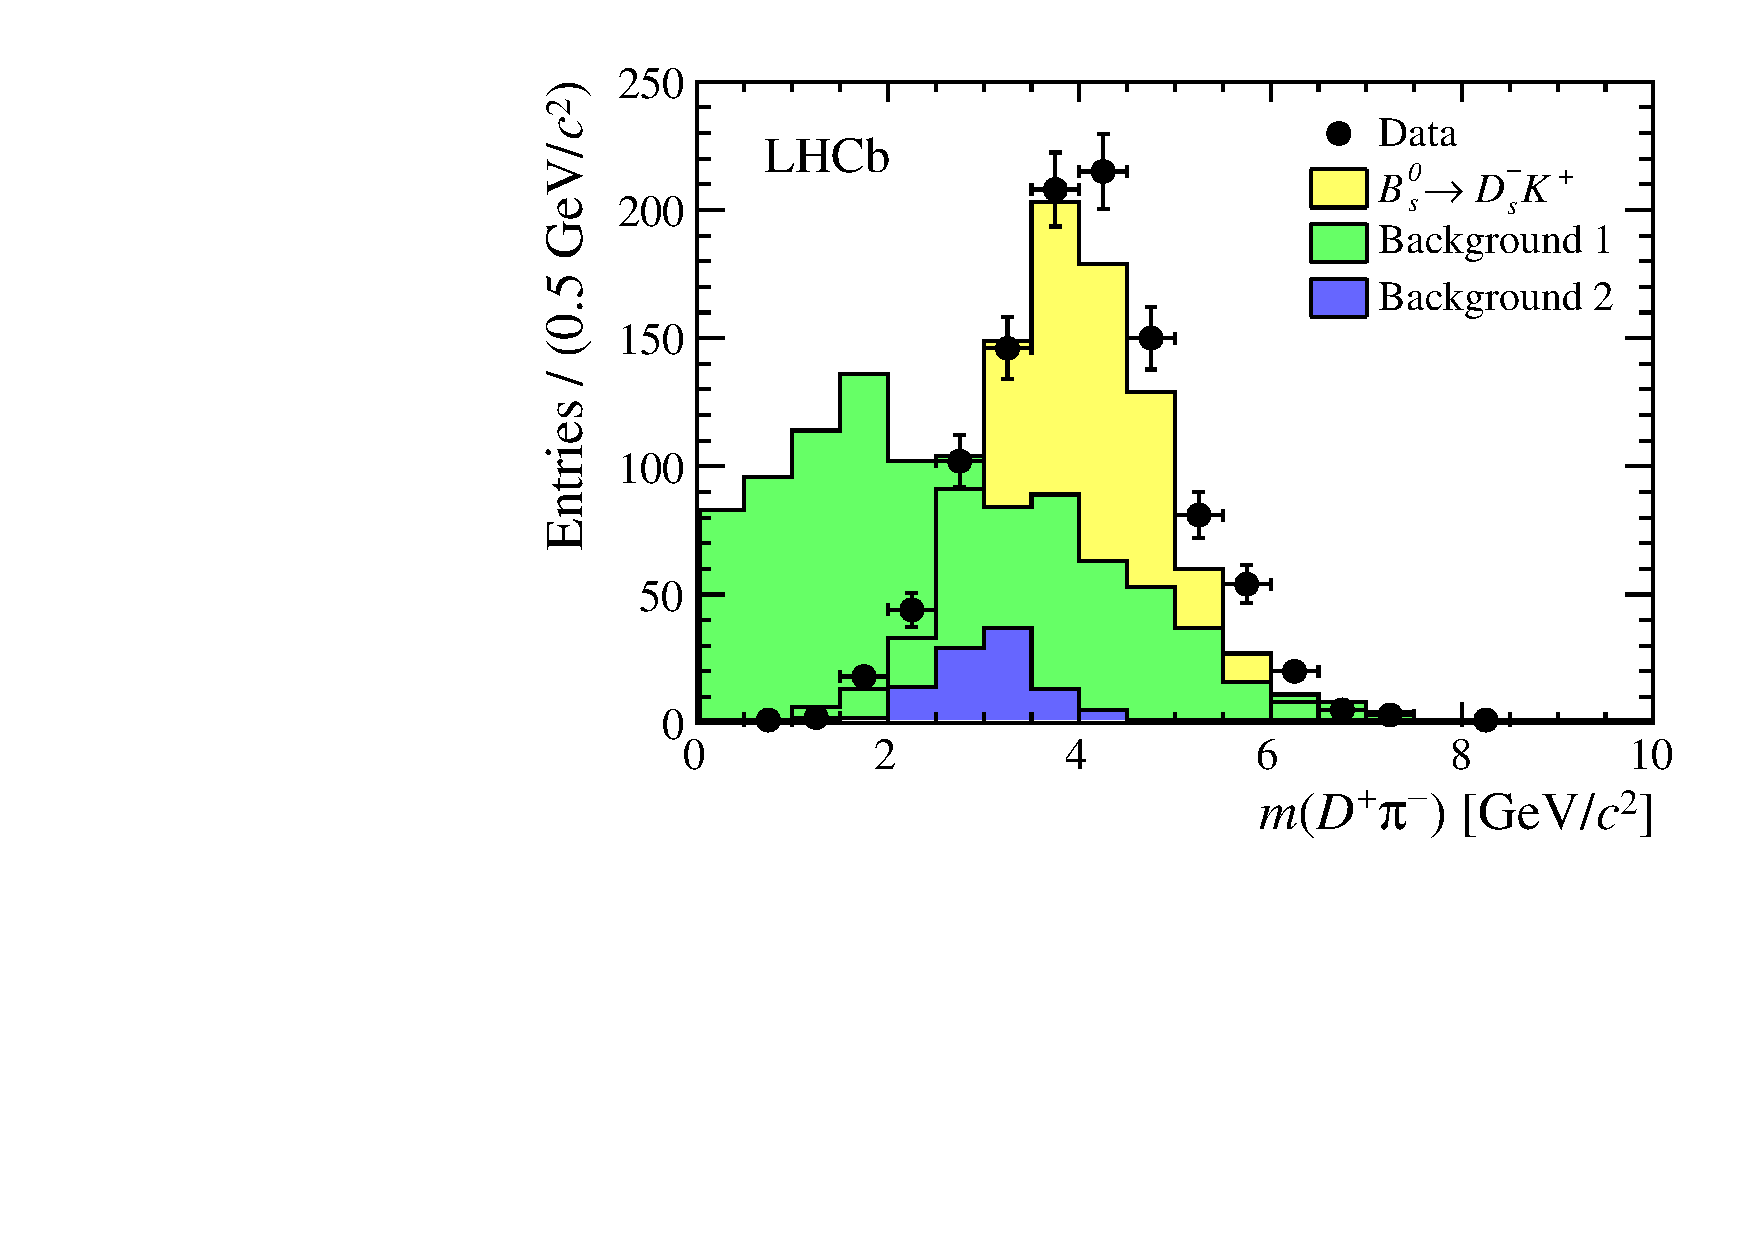
\includegraphics[width=0.49\linewidth]{Example1DPlot-python-1}\put(-32,133){(a)}
    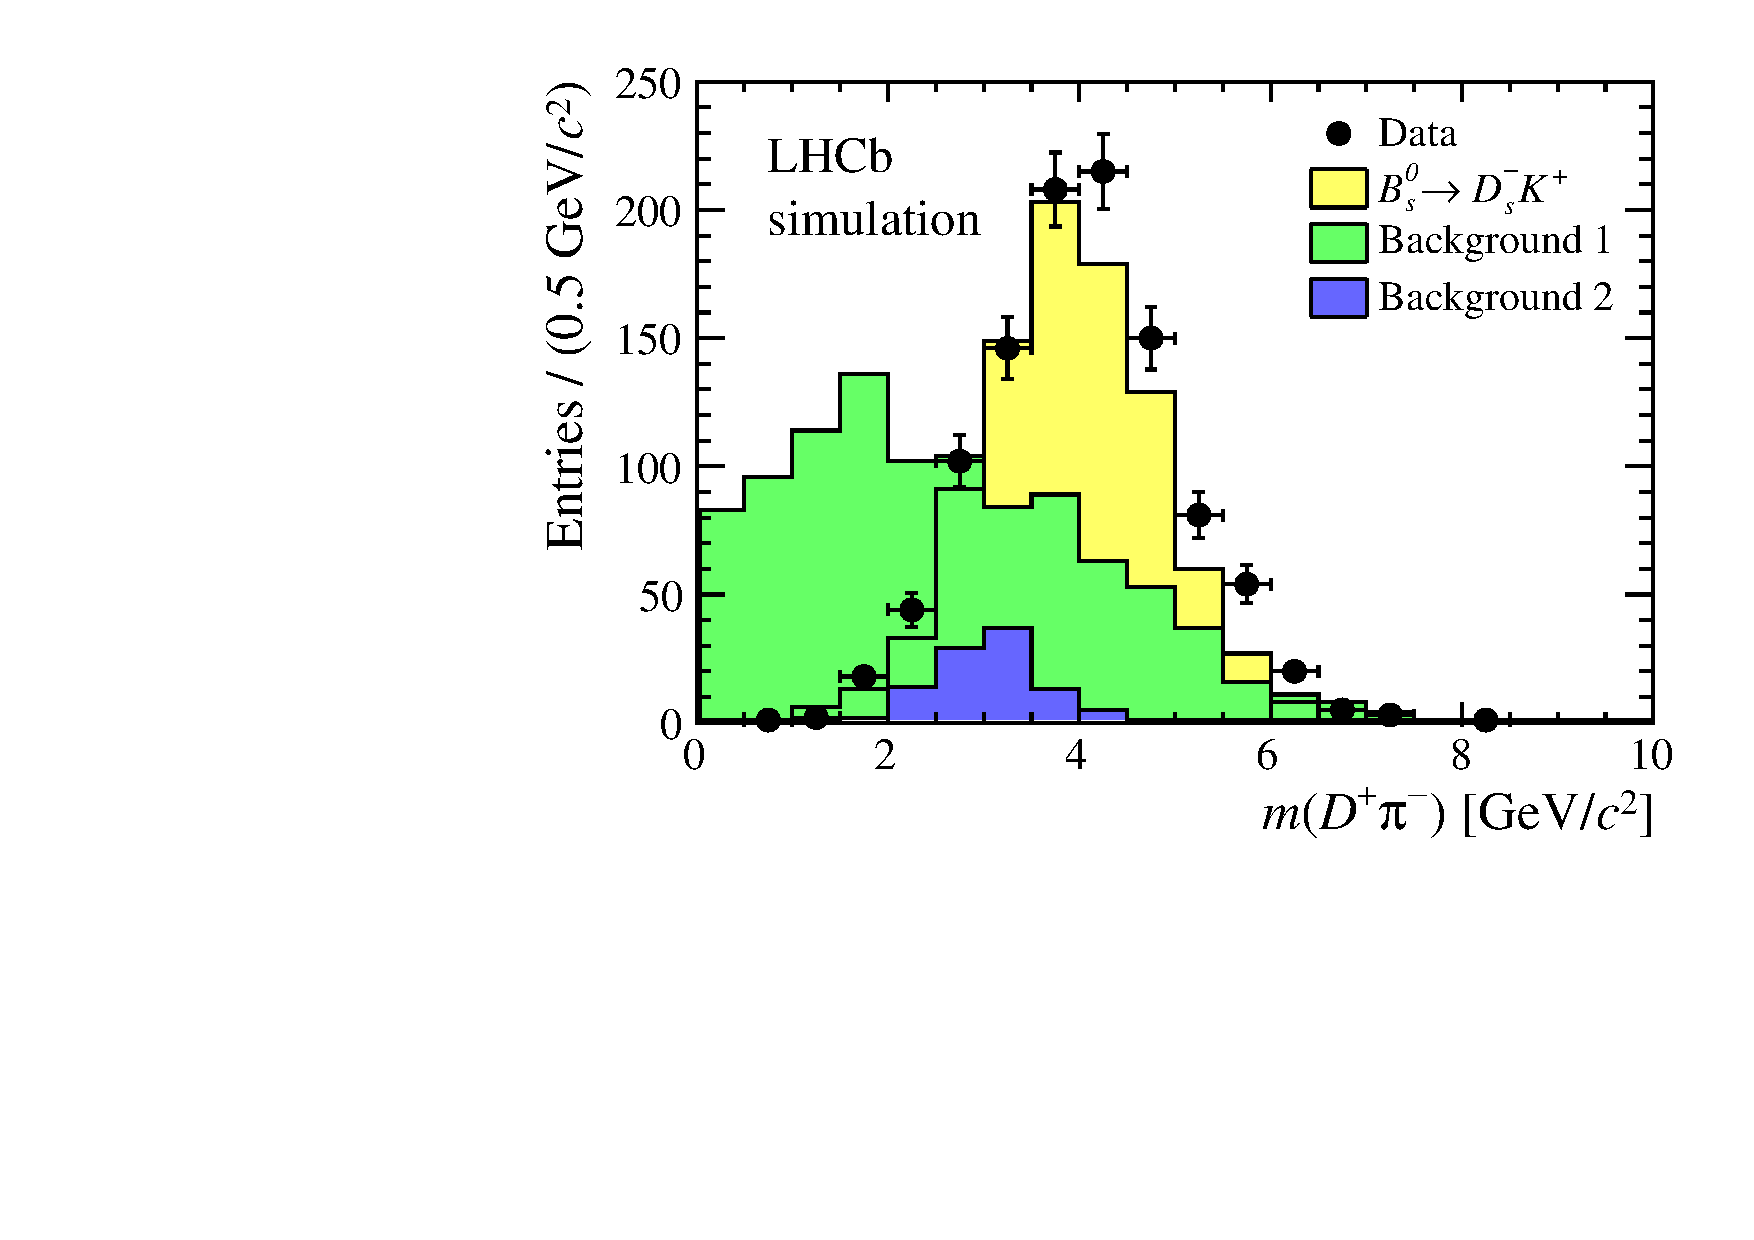
\includegraphics[width=0.49\linewidth]{Example1DPlot-python-1_sim}\put(-32,133){(b)}
    \vspace*{-0.5cm}
  \end{center}
  \caption{
    %\small %captions should be a little bit smaller than main text
    Example plots for (a) data and (b) simulation using the \lhcb style from the \urania package
    \texttt{RootTools/LHCbStyle}. The signal data is shown as points
    with the signal component as yellow (light shaded), background 1 as green
    (medium shaded) and background 2 as blue (dark shaded).}
  \label{fig:example}
\end{figure}
%%%%%%%%%%%%%%%%%%%%%%%%%%%%%%%%%%%%%%%%

\begin{enumerate}
\item Before you make a figure you should ask yourself what message
  you want to get across. You don't make a plot ``because you can''
  but because it is the best illustration of your argument. 
  
\item Figures should be legible at the size they will appear in the
  publication, with suitable line width.  Their axes should be
  labelled, and have suitable units (e.g. avoid a mass plot with
  labels in \mevcc if the region of interest covers a few \gevcc
  and all the numbers then run together).  Spurious background shading
  and boxes around text should be avoided.

\item For the $y$-axis, ``Entries'' or ``Candidates'' is appropriate in case no
background subtraction has been applied. Otherwise ``Yield'' or ``Decays''
may be more appropriate. If the unit on the $y$-axis corresponds to 
the yield per bin, indicate so, for example ``Entries / (5\mevcc)'' or ``Entries per 5\mevcc''.


\item Fit curves should not obscure the data points, and
   data points are best (re)drawn over the fit curves. In this
   case avoid in the caption the term ``overlaid'' when
   referring to a fit curve, and instead use the words  
   ``shown'' or ``drawn''.

\item Colour may be used in figures, but the distinction between
  differently coloured areas or lines should be clear also when the
  document is printed in black and white, for example through
  differently dashed lines. The \lhcb style mentioned above implements
  a colour scheme that works well but individual adjustments might be
  required.

  In particular for two-dimensional plots, never use the default ``rainbow'' palette from \root, as both extreme values will appear dark when printed in black-and-white, or viewed by colour-blind people. Printer-friendly palettes are advised. You can make your own using \href{http://colorbrewer2.org}{\tt colorbrewer2.org}.

\item Using different hatching styles helps to distinguished filled areas, 
  also in black and white prints. Hatching styles 3001-3025 should be
  avoided since they behave unpredictably under zooming and scaling. 
  Good styles for ``falling hatched'' and ``rising hatched'' are 3345 and 3354.

\item Figures with more than one part should have the parts labelled
  (a), (b) \etc, with a corresponding description in the caption;
  alternatively they should be clearly referred to by their position,
  e.g. Fig.~1\,(left). In the caption, the labels (a), (b) \etc should
  precede their description. When referencing specific sub-figures,
  use ``see Fig. 1(a)'' or ``see Figs. 2(b)-(e)''.

\item All figures containing \lhcb data should have "{\lhcb}" written on
  them.  For preliminary results, that should be replaced by ``LHCb preliminary''.
  Figures that only have simulated data should display ``LHCb simulation''.
  Figures that do not depend on LHCb-specific software (\eg only on \pythia)
  should not have any label.
%If a figure contains data with several fit components, you should 
%add  a label "{\tt data symbol} Data"
  
  \item All figures containing \lhcb data should have the corresponding luminosity written on them.
For example, if all  Run\,1\&2 data were analysed, write "$9\ \invfb$" in a new line underneath  "{\lhcb}".
Alternatively the luminosity could be  be added as  \mbox{"{\tt data symbol} Data $9\ \invfb$"}.
For cross-section or heavy-ion papers it might be more useful to give centre-of-mass energy "$\sqrt{s} = 13 \tev$" instead of luminosity.

\item Keep captions short. They should contain the information necessary to understand the figure, but no more. For instance the fit model does not need to be repeated. Describe the data first, then mention the fit components.

\item An example diagram depicting the angles in a \decay{\Bs}{\Kstarz\Kstarzb} decay is shown in
  Fig.~\ref{fig:diagram}.
  The source code is provided in \verb!figs/diagram.tex! and can be adapted to any four-body
  decay.\footnote{This is example of a footnote that goes below a floating object thanks to the {\tt footmisc}
    package. Some argue this is horrid.}
\end{enumerate}
%%%%%%%%%%%%%%%%%%%%%%%%%%%%%%%%%%%%%%%%
\begin{figure}[b] % bootom to show footmisc
  \begin{center}
    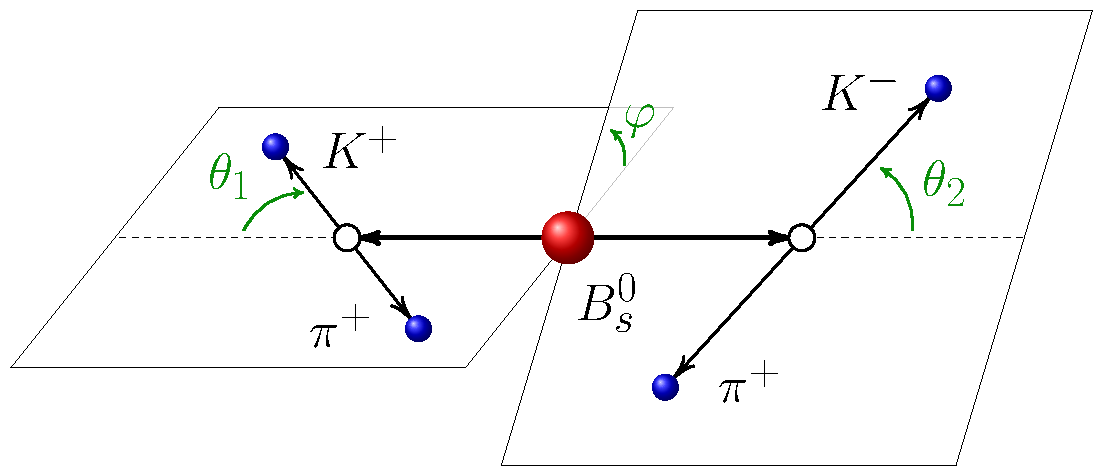
\includegraphics[width=0.7\linewidth]{diagram}
  \end{center}
  \caption{Definition of the angles $\theta_1$, $\theta_1$ and $\varphi$
   in the \decay{\Bs}{\Kstarz\Kstarzb} decay. Image by Julian Garcia Pardinas.}
  \label{fig:diagram}
\end{figure}
%%%%%%%%%%%%%%%%%%%%%%%%%%%%%%%%%%%%%%%%

%%%%%%%%%%%%%%%%%%%%%%%%%%%%%%%%%%%%%%%%%%%%%%%%%%%%%%%%%%%%%%%%%%%%%%%%%%%%%%%%%%%%%%%%%%%%%%%%%
\section{References}
\label{sec:References}

References should be made using Bib\TeX~\cite{BibTeX}. A special style
\texttt{LHCb.bst} has been created to achieve a uniform
style. Independent of the journal the paper is submitted to, the
preprint should be created using this style. Where arXiv numbers
exist, these should be added even for published articles. In the PDF
file, hyperlinks will be created to both the arXiv and the published
version, using the {\tt doi} for the latter.

Results from other experiments should be cited even if not yet published. 

\begin{enumerate}

\item Citations are marked using square brackets, and the
  corresponding references should be typeset using Bib\TeX\ and the
  official \lhcb Bib\TeX\ style. 

\item For references with four or less authors all of the authors'
  names are listed~\cite{Lee:1967iu}, otherwise the first author
  is given, followed by \etal. The \lhcb Bib\TeX\ style will
  take care of this. The limit of four names can be changed by changing the number 4 in 
  ``{\tt \#4 'max.num.names.before.forced.et.al :=}''
  in {\tt LHCb.bst}, as was done in Ref.~\cite{LHCb-PAPER-2017-038}.

\item The order of references should be sequential when reading the
  document. This is automatic when using Bib\TeX.

\item The titles of papers should in general be included. To remove
  them, change \texttt{\textbackslash
    setboolean\{articletitles\}\{false\}} to \texttt{true} at the top
  of this template.

\item Whenever possible, use references from the supplied files
\verb!main.bib!, \verb!LHCb-PAPER.bib!, \verb!LHCb-CONF.bib!, and \verb!LHCB-DP.bib!.
These are kept up-to-date by the EB. If you see a mistake, do not edit these files,
but let the EB know. This way, for every update of the paper, you save
yourself the work of updating the references. Instead, you can just copy or
check in the latest versions of the \verb!.bib! files from the repository.
{\bf Do not take these references from \texttt{inspirehep} instead} (``{\tt Aaaij:20XXxyz}''), as \texttt{inspirehep} sometimes adds mistakes, does not handle errata properly and does not use LHCb-specific macros.

\item For those references not provided by the EB, the best
  is to copy the Bib\TeX\ entry directly from
  \href{http://inspirehep.net}{inspirehep}.
    Often these need to be edited to get the 
  correct title, author names and formatting. The warning about special UTF8 characters should never be ignored. It usually signals a accentuated character in an author name.
  For authors with multiple initials, add a space between them (change \texttt{R.G.C.} to \texttt{R. G. C.}),
  otherwise only the first initial will be taken. 
  Also, make sure to eliminate unnecessary capitalisation.
  Apart from that, the title should be respected as much as possible
  (\eg do not change particle names to PDG convention nor introduce/remove factors of $c$, but do change Greek capital letters to use our slanted font.).
  Check that both the arXiv and the journal index are clickable
  and point to the right article.

%\item Even if the basic formatting of the Bib\TeX\ entry is taken from
%  \texttt{Inspire}, all the data should be cross checked against the
%  journal. Often there are minor changes to author initials or
%  titles. In case of a difference between the preprint and the
%  journal, the bibliographic information from the journal should be
%  used.

\item The \texttt{mciteplus}~\cite{mciteplus} package is used
  to enable multiple references to show up as a single item in the
  reference list. As an example \texttt{\textbackslash
    cite\{Cabibbo:1963yz,*Kobayashi:1973fv\}} where the \texttt{*}
  indicates that the reference should be merged with the previous
  one. The result of this can be seen in
  Ref.~\cite{Cabibbo:1963yz,*Kobayashi:1973fv}. Be aware that the
  \texttt{mciteplus} package should be included as the very last item
  before the \texttt{\textbackslash begin\{document\}} to work
  correctly.

\item It should be avoided to make references to public notes and
  conference reports in public documents. Exceptions can be discussed
  on a case-by-case basis with the review committee for the
  analysis. In internal reports they are of course welcome and can be
  referenced as seen in Ref.~\cite{LHCb-CONF-2012-013} using the
  \texttt{lhcbreport} category. For conference reports, omit the
  author field completely in the Bib\TeX\ record.

\item To get the typesetting and hyperlinks correct for \lhcb reports,
  the category \texttt{lhcbreport} should be used in the Bib\TeX\
  file. See Refs.~\cite{LHCb-INT-2011-047, *LHCb-ANA-2011-078,
    *CERN-THESIS-2014-057, *LHCb-PROC-2014-017, *LHCb-TALK-2014-257}
  for some examples. It can be used for \lhcb documents in the series
  \texttt{CONF}, \texttt{PAPER}, \texttt{PROC}, \texttt{THESIS},
  \texttt{LHCC}, \texttt{TDR} and internal \lhcb reports. Papers sent
  for publication, but not published yet, should be referred with
  their \texttt{arXiv} number, so the \texttt{PAPER} category should
  only be used in the rare case of a forward reference to a paper.

\item Proceedings can be used for references to items such as the
  \lhcb simulation~\cite{LHCb-PROC-2011-006}, where we do not yet have
  a published paper.

\end{enumerate}

There is a set of standard references to be used in \lhcb that are
listed in Appendix~\ref{sec:StandardReferences}.


% Do not include this in any draft (just for information in the template)
\section{Acknowledgements paragraph}

Include the following text in the Acknowledgements section in all paper
drafts. It is not needed for analysis notes or conference reports.

The text below are the acknowledgements as approved by the collaboration
board. Extending the acknowledgements to include individuals from outside the
collaboration who have contributed to the analysis should be approved by the
EB. The extra acknowledgements are normally placed before the standard 
acknowledgements, unless it matches better with the text of the standard 
acknowledgements to put them elsewhere. They should be included in the draft 
for the first circulation. Except in exceptional circumstances, to be approved by the
EB chair, authors of the paper should not be named in extended acknowledgements.

%\vspace{1cm}

\section*{Acknowledgements}
%
% These Acknowledgements valid from 3-May-2019
%
We express our gratitute to Elena Gonzalez Ferreiro for the co-mover model predictions and YanQing Ma for the NRQCD model predictions.
We express our gratitude to our colleagues in the CERN
accelerator departments for the excellent performance of the LHC. We
thank the technical and administrative staff at the LHCb
institutes.
We acknowledge support from CERN and from the national agencies:
CAPES, CNPq, FAPERJ and FINEP (Brazil); 
MOST and NSFC (China); 
CNRS/IN2P3 (France); 
BMBF, DFG and MPG (Germany); 
INFN (Italy); 
NWO (Netherlands); 
MNiSW and NCN (Poland); 
MCID/IFA (Romania); 
%MSHE (Russia); 
MICINN (Spain); 
SNSF and SER (Switzerland); 
NASU (Ukraine); 
STFC (United Kingdom); 
DOE NP and NSF (USA).
We acknowledge the computing resources that are provided by CERN, IN2P3
(France), KIT and DESY (Germany), INFN (Italy), SURF (Netherlands),
PIC (Spain), GridPP (United Kingdom), 
%RRCKI and Yandex LLC (Russia), 
CSCS (Switzerland), IFIN-HH (Romania), CBPF (Brazil),
and Polish WLCG (Poland).
We are indebted to the communities behind the multiple open-source
software packages on which we depend.
Individual groups or members have received support from
ARC and ARDC (Australia);
Key Research Program of Frontier Sciences of CAS, CAS PIFI, CAS CCEPP, 
Fundamental Research Funds for the Central Universities, 
and Sci. \& Tech. Program of Guangzhou (China);
Minciencias (Colombia);
EPLANET, Marie Sk\l{}odowska-Curie Actions, ERC and NextGenerationEU (European Union);
A*MIDEX, ANR, IPhU and Labex P2IO, and R\'{e}gion Auvergne-Rh\^{o}ne-Alpes (France);
%RFBR, RSF and Yandex LLC (Russia);
AvH Foundation (Germany);
ICSC (Italy); 
GVA, XuntaGal, GENCAT, Inditex, InTalent and Prog.~Atracci\'on Talento, CM (Spain);
SRC (Sweden);
the Leverhulme Trust, the Royal Society
 and UKRI (United Kingdom).

% Comment this in for paper drafts; do not include this in analysis note, conference and figure reports
%\section*{Acknowledgements}
%
% These Acknowledgements valid from 3-May-2019
%
We express our gratitute to Elena Gonzalez Ferreiro for the co-mover model predictions and YanQing Ma for the NRQCD model predictions.
We express our gratitude to our colleagues in the CERN
accelerator departments for the excellent performance of the LHC. We
thank the technical and administrative staff at the LHCb
institutes.
We acknowledge support from CERN and from the national agencies:
CAPES, CNPq, FAPERJ and FINEP (Brazil); 
MOST and NSFC (China); 
CNRS/IN2P3 (France); 
BMBF, DFG and MPG (Germany); 
INFN (Italy); 
NWO (Netherlands); 
MNiSW and NCN (Poland); 
MCID/IFA (Romania); 
%MSHE (Russia); 
MICINN (Spain); 
SNSF and SER (Switzerland); 
NASU (Ukraine); 
STFC (United Kingdom); 
DOE NP and NSF (USA).
We acknowledge the computing resources that are provided by CERN, IN2P3
(France), KIT and DESY (Germany), INFN (Italy), SURF (Netherlands),
PIC (Spain), GridPP (United Kingdom), 
%RRCKI and Yandex LLC (Russia), 
CSCS (Switzerland), IFIN-HH (Romania), CBPF (Brazil),
and Polish WLCG (Poland).
We are indebted to the communities behind the multiple open-source
software packages on which we depend.
Individual groups or members have received support from
ARC and ARDC (Australia);
Key Research Program of Frontier Sciences of CAS, CAS PIFI, CAS CCEPP, 
Fundamental Research Funds for the Central Universities, 
and Sci. \& Tech. Program of Guangzhou (China);
Minciencias (Colombia);
EPLANET, Marie Sk\l{}odowska-Curie Actions, ERC and NextGenerationEU (European Union);
A*MIDEX, ANR, IPhU and Labex P2IO, and R\'{e}gion Auvergne-Rh\^{o}ne-Alpes (France);
%RFBR, RSF and Yandex LLC (Russia);
AvH Foundation (Germany);
ICSC (Italy); 
GVA, XuntaGal, GENCAT, Inditex, InTalent and Prog.~Atracci\'on Talento, CM (Spain);
SRC (Sweden);
the Leverhulme Trust, the Royal Society
 and UKRI (United Kingdom).

\section{Inclusion of supplementary material}
\label{sec:Supplementary}

Three types of supplementary material should be distinguished:
\begin{itemize}
\item{A regular appendix: lengthy equations or long tables are sometimes
better put in an appendix in order not to interrupt the main flow of a paper.
Appendices will appear in the final paper, on arXiv
and on the CDS record and should be considered integral
part of a paper, and are thus to be reviewed like the rest of the paper.
An example of an LHCb paper with an appendix is Ref.~\cite{LHCb-PAPER-2013-070}.
}
\item{Supplementary material for CDS: plots or tables that 
would make the paper exceed the page limit or are
not appropriate to include in the paper itself,
but are desirable to be shown in public
should be added to the paper drafts in an appendix, and
removed from the paper before submitting to arXiv or the journal.
See Appendix~\ref{sec:Supplementary-App} for further instructions.
Examples are: comparison plots of the new result with older results,
plots that illustrate cross-checks.
An example of an LHCb paper with supplementary material for CDS 
is Ref.~\cite{LHCb-PAPER-2013-035}.
Supplementary material for CDS cannot be referenced in the paper.
Supplementary material should be included in the draft paper to be
reviewed by the collaboration.
}
\item{Supplementary material for the paper. This is usually called ``supplemental material'', which distinguishes it from supplementary material for CDS only. Most journals allow
to submit files along with the paper that will not be part of the
text of the article, but will be stored on the journal server.
Examples are plain text files with numerical data corresponding to the plots
in the paper. 
The supplemental material should be cited in the paper by including a reference
which should say ``See supplemental material at [link] for [give brief description of material].''
The journal will insert a specific link for [link]. The arXiv version will usually include the supplemental material as part of the paper and so should not contain the words ``at [link]''.
Supplemental material should be included in the draft paper to be
reviewed by the collaboration.
An example of an LHCb paper with supplemental material 
is Ref.~\cite{LHCb-PAPER-2015-029}
}
\end{itemize}



% ===============================================================================
% Purpose: appendix to the standard template: standard symbol alises from Ulrik
% Author: Tomasz Skwarnicki
% Created on: 2009-09-24
% ===============================================================================

%{\noindent\normalfont\bfseries\Large Appendices}
\section*{Appendices}

\appendix

\section{Standard References}
\label{sec:StandardReferences}
Below is a list of common references, as
well as a list of all \lhcb publications.
As they are already in prepared bib files, they can be used as simply as
\texttt{\textbackslash cite\{LHCb-DP-2008-001\}} to get the \lhcb detector paper.
The references are defined in the files \texttt{main.bib},  \texttt{LHCb-PAPER.bib},
\texttt{LHCb-CONF.bib}, \texttt{LHCb-DP.bib} \texttt{LHCb-TDR.bib} files, with obvious contents.
Each of these have their \texttt{LHCb-ZZZ-20XX-0YY} number as their cite code.
If you believe there is a problem with the formatting or
content of one of the entries, then get in contact with the Editorial
Board rather than just editing it in your local file,
since you are likely to need the latest version just before submitting the article.

%%%%%%%%%%%%%%%%%%%%%%%%%%%%%%%%%%
\newcommand{\showcite}[1]{\texttt{#1}~\cite{#1}}%
\newcommand{\revshowcite}[1]{\begin{minipage}{1cm}\cite{#1}\end{minipage}\texttt{#1}}%
%%%%%%%%%%%%%%%%%%%%%%%%%%%%%%%%%%
\begin{center}
  \begin{longtable}{ll}
\caption{\small Standard references.}\label{tab:Refs}
\endfirsthead
\multicolumn{2}{c}{ -- continued from previous page.}
\endhead
\endfoot
\endlastfoot
\hline
Description & \begin{minipage}{1cm}Ref.\end{minipage}\texttt{cite} code \\
\hline % standard physics papers
Lee, Weinberg, Zumino & \revshowcite{Lee:1967iu}  \\ % {Weinberg:1967} \\
Cabibbo, Kobayashi, Maskawa & \revshowcite{Cabibbo:1963yz,*Kobayashi:1973fv}  \\ % {Cabibbo:1963yz,*Kobayashi:1973fv} \\
Gell-Mann, Zweig & \revshowcite{GellMann:1964nj,*Zweig:352337}  \\ % {GellMann:1964nj,*Zweig:352337} \\
Baryon asymmetry \& SM \CP &  \revshowcite{Gavela:1994dt}  \\ % {Gavela:1994dt} \\
Baryon asymmetry \& SM \CP &  \revshowcite{Gavela:1993ts}  \\ % {Gavela:1993ts} \\
EW Baryogenesis \& \CP &  \revshowcite{Huet:1994jb}  \\ % {Huet:1994jb} \\
Dalitz Plot\footnote{Dalitz invented the method, Fabri added relativistic corrections.} & \revshowcite{Dalitz:1953cp,*Fabri:1954zz} \\
\hline % physics resources
PDG 2020  & \revshowcite{PDG2020} \\
PDG 2019  & \revshowcite{PDG2019} \\
PDG 2018 & \revshowcite{PDG2018} \\
PDG 2016 & \revshowcite{PDG2016}  \\ % {PDG2016} \\
PDG 2014 & \revshowcite{PDG2014}  \\ % {PDG2014} \\
HFlav 2018 & \revshowcite{HFLAV18}  \\ 
HFlav 2016 & \revshowcite{HFLAV16}  \\ 
HFlav (pre-2016)  & \revshowcite{Amhis:2014hma}  \\ 
CKMfitter group & \revshowcite{CKMfitter2005}  \\ % {CKMfitter2005} \\
CKMfitter group & \revshowcite{CKMfitter2015}  \\ % {CKMfitter2015} \\
UTfit (Standard Model/CKM) & \revshowcite{UTfit-UT}  \\ % {UTfit-UT} \\
UTfit (New Physics) & \revshowcite{UTfit-NP}  \\ % {UTfit-NP} \\
\hline % computing
\pythia & \revshowcite{Sjostrand:2007gs,*Sjostrand:2006za}  \\ 
\lhcb \pythia tuning & \revshowcite{LHCb-PROC-2010-056}  \\ % {LHCb-PROC-2010-056} \\
\evtgen & \revshowcite{Lange:2001uf}   \\ % {Lange:2001uf} \\
%\photos & \revshowcite{Golonka:2005pn}   \\ % {Golonka:2005pn} \\
\photos & \revshowcite{davidson2015photos}   \\ % {davidson2015photos} \\
\geant & \revshowcite{Allison:2006ve, *Agostinelli:2002hh}  \\ % {Allison:2006ve, *Agostinelli:2002hh} \\
\lhcb simulation & \revshowcite{LHCb-PROC-2011-006}  \\ % {LHCb-PROC-2011-006} \\
RapidSim & \revshowcite{Cowan:2016tnm}  \\ % {Cowan:2016tnm} \\
\dirac & \revshowcite{Tsaregorodtsev:2010zz,*BelleDIRAC}  \\ % {Tsaregorodtsev:2010zz, *BelleDIRAC}  \\
\hline % LHCb-specific
HLT2 topological trigger & \revshowcite{BBDT}  \\ % {BBDT} \\
Topological trigger reoptimization --- Run 2 & \revshowcite{LHCb-PROC-2015-018}\\
Turbo and real-time alignment --- Run 2 & \revshowcite{LHCb-PROC-2015-011}  \\
TisTos method & \revshowcite{LHCb-PUB-2014-039}  \\
Allen &  \revshowcite{Aaij:2019zbu}  \\
PIDCalib (for Run~1) & \revshowcite{LHCb-PUB-2016-021}  \\ % {LHCb-PUB-2016-021} \\
Ghost probability & \revshowcite{DeCian:2255039}  \\ % {DeCian:2255039}\\
Primary vertex reconstruction & \revshowcite{Kucharczyk:1756296} \\
DecayTreeFitter & \revshowcite{Hulsbergen:2005pu}  \\ % {Hulsbergen:2005pu} \\
SMOG & \revshowcite{FerroLuzzi:2005em}  \\ % {FerroLuzzi:2005em} \\
Run-2 tagging & \revshowcite{Fazzini:2018dyq}\\
OS \kaon, \muon, \electron and VS tagging & \revshowcite{LHCb-PAPER-2011-027}\\
OS charm tagging & \revshowcite{LHCb-PAPER-2015-027}\\
SS kaon tagging & \revshowcite{LHCb-PAPER-2015-056}\\
SS proton and pion tagging & \revshowcite{LHCb-PAPER-2016-039}\\
Reommendations for multiple candidates & \revshowcite{Koppenburg:2017zsh} \\
\multicolumn{2}{l}{See also Table~\ref{tab:LHCb-DPs} for LHCb performance references.}\\
\hline % selection
\sPlot & \revshowcite{Pivk:2004ty}  \\ % {Pivk:2004ty} \\
sFit & \revshowcite{Xie:2009rka}  \\ % {Xie:2009rka} \\
Punzi's optimization & \revshowcite{Punzi:2003bu}  \\ % {Punzi:2003bu} \\
BDT & \revshowcite{Breiman}  \\ % {Breiman} \\
BDT training & \revshowcite{AdaBoost}  \\ % {AdaBoost} \\
TMVA\footnote{Do not cite this instead of the actual reference for the MVA being used.}  & \revshowcite{Hocker:2007ht,*TMVA4}  \\ % {Hocker:2007ht,*TMVA4} \\
RooUnfold & \revshowcite{Adye:2011gm}  \\ % {Adye:2011gm} \\
scikit-learn & \revshowcite{Scikit-learn-paper}  \\ % {Scikit-learn-paper} \\
\textsc{Laura}$^{++}$ & \revshowcite{Back:2017zqt}  \\ % {Back:2017zqt} \\
\texttt{hep\_ml} & \revshowcite{Rogozhnikov:2016bdp}  \\ % {Rogozhnikov:2016bdp} \\
\texttt{root\_numpy} & \revshowcite{root-numpy}  \\
\texttt{GammaCombo}\footnote{Always cite this along with Ref.~\cite{LHCb-PAPER-2016-032} as {\tt\textbackslash{}cite\{GammaCombo,*LHCb-PAPER-2016-032\}} (unless {\tt LHCb-PAPER-2016-032} is cited elsewhere).} & \revshowcite{GammaCombo}  \\
\tensorflow & \revshowcite{tensorflow2015-whitepaper}  \\ % {tensorflow2015-whitepaper} \\
\hline % Fits
Crystal Ball function\footnote{A valid alternative for most papers where the normalisation is not critical is to use the expression``Gaussian function with a low-mass power-law tail'' or ``Gaussian function with power-law tails''. In that case, no citation is needed} & \revshowcite{Skwarnicki:1986xj}  \\ % {Skwarnicki:1986xj} \\
Hypatia function & \revshowcite{Santos:2013gra}  \\ % {Santos:2013gra}\\
Modified Novosibirsk function & \revshowcite{Ikeda:1999aq} \\
Bukin function & \revshowcite{Bukin:2007} \\
Wilks' theorem & \revshowcite{Wilks:1938dza}  \\ % {Wilks:1938dza}\\
CL$_s$ method & \revshowcite{CLs}  \\ % {CLs} \\
BLUE method & \revshowcite{Nisius:2020jmf}  \\ 
Bootstrapping & \revshowcite{efron:1979}  \\ % {efron:1979} \\
Blatt--Weisskopf barrier & \revshowcite{Blatt:1952ije}  \\ % {Blatt:1952ije} \\
\hline % LHC
$f_s/f_d$ at 7--8\tev & \revshowcite{fsfd}  \\ % {fsfd} \\
LHC beam energy uncertainty  & \revshowcite{PhysRevAccelBeams.20.081003}  \\ % {PhysRevAccelBeams.20.081003}\\
\hline
\end{longtable}
%  \end{tabular}
\end{center}

\begin{center}
\begin{longtable}{ll}
\caption{\small LHCb detector performance papers.}\label{tab:LHCb-DPs}
\endfirsthead
\multicolumn{2}{c}{ -- continued from previous page.}
\endhead
\endfoot
\endlastfoot
\hline
    \hline
    \texttt{LHCb-DP} number & Title \\
    \hline
    \showcite{LHCb-DP-2021-005} &  {\small TBD}\\
    \showcite{LHCb-DP-2021-004} &  {\small TBD}\\
    \showcite{LHCb-DP-2021-003} &  {\small TBD}\\
    \showcite{LHCb-DP-2021-002} &  {\small Centrality determination in heavy-ion collisions with the LHCb detector}\\
    \showcite{LHCb-DP-2021-001} &  {\small TBD}\\
    \showcite{LHCb-DP-2020-003} &  {\small TBD}\\
    \showcite{LHCb-DP-2020-002} &  {\small TBD}\\
    \showcite{LHCb-DP-2020-001} &  {\small TBD}\\
    \showcite{LHCb-DP-2019-006} &  {\small TBD}\\
    \showcite{LHCb-DP-2019-005} &  {\small TBD}\\
    \showcite{LHCb-DP-2019-004} &  {\small Diphoton discrimination}\\
    \showcite{LHCb-DP-2019-003} &  {\small Electron reconstruction efficiency}\\
    \showcite{LHCb-DP-2019-002} &  {\small Real-Time analysis}\\
    \showcite{LHCb-DP-2019-001} &  {\small Run~2 trigger performance}\\
    \showcite{LHCb-DP-2018-004} &  {\small ReDecay}\\
    \showcite{LHCb-DP-2018-003} &  {\small Radiation damage in TT}\\
    \showcite{LHCb-DP-2018-002} &  {\small VeLo material map using SMOG}\\
    \showcite{LHCb-DP-2018-001} &  {\small PIDCalib for Run 2 (use Ref.~\cite{LHCb-PUB-2016-021} for Run~1)} \\
    \showcite{LHCb-DP-2017-001} &  {\small Performance of the Outer Tracker --- Run 2}\\
    \showcite{LHCb-DP-2016-003} &  {\small HeRSCheL} \\
    \showcite{LHCb-DP-2016-001} &  {\small TESLA project --- Run 2} \\
    \showcite{LHCb-DP-2014-002} &  {\small LHCb detector performance} \\
    \showcite{LHCb-DP-2014-001} &  {\small Performance of the LHCb Vertex Locator} \\
%    \showcite{LHCb-DP-2013-004} &  {\small Performance of the LHCb calorimeters} \\
    \showcite{LHCb-DP-2013-003} &  {\small Performance of the LHCb Outer Tracker --- Run 1} \\
    \showcite{LHCb-DP-2013-002} &  {\small Measurement of the track reconstruction efficiency at LHCb} \\
    \showcite{LHCb-DP-2013-001} &  {\small Performance of the muon identification at LHCb} \\
    \showcite{LHCb-DP-2012-005} &  {\small Radiation damage in the LHCb Vertex Locator} \\
    \showcite{LHCb-DP-2012-004} &  {\small The \lhcb trigger and its performance in 2011} \\
    \showcite{LHCb-DP-2012-003} &  {\small Performance of the \lhcb RICH detector at the LHC} \\
    \showcite{LHCb-DP-2012-002} &  {\small Performance of the LHCb muon system} \\
    \showcite{LHCb-DP-2012-001} &  {\small Radiation hardness of the LHCb Outer Tracker} \\
    \showcite{LHCb-DP-2011-002} &  {\small Simulation of machine induced background \dots} \\
    \showcite{LHCb-DP-2011-001} &  {\small Performance of the LHCb muon system with cosmic rays} \\
    \showcite{LHCb-DP-2010-001} &  {\small First spatial alignment of the LHCb VELO \dots} \\
    \showcite{LHCb-DP-2008-001} &  {\small \lhcb detector} \\
    \hline
  \end{longtable}
\end{center}

\begin{center}
\begin{longtable}{ll}
\caption{\small LHCb TDRs.}\label{tab:LHCb-TDRs}
\endfirsthead
\multicolumn{2}{c}{ -- continued from previous page.}
\endhead
\endfoot
\endlastfoot
    \hline
    \texttt{LHCb-TDR} number & Title \\
    \hline
    \showcite{LHCb-TDR-023} & {\small Framework TDR for LHCb Upgrade II} \\
    \showcite{LHCb-TDR-022} & {\small PLUME} \\
    \showcite{LHCb-TDR-021} & {\small Allen} \\
    \showcite{LHCb-TDR-020} & {\small SMOG Upgrade} \\
    \showcite{LHCb-TDR-018} & {\small Upgrade computing model} \\
    \showcite{LHCb-PII-Physics} & {\small Phase-II upgrade physics case} \\
    \showcite{LHCb-PII-EoI} & {\small Expression of interest for Phase-II upgrade} \\
    \showcite{LHCb-TDR-017} & {\small Upgrade software and computing} \\
    \showcite{LHCb-TDR-016} & {\small Trigger and online upgrade} \\
    \showcite{LHCb-TDR-015} & {\small Tracker upgrade} \\
    \showcite{LHCb-TDR-014} & {\small PID upgrade} \\
    \showcite{LHCb-TDR-013} & {\small VELO upgrade} \\
    \showcite{LHCb-TDR-012} & {\small Framework TDR for the upgrade} \\
    \showcite{LHCb-TDR-011} & {\small Computing} \\
    \showcite{LHCb-TDR-010} & {\small Trigger} \\
    \showcite{LHCb-TDR-009} & {\small Reoptimized detector} \\
    \showcite{LHCb-TDR-008} & {\small Inner Tracker} \\
    \showcite{LHCb-TDR-007} & {\small Online, DAQ, ECS} \\
    \showcite{LHCb-TDR-006} & {\small Outer Tracker} \\
    \showcite{LHCb-TDR-005} & {\small VELO} \\
    \showcite{LHCb-TDR-004} & {\small Muon system} \\
    \showcite{LHCb-TDR-003} & {\small RICH} \\
    \showcite{LHCb-TDR-002} & {\small Calorimeters} \\
    \showcite{LHCb-TDR-001} & {\small Magnet} \\
    \hline
  \end{longtable}
\end{center}

{\tiny\begin{center}
%  \begin{tabular}{l|l}
\begin{longtable}{lllll}
\caption{\small
  LHCb-PAPERs (which have their identifier as their cite code).
  DNE: Does not exist.
}
\label{tab:LHCb-PAPERs}
\endfirsthead
\multicolumn{5}{c}{ -- continued from previous page.}
\endhead
\endfoot
\endlastfoot
\showcite{LHCb-PAPER-2022-020}  &
\showcite{LHCb-PAPER-2022-019}  &
\showcite{LHCb-PAPER-2022-018}  &
\showcite{LHCb-PAPER-2022-017}  &
\showcite{LHCb-PAPER-2022-016} \\
\showcite{LHCb-PAPER-2022-015}  &
\showcite{LHCb-PAPER-2022-014}  &
\showcite{LHCb-PAPER-2022-013}  &
\showcite{LHCb-PAPER-2022-012}  &
\showcite{LHCb-PAPER-2022-011}  \\
\showcite{LHCb-PAPER-2022-010}  &
\showcite{LHCb-PAPER-2022-009}  &
\showcite{LHCb-PAPER-2022-008}  &
\showcite{LHCb-PAPER-2022-007}  &
\showcite{LHCb-PAPER-2022-006} \\
\showcite{LHCb-PAPER-2022-005}  &
\showcite{LHCb-PAPER-2022-004}  &
\showcite{LHCb-PAPER-2022-003}  &
\showcite{LHCb-PAPER-2022-002}  &
\showcite{LHCb-PAPER-2022-001}  \\
\showcite{LHCb-PAPER-2021-053}  &
\showcite{LHCb-PAPER-2021-052}  &
\showcite{LHCb-PAPER-2021-051} \\
\showcite{LHCb-PAPER-2021-050}  &
\showcite{LHCb-PAPER-2021-049}  &
\showcite{LHCb-PAPER-2021-048}  &
\showcite{LHCb-PAPER-2021-047}  &
\showcite{LHCb-PAPER-2021-046} \\
\showcite{LHCb-PAPER-2021-045}  &
\showcite{LHCb-PAPER-2021-044}  &
\showcite{LHCb-PAPER-2021-043}  &
\showcite{LHCb-PAPER-2021-042}  &
\showcite{LHCb-PAPER-2021-041} \\
\showcite{LHCb-PAPER-2021-040}  &
\showcite{LHCb-PAPER-2021-039}  &
\showcite{LHCb-PAPER-2021-038}  &
\showcite{LHCb-PAPER-2021-037}  &
\showcite{LHCb-PAPER-2021-036} \\
\showcite{LHCb-PAPER-2021-035}  &
\showcite{LHCb-PAPER-2021-034}  &
\showcite{LHCb-PAPER-2021-033}  &
\showcite{LHCb-PAPER-2021-032}  &
\showcite{LHCb-PAPER-2021-031} \\
\showcite{LHCb-PAPER-2021-030}  &
\showcite{LHCb-PAPER-2021-029}  &
\showcite{LHCb-PAPER-2021-028}  &
\showcite{LHCb-PAPER-2021-027}  &
\showcite{LHCb-PAPER-2021-026} \\
\showcite{LHCb-PAPER-2021-025}  &
\showcite{LHCb-PAPER-2021-024}  &
\showcite{LHCb-PAPER-2021-023}  &
\showcite{LHCb-PAPER-2021-022}  &
\showcite{LHCb-PAPER-2021-021} \\
\showcite{LHCb-PAPER-2021-020}  &
\showcite{LHCb-PAPER-2021-019}  &
\showcite{LHCb-PAPER-2021-018}  &
\showcite{LHCb-PAPER-2021-017}  &
\showcite{LHCb-PAPER-2021-016} \\
\showcite{LHCb-PAPER-2021-015}  &
\showcite{LHCb-PAPER-2021-014}  &
\showcite{LHCb-PAPER-2021-013}  &
\showcite{LHCb-PAPER-2021-012}  &
\showcite{LHCb-PAPER-2021-011} \\
\showcite{LHCb-PAPER-2021-010}  &
\showcite{LHCb-PAPER-2021-009}  &
\showcite{LHCb-PAPER-2021-008}  &
\showcite{LHCb-PAPER-2021-007}  &
\showcite{LHCb-PAPER-2021-006} \\
\showcite{LHCb-PAPER-2021-005}  &
\showcite{LHCb-PAPER-2021-004}  &
\showcite{LHCb-PAPER-2021-003}  &
\showcite{LHCb-PAPER-2021-002}  &
\showcite{LHCb-PAPER-2021-001} \\
\showcite{LHCb-PAPER-2020-048}  &
\showcite{LHCb-PAPER-2020-047}  &
\showcite{LHCb-PAPER-2020-046}  \\
\showcite{LHCb-PAPER-2020-045}  &
\showcite{LHCb-PAPER-2020-044}  &
\showcite{LHCb-PAPER-2020-043}  &
\showcite{LHCb-PAPER-2020-042}  &
\showcite{LHCb-PAPER-2020-041} \\
\showcite{LHCb-PAPER-2020-040}  &
\showcite{LHCb-PAPER-2020-039}  &
\showcite{LHCb-PAPER-2020-038}  &
\showcite{LHCb-PAPER-2020-037}  &
\showcite{LHCb-PAPER-2020-036} \\
\showcite{LHCb-PAPER-2020-035}  &
\showcite{LHCb-PAPER-2020-034}  &
\showcite{LHCb-PAPER-2020-033}  &
\showcite{LHCb-PAPER-2020-032}  &
\showcite{LHCb-PAPER-2020-031} \\
\showcite{LHCb-PAPER-2020-030}  &
\showcite{LHCb-PAPER-2020-029}  &
\showcite{LHCb-PAPER-2020-028}  &
\showcite{LHCb-PAPER-2020-027}  &
\showcite{LHCb-PAPER-2020-026} \\
\showcite{LHCb-PAPER-2020-025}  &
\showcite{LHCb-PAPER-2020-024}  &
\showcite{LHCb-PAPER-2020-023}  &
\showcite{LHCb-PAPER-2020-022}  &
\showcite{LHCb-PAPER-2020-021} \\
\showcite{LHCb-PAPER-2020-020}  &
\showcite{LHCb-PAPER-2020-019}  &
\showcite{LHCb-PAPER-2020-018}  &
\showcite{LHCb-PAPER-2020-017}  &
\showcite{LHCb-PAPER-2020-016} \\
\showcite{LHCb-PAPER-2020-015}  &
\showcite{LHCb-PAPER-2020-014}  &
\showcite{LHCb-PAPER-2020-013}  &
\showcite{LHCb-PAPER-2020-012}  &
\showcite{LHCb-PAPER-2020-011} \\
\showcite{LHCb-PAPER-2020-010}  &
\showcite{LHCb-PAPER-2020-009}  &
\showcite{LHCb-PAPER-2020-008}  &
\showcite{LHCb-PAPER-2020-007}  &
\showcite{LHCb-PAPER-2020-006} \\
\showcite{LHCb-PAPER-2020-005}  &
\showcite{LHCb-PAPER-2020-004}  &
\showcite{LHCb-PAPER-2020-003}  &
\showcite{LHCb-PAPER-2020-002}  &
\showcite{LHCb-PAPER-2020-001} \\
\hline
\showcite{LHCb-PAPER-2019-046} \\
\showcite{LHCb-PAPER-2019-045}  &
\showcite{LHCb-PAPER-2019-044}  &
\showcite{LHCb-PAPER-2019-043}  &
\showcite{LHCb-PAPER-2019-042}  &
\showcite{LHCb-PAPER-2019-041} \\
\showcite{LHCb-PAPER-2019-040}  &
\showcite{LHCb-PAPER-2019-039}  &
\showcite{LHCb-PAPER-2019-038}  &
\showcite{LHCb-PAPER-2019-037}  &
\showcite{LHCb-PAPER-2019-036} \\
\showcite{LHCb-PAPER-2019-035}  &
\showcite{LHCb-PAPER-2019-034}  &
\showcite{LHCb-PAPER-2019-033}  &
\showcite{LHCb-PAPER-2019-032}  &
\showcite{LHCb-PAPER-2019-031} \\
\showcite{LHCb-PAPER-2019-030}  &
\showcite{LHCb-PAPER-2019-029}  &
\showcite{LHCb-PAPER-2019-028}  &
\showcite{LHCb-PAPER-2019-027}  &
\showcite{LHCb-PAPER-2019-026} \\
\showcite{LHCb-PAPER-2019-025}  &
\showcite{LHCb-PAPER-2019-024}  &
\showcite{LHCb-PAPER-2019-023}  &
\showcite{LHCb-PAPER-2019-022}  &
\showcite{LHCb-PAPER-2019-021} \\
\showcite{LHCb-PAPER-2019-020}  &
\showcite{LHCb-PAPER-2019-019}  &
\showcite{LHCb-PAPER-2019-018}  &
\showcite{LHCb-PAPER-2019-017}  &
\showcite{LHCb-PAPER-2019-016} \\
\showcite{LHCb-PAPER-2019-015}  &
\showcite{LHCb-PAPER-2019-014}  &
\showcite{LHCb-PAPER-2019-013}  &
\showcite{LHCb-PAPER-2019-012}  &
\showcite{LHCb-PAPER-2019-011} \\
\showcite{LHCb-PAPER-2019-010}  &
\showcite{LHCb-PAPER-2019-009}  &
\showcite{LHCb-PAPER-2019-008}  &
\showcite{LHCb-PAPER-2019-007}  &
\showcite{LHCb-PAPER-2019-006} \\
\showcite{LHCb-PAPER-2019-005}  &
\showcite{LHCb-PAPER-2019-004}  &
\showcite{LHCb-PAPER-2019-003}  &
\showcite{LHCb-PAPER-2019-002}  &
\showcite{LHCb-PAPER-2019-001} \\
\hline
\showcite{LHCb-PAPER-2018-051} \\
\showcite{LHCb-PAPER-2018-050}  &
\showcite{LHCb-PAPER-2018-049}  &
\showcite{LHCb-PAPER-2018-048}  &
\showcite{LHCb-PAPER-2018-047}  &
\showcite{LHCb-PAPER-2018-046} \\
\showcite{LHCb-PAPER-2018-045}  &
\showcite{LHCb-PAPER-2018-044}  &
\showcite{LHCb-PAPER-2018-043}  &
\showcite{LHCb-PAPER-2018-042}  &
\showcite{LHCb-PAPER-2018-041} \\
\showcite{LHCb-PAPER-2018-040}  &
\showcite{LHCb-PAPER-2018-039}  &
\showcite{LHCb-PAPER-2018-038}  &
\showcite{LHCb-PAPER-2018-037}  &
\showcite{LHCb-PAPER-2018-036} \\
\showcite{LHCb-PAPER-2018-035}  &
\showcite{LHCb-PAPER-2018-034}  &
\showcite{LHCb-PAPER-2018-033}  &
\showcite{LHCb-PAPER-2018-032}  &
\showcite{LHCb-PAPER-2018-031} \\
\showcite{LHCb-PAPER-2018-030}  &
\showcite{LHCb-PAPER-2018-029}  &
\showcite{LHCb-PAPER-2018-028}  &
\showcite{LHCb-PAPER-2018-027}  &
\showcite{LHCb-PAPER-2018-026} \\
\showcite{LHCb-PAPER-2018-025}  &
\showcite{LHCb-PAPER-2018-024}  &
\showcite{LHCb-PAPER-2018-023}  &
\showcite{LHCb-PAPER-2018-022}  &
\showcite{LHCb-PAPER-2018-021} \\
\showcite{LHCb-PAPER-2018-020}  &
\showcite{LHCb-PAPER-2018-019}  &
\showcite{LHCb-PAPER-2018-018}  &
\showcite{LHCb-PAPER-2018-017}  &
\showcite{LHCb-PAPER-2018-016} \\
\showcite{LHCb-PAPER-2018-015}  &
\showcite{LHCb-PAPER-2018-014}  &
\showcite{LHCb-PAPER-2018-013}  &
\showcite{LHCb-PAPER-2018-012}  &
\showcite{LHCb-PAPER-2018-011} \\
\showcite{LHCb-PAPER-2018-010}  &
\showcite{LHCb-PAPER-2018-009}  &
\showcite{LHCb-PAPER-2018-008}  &
\showcite{LHCb-PAPER-2018-007}  &
\showcite{LHCb-PAPER-2018-006} \\
\showcite{LHCb-PAPER-2018-005}  &
\showcite{LHCb-PAPER-2018-004}  &
\showcite{LHCb-PAPER-2018-003}  &
\showcite{LHCb-PAPER-2018-002}  &
\showcite{LHCb-PAPER-2018-001} \\
\hline 
\showcite{LHCb-PAPER-2017-050}  &
\showcite{LHCb-PAPER-2017-049}  &
\showcite{LHCb-PAPER-2017-048}  &
\showcite{LHCb-PAPER-2017-047}  &
\showcite{LHCb-PAPER-2017-046} \\
\showcite{LHCb-PAPER-2017-045}  &
\showcite{LHCb-PAPER-2017-044}  &
\showcite{LHCb-PAPER-2017-043}  &
\showcite{LHCb-PAPER-2017-042}  &
\showcite{LHCb-PAPER-2017-041} \\
\showcite{LHCb-PAPER-2017-040}  &
\showcite{LHCb-PAPER-2017-039}  &
\showcite{LHCb-PAPER-2017-038}  &
\showcite{LHCb-PAPER-2017-037}  &
\showcite{LHCb-PAPER-2017-036} \\
\showcite{LHCb-PAPER-2017-035}  &
\showcite{LHCb-PAPER-2017-034}  &
\showcite{LHCb-PAPER-2017-033}  &
\showcite{LHCb-PAPER-2017-032}  &
\showcite{LHCb-PAPER-2017-031} \\
\showcite{LHCb-PAPER-2017-030}  &
\showcite{LHCb-PAPER-2017-029}  &
\showcite{LHCb-PAPER-2017-028}  &
\showcite{LHCb-PAPER-2017-027}  &
\showcite{LHCb-PAPER-2017-026} \\
\showcite{LHCb-PAPER-2017-025}  &
\showcite{LHCb-PAPER-2017-024}  &
\showcite{LHCb-PAPER-2017-023}  &
\showcite{LHCb-PAPER-2017-022}  &
\showcite{LHCb-PAPER-2017-021} \\
\showcite{LHCb-PAPER-2017-020}  &
\showcite{LHCb-PAPER-2017-019}  &
\showcite{LHCb-PAPER-2017-018}  &
\showcite{LHCb-PAPER-2017-017}  &
\showcite{LHCb-PAPER-2017-016} \\
\showcite{LHCb-PAPER-2017-015}  &
\showcite{LHCb-PAPER-2017-014}  &
\showcite{LHCb-PAPER-2017-013}  &
\showcite{LHCb-PAPER-2017-012}  &
\showcite{LHCb-PAPER-2017-011} \\
\showcite{LHCb-PAPER-2017-010}  &
\showcite{LHCb-PAPER-2017-009}  &
\showcite{LHCb-PAPER-2017-008}  &
\showcite{LHCb-PAPER-2017-007}  &
\showcite{LHCb-PAPER-2017-006} \\
\showcite{LHCb-PAPER-2017-005}  &
\showcite{LHCb-PAPER-2017-004}  &
\showcite{LHCb-PAPER-2017-003}  &
\showcite{LHCb-PAPER-2017-002}  &
\showcite{LHCb-PAPER-2017-001} \\
\hline 
\showcite{LHCb-PAPER-2016-065}  &
\showcite{LHCb-PAPER-2016-064}  &
\showcite{LHCb-PAPER-2016-063}  &
\showcite{LHCb-PAPER-2016-062}  &
\showcite{LHCb-PAPER-2016-061} \\
\showcite{LHCb-PAPER-2016-060}  &
\showcite{LHCb-PAPER-2016-059}  &
\showcite{LHCb-PAPER-2016-058}  &
\showcite{LHCb-PAPER-2016-057}  &
\showcite{LHCb-PAPER-2016-056} \\
\showcite{LHCb-PAPER-2016-055}  &
\showcite{LHCb-PAPER-2016-054}  &
\showcite{LHCb-PAPER-2016-053}  &
\showcite{LHCb-PAPER-2016-052}  &
\showcite{LHCb-PAPER-2016-051} \\
\showcite{LHCb-PAPER-2016-050}  &
\showcite{LHCb-PAPER-2016-049}  &
\showcite{LHCb-PAPER-2016-048}  &
\showcite{LHCb-PAPER-2016-047}  &
\showcite{LHCb-PAPER-2016-046} \\
\showcite{LHCb-PAPER-2016-045}  &
\showcite{LHCb-PAPER-2016-044}  &
\showcite{LHCb-PAPER-2016-043}  &
\showcite{LHCb-PAPER-2016-042}  &
\showcite{LHCb-PAPER-2016-041} \\
\showcite{LHCb-PAPER-2016-040}  &
\showcite{LHCb-PAPER-2016-039}  &
\showcite{LHCb-PAPER-2016-038}  &
\showcite{LHCb-PAPER-2016-037}  &
\showcite{LHCb-PAPER-2016-036} \\
\showcite{LHCb-PAPER-2016-035}  &
\showcite{LHCb-PAPER-2016-034}  &
\showcite{LHCb-PAPER-2016-033}  &
\showcite{LHCb-PAPER-2016-032}  &
\showcite{LHCb-PAPER-2016-031} \\
\showcite{LHCb-PAPER-2016-030}  &
\showcite{LHCb-PAPER-2016-029}  &
\showcite{LHCb-PAPER-2016-028}  &
\showcite{LHCb-PAPER-2016-027}  &
\showcite{LHCb-PAPER-2016-026} \\
\showcite{LHCb-PAPER-2016-025}  &
\showcite{LHCb-PAPER-2016-024}  &
\showcite{LHCb-PAPER-2016-023}  &
\showcite{LHCb-PAPER-2016-022}  &
\showcite{LHCb-PAPER-2016-021} \\
\showcite{LHCb-PAPER-2016-020}  &
\showcite{LHCb-PAPER-2016-019}  &
\showcite{LHCb-PAPER-2016-018}  &
\showcite{LHCb-PAPER-2016-017}  &
\showcite{LHCb-PAPER-2016-016} \\
\showcite{LHCb-PAPER-2016-015}  &
\showcite{LHCb-PAPER-2016-014}  &
\showcite{LHCb-PAPER-2016-013}  &
\showcite{LHCb-PAPER-2016-012}  &
\showcite{LHCb-PAPER-2016-011} \\
\showcite{LHCb-PAPER-2016-010}  &
\showcite{LHCb-PAPER-2016-009}  &
\showcite{LHCb-PAPER-2016-008}  &
\showcite{LHCb-PAPER-2016-007}  &
\showcite{LHCb-PAPER-2016-006} \\
\showcite{LHCb-PAPER-2016-005}  &
\showcite{LHCb-PAPER-2016-004}  &
\showcite{LHCb-PAPER-2016-003}  &
\showcite{LHCb-PAPER-2016-002}  &
\showcite{LHCb-PAPER-2016-001} \\
\hline
\showcite{LHCb-PAPER-2015-060}  &
\showcite{LHCb-PAPER-2015-059}  &
\showcite{LHCb-PAPER-2015-058}  &
\showcite{LHCb-PAPER-2015-057}  &
\showcite{LHCb-PAPER-2015-056} \\
\showcite{LHCb-PAPER-2015-055}  &
\showcite{LHCb-PAPER-2015-054}  &
\showcite{LHCb-PAPER-2015-053}  &
\showcite{LHCb-PAPER-2015-052}  &
\showcite{LHCb-PAPER-2015-051} \\
\showcite{LHCb-PAPER-2015-050}  &
\showcite{LHCb-PAPER-2015-049}  &
\showcite{LHCb-PAPER-2015-048}  &
\showcite{LHCb-PAPER-2015-047}  &
\showcite{LHCb-PAPER-2015-046} \\
\showcite{LHCb-PAPER-2015-045}  &
\showcite{LHCb-PAPER-2015-044}  &
\showcite{LHCb-PAPER-2015-043}  &
\showcite{LHCb-PAPER-2015-042}  &
\showcite{LHCb-PAPER-2015-041} \\
\showcite{LHCb-PAPER-2015-040}  &
\showcite{LHCb-PAPER-2015-039}  &
\showcite{LHCb-PAPER-2015-038}  &
\showcite{LHCb-PAPER-2015-037}  &
\showcite{LHCb-PAPER-2015-036} \\
\showcite{LHCb-PAPER-2015-035}  &
\showcite{LHCb-PAPER-2015-034}  &
\showcite{LHCb-PAPER-2015-033}  &
\showcite{LHCb-PAPER-2015-032}  &
\showcite{LHCb-PAPER-2015-031} \\
\showcite{LHCb-PAPER-2015-030}  &
\showcite{LHCb-PAPER-2015-029}  &
\showcite{LHCb-PAPER-2015-028}  &
\showcite{LHCb-PAPER-2015-027}  &
\showcite{LHCb-PAPER-2015-026} \\
\showcite{LHCb-PAPER-2015-025}  &
\showcite{LHCb-PAPER-2015-024}  &
\showcite{LHCb-PAPER-2015-023}  &
\showcite{LHCb-PAPER-2015-022}  &
\showcite{LHCb-PAPER-2015-021} \\
\showcite{LHCb-PAPER-2015-020}  &
\showcite{LHCb-PAPER-2015-019}  &
\showcite{LHCb-PAPER-2015-018}  &
\showcite{LHCb-PAPER-2015-017}  &
\showcite{LHCb-PAPER-2015-016} \\
\showcite{LHCb-PAPER-2015-015}  &
\showcite{LHCb-PAPER-2015-014}  &
\showcite{LHCb-PAPER-2015-013}  &
\showcite{LHCb-PAPER-2015-012}  &
\showcite{LHCb-PAPER-2015-011} \\
\showcite{LHCb-PAPER-2015-010}  &
\showcite{LHCb-PAPER-2015-009}  &
\showcite{LHCb-PAPER-2015-008}  &
\showcite{LHCb-PAPER-2015-007}  &
\showcite{LHCb-PAPER-2015-006} \\
\showcite{LHCb-PAPER-2015-005}  &
\showcite{LHCb-PAPER-2015-004}  &
\showcite{LHCb-PAPER-2015-003}  &
\showcite{LHCb-PAPER-2015-002}  &
\showcite{LHCb-PAPER-2015-001} \\
\hline 
\showcite{LHCb-PAPER-2014-070}  &
\showcite{LHCb-PAPER-2014-069}  &
\showcite{LHCb-PAPER-2014-068}  &
\showcite{LHCb-PAPER-2014-067}  &
\showcite{LHCb-PAPER-2014-066} \\
\showcite{LHCb-PAPER-2014-065}  &
\showcite{LHCb-PAPER-2014-064}  &
\showcite{LHCb-PAPER-2014-063}  &
\showcite{LHCb-PAPER-2014-062}  &
\showcite{LHCb-PAPER-2014-061} \\
\showcite{LHCb-PAPER-2014-060}  &
\showcite{LHCb-PAPER-2014-059}  &
\showcite{LHCb-PAPER-2014-058}  &
\showcite{LHCb-PAPER-2014-057}  &
\showcite{LHCb-PAPER-2014-056} \\
\showcite{LHCb-PAPER-2014-055}  &
\showcite{LHCb-PAPER-2014-054}  &
\showcite{LHCb-PAPER-2014-053}  &
\showcite{LHCb-PAPER-2014-052}  &
\showcite{LHCb-PAPER-2014-051} \\
\showcite{LHCb-PAPER-2014-050}  &
\showcite{LHCb-PAPER-2014-049}  &
\showcite{LHCb-PAPER-2014-048}  &
\showcite{LHCb-PAPER-2014-047}  &
\showcite{LHCb-PAPER-2014-046} \\
\showcite{LHCb-PAPER-2014-045}  &
\showcite{LHCb-PAPER-2014-044}  &
\showcite{LHCb-PAPER-2014-043}  &
\showcite{LHCb-PAPER-2014-042}  &
\showcite{LHCb-PAPER-2014-041} \\
\showcite{LHCb-PAPER-2014-040}  &
\showcite{LHCb-PAPER-2014-039}  &
\showcite{LHCb-PAPER-2014-038}  &
\showcite{LHCb-PAPER-2014-037}  &
\showcite{LHCb-PAPER-2014-036} \\
\showcite{LHCb-PAPER-2014-035}  &
\showcite{LHCb-PAPER-2014-034}  &
\showcite{LHCb-PAPER-2014-033}  &
\showcite{LHCb-PAPER-2014-032}  &
\showcite{LHCb-PAPER-2014-031} \\
\showcite{LHCb-PAPER-2014-030}  &
\showcite{LHCb-PAPER-2014-029}  &
\showcite{LHCb-PAPER-2014-028}  &
\showcite{LHCb-PAPER-2014-027}  &
\showcite{LHCb-PAPER-2014-026} \\
\showcite{LHCb-PAPER-2014-025}  &
\showcite{LHCb-PAPER-2014-024}  &
\showcite{LHCb-PAPER-2014-023}  &
\showcite{LHCb-PAPER-2014-022}  &
\showcite{LHCb-PAPER-2014-021} \\
\showcite{LHCb-PAPER-2014-020}  &
\showcite{LHCb-PAPER-2014-019}  &
\showcite{LHCb-PAPER-2014-018}  &
\showcite{LHCb-PAPER-2014-017}  &
\showcite{LHCb-PAPER-2014-016} \\
\showcite{LHCb-PAPER-2014-015}  &
\showcite{LHCb-PAPER-2014-014}  &
\showcite{LHCb-PAPER-2014-013}  &
\showcite{LHCb-PAPER-2014-012}  &
\showcite{LHCb-PAPER-2014-011} \\
\showcite{LHCb-PAPER-2014-010}  &
\showcite{LHCb-PAPER-2014-009}  &
\showcite{LHCb-PAPER-2014-008}  &
\showcite{LHCb-PAPER-2014-007}  &
\showcite{LHCb-PAPER-2014-006} \\
\showcite{LHCb-PAPER-2014-005}  &
\showcite{LHCb-PAPER-2014-004}  &
\showcite{LHCb-PAPER-2014-003}  &
\showcite{LHCb-PAPER-2014-002}  &
\showcite{LHCb-PAPER-2014-001} \\
\hline 
\showcite{LHCb-PAPER-2013-070}  &
\showcite{LHCb-PAPER-2013-069}  &
\showcite{LHCb-PAPER-2013-068}  &
\showcite{LHCb-PAPER-2013-067}  &
\showcite{LHCb-PAPER-2013-066} \\
\showcite{LHCb-PAPER-2013-065}  &
\showcite{LHCb-PAPER-2013-064}  &
\showcite{LHCb-PAPER-2013-063}  &
\showcite{LHCb-PAPER-2013-062}  &
\showcite{LHCb-PAPER-2013-061} \\
\showcite{LHCb-PAPER-2013-060}  &
\showcite{LHCb-PAPER-2013-059}  &
\showcite{LHCb-PAPER-2013-058}  &
\showcite{LHCb-PAPER-2013-057}  &
\showcite{LHCb-PAPER-2013-056} \\
\showcite{LHCb-PAPER-2013-055}  &
\showcite{LHCb-PAPER-2013-054}  &
\showcite{LHCb-PAPER-2013-053}  &
\showcite{LHCb-PAPER-2013-052}  &
\showcite{LHCb-PAPER-2013-051} \\
\showcite{LHCb-PAPER-2013-050}  &
\showcite{LHCb-PAPER-2013-049}  &
\showcite{LHCb-PAPER-2013-048}  &
\showcite{LHCb-PAPER-2013-047}  &
\showcite{LHCb-PAPER-2013-046} \\
\showcite{LHCb-PAPER-2013-045}  &
\showcite{LHCb-PAPER-2013-044}  &
\showcite{LHCb-PAPER-2013-043}  &
\showcite{LHCb-PAPER-2013-042}  &
\showcite{LHCb-PAPER-2013-041} \\
\showcite{LHCb-PAPER-2013-040}  &
\showcite{LHCb-PAPER-2013-039}  &
\showcite{LHCb-PAPER-2013-038}  &
\showcite{LHCb-PAPER-2013-037}  &
\showcite{LHCb-PAPER-2013-036} \\
\showcite{LHCb-PAPER-2013-035}  &
\showcite{LHCb-PAPER-2013-034}  &
\showcite{LHCb-PAPER-2013-033}  &
\showcite{LHCb-PAPER-2013-032}  &
\showcite{LHCb-PAPER-2013-031} \\
\showcite{LHCb-PAPER-2013-030}  &
\showcite{LHCb-PAPER-2013-029}  &
\showcite{LHCb-PAPER-2013-028}  &
\showcite{LHCb-PAPER-2013-027}  &
\showcite{LHCb-PAPER-2013-026} \\
\showcite{LHCb-PAPER-2013-025}  &
\showcite{LHCb-PAPER-2013-024}  &
\showcite{LHCb-PAPER-2013-023}  &
\showcite{LHCb-PAPER-2013-022}  &
\showcite{LHCb-PAPER-2013-021} \\
\showcite{LHCb-PAPER-2013-020}  &
\showcite{LHCb-PAPER-2013-019}  &
\showcite{LHCb-PAPER-2013-018}  &
\showcite{LHCb-PAPER-2013-017}  &
\showcite{LHCb-PAPER-2013-016} \\
\showcite{LHCb-PAPER-2013-015}  &
\showcite{LHCb-PAPER-2013-014}  &
\showcite{LHCb-PAPER-2013-013}  &
\showcite{LHCb-PAPER-2013-012}  &
\showcite{LHCb-PAPER-2013-011} \\
\showcite{LHCb-PAPER-2013-010}  &
\showcite{LHCb-PAPER-2013-009}  &
\showcite{LHCb-PAPER-2013-008}  &
\showcite{LHCb-PAPER-2013-007}  &
\showcite{LHCb-PAPER-2013-006} \\
\showcite{LHCb-PAPER-2013-005}  &
\showcite{LHCb-PAPER-2013-004}  &
\showcite{LHCb-PAPER-2013-003}  &
\showcite{LHCb-PAPER-2013-002}  &
\showcite{LHCb-PAPER-2013-001} \\
\hline
\showcite{LHCb-PAPER-2012-057}  &
\showcite{LHCb-PAPER-2012-056} \\
\showcite{LHCb-PAPER-2012-055}  &
\showcite{LHCb-PAPER-2012-054}  &
\showcite{LHCb-PAPER-2012-053}  &
\showcite{LHCb-PAPER-2012-052}  &
\showcite{LHCb-PAPER-2012-051} \\
\showcite{LHCb-PAPER-2012-050}  &
\showcite{LHCb-PAPER-2012-049}  &
\showcite{LHCb-PAPER-2012-048}  &
\showcite{LHCb-PAPER-2012-047}  &
\showcite{LHCb-PAPER-2012-046} \\
\showcite{LHCb-PAPER-2012-045}  &
\showcite{LHCb-PAPER-2012-044}  &
\showcite{LHCb-PAPER-2012-043}  &
\showcite{LHCb-PAPER-2012-042}  &
\showcite{LHCb-PAPER-2012-041} \\
\showcite{LHCb-PAPER-2012-040}  &
\showcite{LHCb-PAPER-2012-039}  &
\showcite{LHCb-PAPER-2012-038}  &
\showcite{LHCb-PAPER-2012-037}  &
\showcite{LHCb-PAPER-2012-036} \\
\showcite{LHCb-PAPER-2012-035}  &
\showcite{LHCb-PAPER-2012-034}  &
\showcite{LHCb-PAPER-2012-033}  &
\showcite{LHCb-PAPER-2012-032}  &
\showcite{LHCb-PAPER-2012-031} \\
\showcite{LHCb-PAPER-2012-030}  &
\showcite{LHCb-PAPER-2012-029}  &
\showcite{LHCb-PAPER-2012-028}  &
\showcite{LHCb-PAPER-2012-027}  &
\showcite{LHCb-PAPER-2012-026} \\
\showcite{LHCb-PAPER-2012-025}  &
\showcite{LHCb-PAPER-2012-024}  &
\showcite{LHCb-PAPER-2012-023}  &
\showcite{LHCb-PAPER-2012-022}  &
\showcite{LHCb-PAPER-2012-021} \\
\showcite{LHCb-PAPER-2012-020}  &
\showcite{LHCb-PAPER-2012-019}  &
\showcite{LHCb-PAPER-2012-018}  &
\showcite{LHCb-PAPER-2012-017}  &
\showcite{LHCb-PAPER-2012-016} \\
\showcite{LHCb-PAPER-2012-015}  &
\showcite{LHCb-PAPER-2012-014}  &
\showcite{LHCb-PAPER-2012-013}  &
\showcite{LHCb-PAPER-2012-012}  &
\showcite{LHCb-PAPER-2012-011} \\
\showcite{LHCb-PAPER-2012-010}  &
\showcite{LHCb-PAPER-2012-009}  &
\showcite{LHCb-PAPER-2012-008}  &
\showcite{LHCb-PAPER-2012-007}  &
\showcite{LHCb-PAPER-2012-006} \\
\showcite{LHCb-PAPER-2012-005}  &
\showcite{LHCb-PAPER-2012-004}  &
\showcite{LHCb-PAPER-2012-003}  &
\showcite{LHCb-PAPER-2012-002}  &
\showcite{LHCb-PAPER-2012-001} \\
\hline
\showcite{LHCb-PAPER-2011-045}  &
\showcite{LHCb-PAPER-2011-044}  &
\showcite{LHCb-PAPER-2011-043}  &
\showcite{LHCb-PAPER-2011-042}  &
\showcite{LHCb-PAPER-2011-041} \\
\showcite{LHCb-PAPER-2011-040}  &
{\tt LHCb-PAPER-2011-039}\footnote{LHCb-PAPER-2011-039 does not exist.} &
\showcite{LHCb-PAPER-2011-038}  &
\showcite{LHCb-PAPER-2011-037}  &
\showcite{LHCb-PAPER-2011-036} \\
\showcite{LHCb-PAPER-2011-035}  &
\showcite{LHCb-PAPER-2011-034}  &
\showcite{LHCb-PAPER-2011-033}  &
\showcite{LHCb-PAPER-2011-032}  &
\showcite{LHCb-PAPER-2011-031} \\
\showcite{LHCb-PAPER-2011-030}  &
\showcite{LHCb-PAPER-2011-029}  &
\showcite{LHCb-PAPER-2011-028}  &
\showcite{LHCb-PAPER-2011-027}  &
\showcite{LHCb-PAPER-2011-026} \\
\showcite{LHCb-PAPER-2011-025}  &
\showcite{LHCb-PAPER-2011-024}  &
\showcite{LHCb-PAPER-2011-023}  &
\showcite{LHCb-PAPER-2011-022}  &
\showcite{LHCb-PAPER-2011-021} \\
\showcite{LHCb-PAPER-2011-020}  &
\showcite{LHCb-PAPER-2011-019}  &
\showcite{LHCb-PAPER-2011-018}  &
\showcite{LHCb-PAPER-2011-017}  &
\showcite{LHCb-PAPER-2011-016} \\
\showcite{LHCb-PAPER-2011-015}  &
\showcite{LHCb-PAPER-2011-014}  &
\showcite{LHCb-PAPER-2011-013}  &
\showcite{LHCb-PAPER-2011-012}  &
\showcite{LHCb-PAPER-2011-011} \\
\showcite{LHCb-PAPER-2011-010}  &
\showcite{LHCb-PAPER-2011-009}  &
\showcite{LHCb-PAPER-2011-008}  &
\showcite{LHCb-PAPER-2011-007}  &
\showcite{LHCb-PAPER-2011-006} \\
\showcite{LHCb-PAPER-2011-005}  &
\showcite{LHCb-PAPER-2011-004}  &
\showcite{LHCb-PAPER-2011-003}  &
\showcite{LHCb-PAPER-2011-002}  &
\showcite{LHCb-PAPER-2011-001} \\
\hline
\showcite{LHCb-PAPER-2010-002}  &
\showcite{LHCb-PAPER-2010-001} \\
\hline
%  \end{tabular}
\end{longtable}
\end{center}}

{\tiny\begin{center}
\begin{longtable}{lllll}
\caption{\small
  LHCb-CONFs (which have their identifier as their cite code).
  Most CONF notes have been superseded by a paper and are thus retired.
  This is indicated in the bibtex entry. Do not cite retired CONF notes.
   DNE: Does not exist.
}
\label{tab:LHCb-CONFs}
\endfirsthead
\multicolumn{5}{c}{ -- continued from previous page.}
\endhead
\endfoot
\endlastfoot
\hline
\showcite{LHCb-CONF-2021-005}  &
\showcite{LHCb-CONF-2021-004}  &
\showcite{LHCb-CONF-2021-003}  &
\showcite{LHCb-CONF-2021-002}  &
\showcite{LHCb-CONF-2021-001} \\
\hline
\showcite{LHCb-CONF-2020-003}  &
\showcite{LHCb-CONF-2020-002}  &
\showcite{LHCb-CONF-2020-001} \\
\hline
\showcite{LHCb-CONF-2019-005}  &
\showcite{LHCb-CONF-2019-004}  &
\showcite{LHCb-CONF-2019-003}  &
\showcite{LHCb-CONF-2019-002}  &
\showcite{LHCb-CONF-2019-001} \\
\hline
\showcite{LHCb-CONF-2018-006} \\
\showcite{LHCb-CONF-2018-005}  &
\showcite{LHCb-CONF-2018-004}  &
\showcite{LHCb-CONF-2018-003}  &
\showcite{LHCb-CONF-2018-002}\footnote{If you cite
the gamma combination, always also cite the latest gamma paper as
\texttt{\textbackslash{}cite\{LHCb-PAPER-2013-020,*LHCb-CONF-2018-002\}}
(unless you cite LHCb-PAPER-2013-020 separately too).}  &
\showcite{LHCb-CONF-2018-001} \\
\hline
\showcite{LHCb-CONF-2017-005}  &
\showcite{LHCb-CONF-2017-004}  &
\showcite{LHCb-CONF-2017-003}  &
\showcite{LHCb-CONF-2017-002}  &
\showcite{LHCb-CONF-2017-001} \\
\hline
\showcite{LHCb-CONF-2016-018}  &
\showcite{LHCb-CONF-2016-016} \\
\showcite{LHCb-CONF-2016-015}  &
\showcite{LHCb-CONF-2016-014}  &
\showcite{LHCb-CONF-2016-013}  &
\showcite{LHCb-CONF-2016-012}  &
\showcite{LHCb-CONF-2016-011} \\
\showcite{LHCb-CONF-2016-010}  &
\showcite{LHCb-CONF-2016-009}  &
\showcite{LHCb-CONF-2016-008}  &
\showcite{LHCb-CONF-2016-007}  &
\showcite{LHCb-CONF-2016-006} \\
\showcite{LHCb-CONF-2016-005}  &
\showcite{LHCb-CONF-2016-004}  &
\showcite{LHCb-CONF-2016-003}  &
\showcite{LHCb-CONF-2016-002}  &
\showcite{LHCb-CONF-2016-001} \\
\hline
\showcite{LHCb-CONF-2015-005}  &
\showcite{LHCb-CONF-2015-004}  &
\showcite{LHCb-CONF-2015-003}  &
\showcite{LHCb-CONF-2015-002}  &
\showcite{LHCb-CONF-2015-001} \\
\hline
\showcite{LHCb-CONF-2014-004}  &
\showcite{LHCb-CONF-2014-003}  &
\showcite{LHCb-CONF-2014-002}  &
\showcite{LHCb-CONF-2014-001} \\
\hline
\showcite{LHCb-CONF-2013-013}  &
\showcite{LHCb-CONF-2013-012}  &
\showcite{LHCb-CONF-2013-011} \\
\showcite{LHCb-CONF-2013-010}  &
\showcite{LHCb-CONF-2013-009}  &
\showcite{LHCb-CONF-2013-008}  &
\showcite{LHCb-CONF-2013-007}  &
\showcite{LHCb-CONF-2013-006} \\
\showcite{LHCb-CONF-2013-005}  &
\showcite{LHCb-CONF-2013-004}  &
\showcite{LHCb-CONF-2013-003}  &
\showcite{LHCb-CONF-2013-002}  &
\showcite{LHCb-CONF-2013-001} \\
\hline
\showcite{LHCb-CONF-2012-034}  &
\showcite{LHCb-CONF-2012-033}  &
\showcite{LHCb-CONF-2012-032}  &
\showcite{LHCb-CONF-2012-031} \\
\showcite{LHCb-CONF-2012-030}  &
\showcite{LHCb-CONF-2012-029}  &
\showcite{LHCb-CONF-2012-028}  &
\showcite{LHCb-CONF-2012-027}  &
\showcite{LHCb-CONF-2012-026} \\
\showcite{LHCb-CONF-2012-025}  &
\showcite{LHCb-CONF-2012-024}  &
\showcite{LHCb-CONF-2012-023}  &
\showcite{LHCb-CONF-2012-022}  &
\showcite{LHCb-CONF-2012-021} \\
\showcite{LHCb-CONF-2012-020}  &
\showcite{LHCb-CONF-2012-019}  &
\showcite{LHCb-CONF-2012-018}  &
\showcite{LHCb-CONF-2012-017}  &
\showcite{LHCb-CONF-2012-016} \\
\showcite{LHCb-CONF-2012-015}  &
\showcite{LHCb-CONF-2012-014}  &
\showcite{LHCb-CONF-2012-013}  &
\showcite{LHCb-CONF-2012-012}  &
\showcite{LHCb-CONF-2012-011} \\
\showcite{LHCb-CONF-2012-010}  &
\showcite{LHCb-CONF-2012-009}  &
\showcite{LHCb-CONF-2012-008}  &
\showcite{LHCb-CONF-2012-007}  &
\showcite{LHCb-CONF-2012-006} \\
\showcite{LHCb-CONF-2012-005}  &
\showcite{LHCb-CONF-2012-004}  &
\showcite{LHCb-CONF-2012-003}  &
\showcite{LHCb-CONF-2012-002}  &
\showcite{LHCb-CONF-2012-001} \\
\hline
\showcite{LHCb-CONF-2011-062}  &
\showcite{LHCb-CONF-2011-061} \\
\showcite{LHCb-CONF-2011-060}  &
\showcite{LHCb-CONF-2011-059}  &
\showcite{LHCb-CONF-2011-058}  &
\showcite{LHCb-CONF-2011-057}  &
\showcite{LHCb-CONF-2011-056} \\
\showcite{LHCb-CONF-2011-055}  &
\showcite{LHCb-CONF-2011-054}  &
\showcite{LHCb-CONF-2011-053}  &
\showcite{LHCb-CONF-2011-052}  &
\showcite{LHCb-CONF-2011-051} \\
\showcite{LHCb-CONF-2011-050}  &
\showcite{LHCb-CONF-2011-049}  &
\showcite{LHCb-CONF-2011-048}  &
\showcite{LHCb-CONF-2011-047}  &
\showcite{LHCb-CONF-2011-046} \\
\showcite{LHCb-CONF-2011-045}  &
\showcite{LHCb-CONF-2011-044}  &
\showcite{LHCb-CONF-2011-043}  &
\showcite{LHCb-CONF-2011-042}  &
\showcite{LHCb-CONF-2011-041} \\
\showcite{LHCb-CONF-2011-040}  &
\showcite{LHCb-CONF-2011-039}  &
\showcite{LHCb-CONF-2011-038}  &
\showcite{LHCb-CONF-2011-037}  &
\showcite{LHCb-CONF-2011-036} \\
\showcite{LHCb-CONF-2011-035}  &
\showcite{LHCb-CONF-2011-034}  &
\showcite{LHCb-CONF-2011-033}  &
\texttt{LHCb-CONF-2011-032} DNE &
\showcite{LHCb-CONF-2011-031} \\
\showcite{LHCb-CONF-2011-030}  &
\showcite{LHCb-CONF-2011-029}  &
\showcite{LHCb-CONF-2011-028}  &
\showcite{LHCb-CONF-2011-027}  &
\showcite{LHCb-CONF-2011-026} \\
\showcite{LHCb-CONF-2011-025}  &
\showcite{LHCb-CONF-2011-024}  &
\showcite{LHCb-CONF-2011-023}  &
\showcite{LHCb-CONF-2011-022}  &
\showcite{LHCb-CONF-2011-021} \\
\showcite{LHCb-CONF-2011-020}  &
\showcite{LHCb-CONF-2011-019}  &
\showcite{LHCb-CONF-2011-018}  &
\showcite{LHCb-CONF-2011-017}  &
\showcite{LHCb-CONF-2011-016} \\
\showcite{LHCb-CONF-2011-015}  &
\showcite{LHCb-CONF-2011-014}  &
\showcite{LHCb-CONF-2011-013}  &
\showcite{LHCb-CONF-2011-012}  &
\showcite{LHCb-CONF-2011-011} \\
\showcite{LHCb-CONF-2011-010}  &
\showcite{LHCb-CONF-2011-009}  &
\showcite{LHCb-CONF-2011-008}  &
\showcite{LHCb-CONF-2011-007}  &
\showcite{LHCb-CONF-2011-006} \\
\showcite{LHCb-CONF-2011-005}  &
\showcite{LHCb-CONF-2011-004}  &
\showcite{LHCb-CONF-2011-003}  &
\showcite{LHCb-CONF-2011-002}  &
\showcite{LHCb-CONF-2011-001} \\
\hline
\showcite{LHCb-CONF-2010-014}  &
\showcite{LHCb-CONF-2010-013}  &
\showcite{LHCb-CONF-2010-012}  &
\showcite{LHCb-CONF-2010-011} \\
\showcite{LHCb-CONF-2010-010}  &
\showcite{LHCb-CONF-2010-009}  &
\showcite{LHCb-CONF-2010-008} \\
\multicolumn{5}{c}{Earlier documents in {\tt LHCb-CONF} series are actually proceedings.} \\
\hline
%  \end{tabular}
\end{longtable}
\end{center}}

\section{Standard symbols}

As explained in Sect.~\ref{sec:typography} this appendix contains standard
typesetting of symbols, particle names, units etc.\ in \lhcb
documents.

In the file \texttt{lhcb-symbols-def.tex}, which is included, a
large number of symbols is defined. While they can lead to quicker
typing, the main reason is to ensure a uniform notation within a
document and between different \lhcb documents. If a symbol
like \texttt{\textbackslash CP} to typeset \CP violation is available
for a unit, particle name, process or whatever, it should be used.  If
you do not agree with the notation you should ask to get the
definition in \texttt{lhcb-symbols-def.tex} changed rather than just
ignoring it.

All the main particles have been given symbols. The \B mesons are thus
named \Bp, \Bd, \Bs, and \Bc. There is no need to go into math mode to
use particle names, thus saving the typing of many \$ signs. By
default particle names are typeset in italic type to agree with the
PDG preference. To get roman particle
names you can just change
\texttt{\textbackslash setboolean\{uprightparticles\}\{false\}}
to \texttt{true} at the top of this template.

There is a large number of units typeset that ensures the correct use
of fonts, capitals and spacing. As an example we have
$\mBs=5366.3\pm0.6\mevcc$. Note that \mum is typeset with an upright
$\upmu$, even if the particle names have slanted Greek letters.

A set of useful symbols are defined for working groups. More of these
symbols can be included later. As an example in the Rare Decay group
we have several different analyses looking for a measurement of
\Cpeff7 and \Opep7.

% This is an automatically generated appendix to template.tex. 
% When included it will show all the symbols defined in lhcb-symbols-def.tex.
%
% To regenerate with the latest definitions run the script python listsymbols.py

\section{List of all symbols}
\label{sec:listofsymbols}
\subsection{Experiments}
\begin{tabular*}{\linewidth}{@{\extracolsep{\fill}}l@{\extracolsep{0.5cm}}l@{\extracolsep{\fill}}l@{\extracolsep{0.5cm}}l@{\extracolsep{\fill}}l@{\extracolsep{0.5cm}}l}
\texttt{\textbackslash lhcb} & \lhcb & \texttt{\textbackslash atlas} & \atlas & \texttt{\textbackslash cms} & \cms \\
\texttt{\textbackslash alice} & \alice & \texttt{\textbackslash babar} & \babar & \texttt{\textbackslash belle} & \belle \\
\texttt{\textbackslash belletwo} & \belletwo & \texttt{\textbackslash besiii} & \besiii & \texttt{\textbackslash cleo} & \cleo \\
\texttt{\textbackslash cdf} & \cdf & \texttt{\textbackslash dzero} & \dzero & \texttt{\textbackslash aleph} & \aleph \\
\texttt{\textbackslash delphi} & \delphi & \texttt{\textbackslash opal} & \opal & \texttt{\textbackslash lthree} & \lthree \\
\texttt{\textbackslash sld} & \sld & \texttt{\textbackslash cern} & \cern & \texttt{\textbackslash lhc} & \lhc \\
\texttt{\textbackslash lep} & \lep & \texttt{\textbackslash tevatron} & \tevatron & \texttt{\textbackslash bfactories} & \bfactories \\
\texttt{\textbackslash bfactory} & \bfactory & \texttt{\textbackslash upgradeone} & \upgradeone & \texttt{\textbackslash upgradetwo} & \upgradetwo \\
\end{tabular*}

\subsubsection{LHCb sub-detectors and sub-systems}
\begin{tabular*}{\linewidth}{@{\extracolsep{\fill}}l@{\extracolsep{0.5cm}}l@{\extracolsep{\fill}}l@{\extracolsep{0.5cm}}l@{\extracolsep{\fill}}l@{\extracolsep{0.5cm}}l}
\texttt{\textbackslash velo} & \velo & \texttt{\textbackslash rich} & \rich & \texttt{\textbackslash richone} & \richone \\
\texttt{\textbackslash richtwo} & \richtwo & \texttt{\textbackslash ttracker} & \ttracker & \texttt{\textbackslash intr} & \intr \\
\texttt{\textbackslash st} & \st & \texttt{\textbackslash ot} & \ot & \texttt{\textbackslash herschel} & \herschel \\
\texttt{\textbackslash spd} & \spd & \texttt{\textbackslash presh} & \presh & \texttt{\textbackslash ecal} & \ecal \\
\texttt{\textbackslash hcal} & \hcal & \texttt{\textbackslash MagUp} & \MagUp & \texttt{\textbackslash MagDown} & \MagDown \\
\texttt{\textbackslash ode} & \ode & \texttt{\textbackslash daq} & \daq & \texttt{\textbackslash tfc} & \tfc \\
\texttt{\textbackslash ecs} & \ecs & \texttt{\textbackslash lone} & \lone & \texttt{\textbackslash hlt} & \hlt \\
\texttt{\textbackslash hltone} & \hltone & \texttt{\textbackslash hlttwo} & \hlttwo &  \\
\end{tabular*}

\subsection{Particles}
\subsubsection{Leptons}
\begin{tabular*}{\linewidth}{@{\extracolsep{\fill}}l@{\extracolsep{0.5cm}}l@{\extracolsep{\fill}}l@{\extracolsep{0.5cm}}l@{\extracolsep{\fill}}l@{\extracolsep{0.5cm}}l}
\texttt{\textbackslash electron} & \electron & \texttt{\textbackslash en} & \en & \texttt{\textbackslash ep} & \ep \\
\texttt{\textbackslash epm} & \epm & \texttt{\textbackslash emp} & \emp & \texttt{\textbackslash epem} & \epem \\
\texttt{\textbackslash muon} & \muon & \texttt{\textbackslash mup} & \mup & \texttt{\textbackslash mun} & \mun \\
\texttt{\textbackslash mupm} & \mupm & \texttt{\textbackslash mump} & \mump & \texttt{\textbackslash mumu} & \mumu \\
\texttt{\textbackslash tauon} & \tauon & \texttt{\textbackslash taup} & \taup & \texttt{\textbackslash taum} & \taum \\
\texttt{\textbackslash taupm} & \taupm & \texttt{\textbackslash taump} & \taump & \texttt{\textbackslash tautau} & \tautau \\
\texttt{\textbackslash lepton} & \lepton & \texttt{\textbackslash ellm} & \ellm & \texttt{\textbackslash ellp} & \ellp \\
\texttt{\textbackslash ellpm} & \ellpm & \texttt{\textbackslash ellmp} & \ellmp & \texttt{\textbackslash ellell} & \ellell \\
\texttt{\textbackslash neu} & \neu & \texttt{\textbackslash neub} & \neub & \texttt{\textbackslash neue} & \neue \\
\texttt{\textbackslash neueb} & \neueb & \texttt{\textbackslash neum} & \neum & \texttt{\textbackslash neumb} & \neumb \\
\texttt{\textbackslash neut} & \neut & \texttt{\textbackslash neutb} & \neutb & \texttt{\textbackslash neul} & \neul \\
\texttt{\textbackslash neulb} & \neulb &  \\
\end{tabular*}

\subsubsection{Gauge bosons and scalars}
\begin{tabular*}{\linewidth}{@{\extracolsep{\fill}}l@{\extracolsep{0.5cm}}l@{\extracolsep{\fill}}l@{\extracolsep{0.5cm}}l@{\extracolsep{\fill}}l@{\extracolsep{0.5cm}}l}
\texttt{\textbackslash g} & \g & \texttt{\textbackslash H} & \H & \texttt{\textbackslash Hp} & \Hp \\
\texttt{\textbackslash Hm} & \Hm & \texttt{\textbackslash Hpm} & \Hpm & \texttt{\textbackslash W} & \W \\
\texttt{\textbackslash Wp} & \Wp & \texttt{\textbackslash Wm} & \Wm & \texttt{\textbackslash Wpm} & \Wpm \\
\texttt{\textbackslash Z} & \Z &  \\
\end{tabular*}

\subsubsection{Quarks}
\begin{tabular*}{\linewidth}{@{\extracolsep{\fill}}l@{\extracolsep{0.5cm}}l@{\extracolsep{\fill}}l@{\extracolsep{0.5cm}}l@{\extracolsep{\fill}}l@{\extracolsep{0.5cm}}l}
\texttt{\textbackslash quark} & \quark & \texttt{\textbackslash quarkbar} & \quarkbar & \texttt{\textbackslash qqbar} & \qqbar \\
\texttt{\textbackslash uquark} & \uquark & \texttt{\textbackslash uquarkbar} & \uquarkbar & \texttt{\textbackslash uubar} & \uubar \\
\texttt{\textbackslash dquark} & \dquark & \texttt{\textbackslash dquarkbar} & \dquarkbar & \texttt{\textbackslash ddbar} & \ddbar \\
\texttt{\textbackslash squark} & \squark & \texttt{\textbackslash squarkbar} & \squarkbar & \texttt{\textbackslash ssbar} & \ssbar \\
\texttt{\textbackslash cquark} & \cquark & \texttt{\textbackslash cquarkbar} & \cquarkbar & \texttt{\textbackslash ccbar} & \ccbar \\
\texttt{\textbackslash bquark} & \bquark & \texttt{\textbackslash bquarkbar} & \bquarkbar & \texttt{\textbackslash bbbar} & \bbbar \\
\texttt{\textbackslash tquark} & \tquark & \texttt{\textbackslash tquarkbar} & \tquarkbar & \texttt{\textbackslash ttbar} & \ttbar \\
\end{tabular*}

\subsubsection{Light mesons}
\begin{tabular*}{\linewidth}{@{\extracolsep{\fill}}l@{\extracolsep{0.5cm}}l@{\extracolsep{\fill}}l@{\extracolsep{0.5cm}}l@{\extracolsep{\fill}}l@{\extracolsep{0.5cm}}l}
\texttt{\textbackslash hadron} & \hadron & \texttt{\textbackslash pion} & \pion & \texttt{\textbackslash piz} & \piz \\
\texttt{\textbackslash pip} & \pip & \texttt{\textbackslash pim} & \pim & \texttt{\textbackslash pipm} & \pipm \\
\texttt{\textbackslash pimp} & \pimp & \texttt{\textbackslash rhomeson} & \rhomeson & \texttt{\textbackslash rhoz} & \rhoz \\
\texttt{\textbackslash rhop} & \rhop & \texttt{\textbackslash rhom} & \rhom & \texttt{\textbackslash rhopm} & \rhopm \\
\texttt{\textbackslash rhomp} & \rhomp & \texttt{\textbackslash kaon} & \kaon & \texttt{\textbackslash Kbar} & \Kbar \\
\texttt{\textbackslash Kb} & \Kb & \texttt{\textbackslash KorKbar} & \KorKbar & \texttt{\textbackslash Kz} & \Kz \\
\texttt{\textbackslash Kzb} & \Kzb & \texttt{\textbackslash Kp} & \Kp & \texttt{\textbackslash Km} & \Km \\
\texttt{\textbackslash Kpm} & \Kpm & \texttt{\textbackslash Kmp} & \Kmp & \texttt{\textbackslash KS} & \KS \\
\texttt{\textbackslash Vzero} & \Vzero & \texttt{\textbackslash KL} & \KL & \texttt{\textbackslash Kstarz} & \Kstarz \\
\texttt{\textbackslash Kstarzb} & \Kstarzb & \texttt{\textbackslash Kstar} & \Kstar & \texttt{\textbackslash Kstarb} & \Kstarb \\
\texttt{\textbackslash Kstarp} & \Kstarp & \texttt{\textbackslash Kstarm} & \Kstarm & \texttt{\textbackslash Kstarpm} & \Kstarpm \\
\texttt{\textbackslash Kstarmp} & \Kstarmp & \texttt{\textbackslash KorKbarz} & \KorKbarz & \texttt{\textbackslash etaz} & \etaz \\
\texttt{\textbackslash etapr} & \etapr & \texttt{\textbackslash phiz} & \phiz & \texttt{\textbackslash omegaz} & \omegaz \\
\end{tabular*}

\subsubsection{Charmed mesons}
\begin{tabular*}{\linewidth}{@{\extracolsep{\fill}}l@{\extracolsep{0.5cm}}l@{\extracolsep{\fill}}l@{\extracolsep{0.5cm}}l@{\extracolsep{\fill}}l@{\extracolsep{0.5cm}}l}
\texttt{\textbackslash Dbar} & \Dbar & \texttt{\textbackslash D} & \D & \texttt{\textbackslash Db} & \Db \\
\texttt{\textbackslash DorDbar} & \DorDbar & \texttt{\textbackslash Dz} & \Dz & \texttt{\textbackslash Dzb} & \Dzb \\
\texttt{\textbackslash Dp} & \Dp & \texttt{\textbackslash Dm} & \Dm & \texttt{\textbackslash Dpm} & \Dpm \\
\texttt{\textbackslash Dmp} & \Dmp & \texttt{\textbackslash DpDm} & \DpDm & \texttt{\textbackslash Dstar} & \Dstar \\
\texttt{\textbackslash Dstarb} & \Dstarb & \texttt{\textbackslash Dstarz} & \Dstarz & \texttt{\textbackslash Dstarzb} & \Dstarzb \\
\texttt{\textbackslash theDstarz} & \theDstarz & \texttt{\textbackslash theDstarzb} & \theDstarzb & \texttt{\textbackslash Dstarp} & \Dstarp \\
\texttt{\textbackslash Dstarm} & \Dstarm & \texttt{\textbackslash Dstarpm} & \Dstarpm & \texttt{\textbackslash Dstarmp} & \Dstarmp \\
\texttt{\textbackslash theDstarp} & \theDstarp & \texttt{\textbackslash theDstarm} & \theDstarm & \texttt{\textbackslash theDstarpm} & \theDstarpm \\
\texttt{\textbackslash theDstarmp} & \theDstarmp & \texttt{\textbackslash Ds} & \Ds & \texttt{\textbackslash Dsp} & \Dsp \\
\texttt{\textbackslash Dsm} & \Dsm & \texttt{\textbackslash Dspm} & \Dspm & \texttt{\textbackslash Dsmp} & \Dsmp \\
\texttt{\textbackslash Dss} & \Dss & \texttt{\textbackslash Dssp} & \Dssp & \texttt{\textbackslash Dssm} & \Dssm \\
\texttt{\textbackslash Dsspm} & \Dsspm & \texttt{\textbackslash Dssmp} & \Dssmp & \texttt{\textbackslash DporDsp} & \DporDsp \\
\texttt{\textbackslash DmorDsm} & \DmorDsm & \texttt{\textbackslash DpmorDspm} & \DpmorDspm &  \\
\end{tabular*}

\subsubsection{Beauty mesons}
\begin{tabular*}{\linewidth}{@{\extracolsep{\fill}}l@{\extracolsep{0.5cm}}l@{\extracolsep{\fill}}l@{\extracolsep{0.5cm}}l@{\extracolsep{\fill}}l@{\extracolsep{0.5cm}}l}
\texttt{\textbackslash B} & \B & \texttt{\textbackslash Bbar} & \Bbar & \texttt{\textbackslash Bb} & \Bb \\
\texttt{\textbackslash BorBbar} & \BorBbar & \texttt{\textbackslash Bz} & \Bz & \texttt{\textbackslash Bzb} & \Bzb \\
\texttt{\textbackslash Bd} & \Bd & \texttt{\textbackslash Bdb} & \Bdb & \texttt{\textbackslash BdorBdbar} & \BdorBdbar \\
\texttt{\textbackslash Bu} & \Bu & \texttt{\textbackslash Bub} & \Bub & \texttt{\textbackslash Bp} & \Bp \\
\texttt{\textbackslash Bm} & \Bm & \texttt{\textbackslash Bpm} & \Bpm & \texttt{\textbackslash Bmp} & \Bmp \\
\texttt{\textbackslash Bs} & \Bs & \texttt{\textbackslash Bsb} & \Bsb & \texttt{\textbackslash BsorBsbar} & \BsorBsbar \\
\texttt{\textbackslash Bc} & \Bc & \texttt{\textbackslash Bcp} & \Bcp & \texttt{\textbackslash Bcm} & \Bcm \\
\texttt{\textbackslash Bcpm} & \Bcpm & \texttt{\textbackslash Bds} & \Bds & \texttt{\textbackslash Bdsb} & \Bdsb \\
\texttt{\textbackslash BdorBs} & \BdorBs & \texttt{\textbackslash BdorBsbar} & \BdorBsbar &  \\
\end{tabular*}

\subsubsection{Onia}
\begin{tabular*}{\linewidth}{@{\extracolsep{\fill}}l@{\extracolsep{0.5cm}}l@{\extracolsep{\fill}}l@{\extracolsep{0.5cm}}l@{\extracolsep{\fill}}l@{\extracolsep{0.5cm}}l}
\texttt{\textbackslash jpsi} & \jpsi & \texttt{\textbackslash psitwos} & \psitwos & \texttt{\textbackslash psiprpr} & \psiprpr \\
\texttt{\textbackslash etac} & \etac & \texttt{\textbackslash psires} & \psires & \texttt{\textbackslash chic} & \chic \\
\texttt{\textbackslash chiczero} & \chiczero & \texttt{\textbackslash chicone} & \chicone & \texttt{\textbackslash chictwo} & \chictwo \\
\texttt{\textbackslash chicJ} & \chicJ & \texttt{\textbackslash Upsilonres} & \Upsilonres & \texttt{\textbackslash OneS} & \OneS \\
\texttt{\textbackslash TwoS} & \TwoS & \texttt{\textbackslash ThreeS} & \ThreeS & \texttt{\textbackslash FourS} & \FourS \\
\texttt{\textbackslash FiveS} & \FiveS & \texttt{\textbackslash chib} & \chib & \texttt{\textbackslash chibzero} & \chibzero \\
\texttt{\textbackslash chibone} & \chibone & \texttt{\textbackslash chibtwo} & \chibtwo & \texttt{\textbackslash chibJ} & \chibJ \\
\texttt{\textbackslash theX} & \theX &  \\
\end{tabular*}

\subsubsection{Light Baryons}
\begin{tabular*}{\linewidth}{@{\extracolsep{\fill}}l@{\extracolsep{0.5cm}}l@{\extracolsep{\fill}}l@{\extracolsep{0.5cm}}l@{\extracolsep{\fill}}l@{\extracolsep{0.5cm}}l}
\texttt{\textbackslash proton} & \proton & \texttt{\textbackslash antiproton} & \antiproton & \texttt{\textbackslash neutron} & \neutron \\
\texttt{\textbackslash antineutron} & \antineutron & \texttt{\textbackslash Deltares} & \Deltares & \texttt{\textbackslash Deltaresbar} & \Deltaresbar \\
\texttt{\textbackslash Lz} & \Lz & \texttt{\textbackslash Lbar} & \Lbar & \texttt{\textbackslash LorLbar} & \LorLbar \\
\texttt{\textbackslash Lambdares} & \Lambdares & \texttt{\textbackslash Lambdaresbar} & \Lambdaresbar & \texttt{\textbackslash Sigmares} & \Sigmares \\
\texttt{\textbackslash Sigmaz} & \Sigmaz & \texttt{\textbackslash Sigmap} & \Sigmap & \texttt{\textbackslash Sigmam} & \Sigmam \\
\texttt{\textbackslash Sigmaresbar} & \Sigmaresbar & \texttt{\textbackslash Sigmabarz} & \Sigmabarz & \texttt{\textbackslash Sigmabarp} & \Sigmabarp \\
\texttt{\textbackslash Sigmabarm} & \Sigmabarm & \texttt{\textbackslash Xires} & \Xires & \texttt{\textbackslash Xiz} & \Xiz \\
\texttt{\textbackslash Xim} & \Xim & \texttt{\textbackslash Xiresbar} & \Xiresbar & \texttt{\textbackslash Xibarz} & \Xibarz \\
\texttt{\textbackslash Xibarp} & \Xibarp & \texttt{\textbackslash Omegares} & \Omegares & \texttt{\textbackslash Omegaresbar} & \Omegaresbar \\
\texttt{\textbackslash Omegam} & \Omegam & \texttt{\textbackslash Omegabarp} & \Omegabarp &  \\
\end{tabular*}

\subsubsection{Charmed Baryons}
\begin{tabular*}{\linewidth}{@{\extracolsep{\fill}}l@{\extracolsep{0.5cm}}l@{\extracolsep{\fill}}l@{\extracolsep{0.5cm}}l@{\extracolsep{\fill}}l@{\extracolsep{0.5cm}}l}
\texttt{\textbackslash Lc} & \Lc & \texttt{\textbackslash Lcbar} & \Lcbar & \texttt{\textbackslash Xic} & \Xic \\
\texttt{\textbackslash Xicz} & \Xicz & \texttt{\textbackslash Xicp} & \Xicp & \texttt{\textbackslash Xicbar} & \Xicbar \\
\texttt{\textbackslash Xicbarz} & \Xicbarz & \texttt{\textbackslash Xicbarm} & \Xicbarm & \texttt{\textbackslash Omegac} & \Omegac \\
\texttt{\textbackslash Omegacbar} & \Omegacbar & \texttt{\textbackslash Xicc} & \Xicc & \texttt{\textbackslash Xiccbar} & \Xiccbar \\
\texttt{\textbackslash Xiccp} & \Xiccp & \texttt{\textbackslash Xiccpp} & \Xiccpp & \texttt{\textbackslash Xiccbarm} & \Xiccbarm \\
\texttt{\textbackslash Xiccbarmm} & \Xiccbarmm & \texttt{\textbackslash Omegacc} & \Omegacc & \texttt{\textbackslash Omegaccbar} & \Omegaccbar \\
\texttt{\textbackslash Omegaccc} & \Omegaccc & \texttt{\textbackslash Omegacccbar} & \Omegacccbar &  \\
\end{tabular*}

\subsubsection{Beauty Baryons}
\begin{tabular*}{\linewidth}{@{\extracolsep{\fill}}l@{\extracolsep{0.5cm}}l@{\extracolsep{\fill}}l@{\extracolsep{0.5cm}}l@{\extracolsep{\fill}}l@{\extracolsep{0.5cm}}l}
\texttt{\textbackslash Lb} & \Lb & \texttt{\textbackslash Lbbar} & \Lbbar & \texttt{\textbackslash Sigmab} & \Sigmab \\
\texttt{\textbackslash Sigmabp} & \Sigmabp & \texttt{\textbackslash Sigmabz} & \Sigmabz & \texttt{\textbackslash Sigmabm} & \Sigmabm \\
\texttt{\textbackslash Sigmabpm} & \Sigmabpm & \texttt{\textbackslash Sigmabbar} & \Sigmabbar & \texttt{\textbackslash Sigmabbarp} & \Sigmabbarp \\
\texttt{\textbackslash Sigmabbarz} & \Sigmabbarz & \texttt{\textbackslash Sigmabbarm} & \Sigmabbarm & \texttt{\textbackslash Sigmabbarpm} & \Sigmabbarpm \\
\texttt{\textbackslash Xib} & \Xib & \texttt{\textbackslash Xibz} & \Xibz & \texttt{\textbackslash Xibm} & \Xibm \\
\texttt{\textbackslash Xibbar} & \Xibbar & \texttt{\textbackslash Xibbarz} & \Xibbarz & \texttt{\textbackslash Xibbarp} & \Xibbarp \\
\texttt{\textbackslash Omegab} & \Omegab & \texttt{\textbackslash Omegabbar} & \Omegabbar &  \\
\end{tabular*}

\subsection{Physics symbols}
\subsubsection{Decays}
\begin{tabular*}{\linewidth}{@{\extracolsep{\fill}}l@{\extracolsep{0.5cm}}l@{\extracolsep{\fill}}l@{\extracolsep{0.5cm}}l@{\extracolsep{\fill}}l@{\extracolsep{0.5cm}}l}
\texttt{\textbackslash BF} & \BF & \texttt{\textbackslash BR} & \BR & \texttt{\textbackslash BRvis} & \BRvis \\
\texttt{\textbackslash ra} & \ra & \texttt{\textbackslash to} & \to &  \\
\end{tabular*}

\subsubsection{Lifetimes}
\begin{tabular*}{\linewidth}{@{\extracolsep{\fill}}l@{\extracolsep{0.5cm}}l@{\extracolsep{\fill}}l@{\extracolsep{0.5cm}}l@{\extracolsep{\fill}}l@{\extracolsep{0.5cm}}l}
\texttt{\textbackslash tauBs} & \tauBs & \texttt{\textbackslash tauBd} & \tauBd & \texttt{\textbackslash tauBz} & \tauBz \\
\texttt{\textbackslash tauBu} & \tauBu & \texttt{\textbackslash tauDp} & \tauDp & \texttt{\textbackslash tauDz} & \tauDz \\
\texttt{\textbackslash tauL} & \tauL & \texttt{\textbackslash tauH} & \tauH &  \\
\end{tabular*}

\subsubsection{Masses}
\begin{tabular*}{\linewidth}{@{\extracolsep{\fill}}l@{\extracolsep{0.5cm}}l@{\extracolsep{\fill}}l@{\extracolsep{0.5cm}}l@{\extracolsep{\fill}}l@{\extracolsep{0.5cm}}l}
\texttt{\textbackslash mBd} & \mBd & \texttt{\textbackslash mBp} & \mBp & \texttt{\textbackslash mBs} & \mBs \\
\texttt{\textbackslash mBc} & \mBc & \texttt{\textbackslash mLb} & \mLb &  \\
\end{tabular*}

\subsubsection{EW theory, groups}
\begin{tabular*}{\linewidth}{@{\extracolsep{\fill}}l@{\extracolsep{0.5cm}}l@{\extracolsep{\fill}}l@{\extracolsep{0.5cm}}l@{\extracolsep{\fill}}l@{\extracolsep{0.5cm}}l}
\texttt{\textbackslash grpsuthree} & \grpsuthree & \texttt{\textbackslash grpsutw} & \grpsutw & \texttt{\textbackslash grpuone} & \grpuone \\
\texttt{\textbackslash ssqtw} & \ssqtw & \texttt{\textbackslash csqtw} & \csqtw & \texttt{\textbackslash stw} & \stw \\
\texttt{\textbackslash ctw} & \ctw & \texttt{\textbackslash ssqtwef} & \ssqtwef & \texttt{\textbackslash csqtwef} & \csqtwef \\
\texttt{\textbackslash stwef} & \stwef & \texttt{\textbackslash ctwef} & \ctwef & \texttt{\textbackslash gv} & \gv \\
\texttt{\textbackslash ga} & \ga & \texttt{\textbackslash order} & \order & \texttt{\textbackslash ordalph} & \ordalph \\
\texttt{\textbackslash ordalsq} & \ordalsq & \texttt{\textbackslash ordalcb} & \ordalcb &  \\
\end{tabular*}

\subsubsection{QCD parameters}
\begin{tabular*}{\linewidth}{@{\extracolsep{\fill}}l@{\extracolsep{0.5cm}}l@{\extracolsep{\fill}}l@{\extracolsep{0.5cm}}l@{\extracolsep{\fill}}l@{\extracolsep{0.5cm}}l}
\texttt{\textbackslash as} & \as & \texttt{\textbackslash MSb} & \MSb & \texttt{\textbackslash lqcd} & \lqcd \\
\texttt{\textbackslash qsq} & \qsq &  \\
\end{tabular*}

\subsubsection{CKM, \boldmath \CP violation}
\begin{tabular*}{\linewidth}{@{\extracolsep{\fill}}l@{\extracolsep{0.5cm}}l@{\extracolsep{\fill}}l@{\extracolsep{0.5cm}}l@{\extracolsep{\fill}}l@{\extracolsep{0.5cm}}l}
\texttt{\textbackslash eps} & \eps & \texttt{\textbackslash epsK} & \epsK & \texttt{\textbackslash epsB} & \epsB \\
\texttt{\textbackslash epsp} & \epsp & \texttt{\textbackslash CP} & \CP & \texttt{\textbackslash CPT} & \CPT \\
\texttt{\textbackslash T} & \T & \texttt{\textbackslash rhobar} & \rhobar & \texttt{\textbackslash etabar} & \etabar \\
\texttt{\textbackslash Vud} & \Vud & \texttt{\textbackslash Vcd} & \Vcd & \texttt{\textbackslash Vtd} & \Vtd \\
\texttt{\textbackslash Vus} & \Vus & \texttt{\textbackslash Vcs} & \Vcs & \texttt{\textbackslash Vts} & \Vts \\
\texttt{\textbackslash Vub} & \Vub & \texttt{\textbackslash Vcb} & \Vcb & \texttt{\textbackslash Vtb} & \Vtb \\
\texttt{\textbackslash Vuds} & \Vuds & \texttt{\textbackslash Vcds} & \Vcds & \texttt{\textbackslash Vtds} & \Vtds \\
\texttt{\textbackslash Vuss} & \Vuss & \texttt{\textbackslash Vcss} & \Vcss & \texttt{\textbackslash Vtss} & \Vtss \\
\texttt{\textbackslash Vubs} & \Vubs & \texttt{\textbackslash Vcbs} & \Vcbs & \texttt{\textbackslash Vtbs} & \Vtbs \\
\end{tabular*}

\subsubsection{Oscillations}
\begin{tabular*}{\linewidth}{@{\extracolsep{\fill}}l@{\extracolsep{0.5cm}}l@{\extracolsep{\fill}}l@{\extracolsep{0.5cm}}l@{\extracolsep{\fill}}l@{\extracolsep{0.5cm}}l}
\texttt{\textbackslash dm} & \dm & \texttt{\textbackslash dms} & \dms & \texttt{\textbackslash dmd} & \dmd \\
\texttt{\textbackslash DG} & \DG & \texttt{\textbackslash DGs} & \DGs & \texttt{\textbackslash DGd} & \DGd \\
\texttt{\textbackslash Gs} & \Gs & \texttt{\textbackslash Gd} & \Gd & \texttt{\textbackslash MBq} & \MBq \\
\texttt{\textbackslash DGq} & \DGq & \texttt{\textbackslash Gq} & \Gq & \texttt{\textbackslash dmq} & \dmq \\
\texttt{\textbackslash GL} & \GL & \texttt{\textbackslash GH} & \GH & \texttt{\textbackslash DGsGs} & \DGsGs \\
\texttt{\textbackslash Delm} & \Delm & \texttt{\textbackslash ACP} & \ACP & \texttt{\textbackslash Adir} & \Adir \\
\texttt{\textbackslash Amix} & \Amix & \texttt{\textbackslash ADelta} & \ADelta & \texttt{\textbackslash phid} & \phid \\
\texttt{\textbackslash sinphid} & \sinphid & \texttt{\textbackslash phis} & \phis & \texttt{\textbackslash betas} & \betas \\
\texttt{\textbackslash sbetas} & \sbetas & \texttt{\textbackslash stbetas} & \stbetas & \texttt{\textbackslash stphis} & \stphis \\
\texttt{\textbackslash sinphis} & \sinphis &  \\
\end{tabular*}

\subsubsection{Tagging}
\begin{tabular*}{\linewidth}{@{\extracolsep{\fill}}l@{\extracolsep{0.5cm}}l@{\extracolsep{\fill}}l@{\extracolsep{0.5cm}}l@{\extracolsep{\fill}}l@{\extracolsep{0.5cm}}l}
\texttt{\textbackslash edet} & \edet & \texttt{\textbackslash erec} & \erec & \texttt{\textbackslash esel} & \esel \\
\texttt{\textbackslash etrg} & \etrg & \texttt{\textbackslash etot} & \etot & \texttt{\textbackslash mistag} & \mistag \\
\texttt{\textbackslash wcomb} & \wcomb & \texttt{\textbackslash etag} & \etag & \texttt{\textbackslash etagcomb} & \etagcomb \\
\texttt{\textbackslash effeff} & \effeff & \texttt{\textbackslash effeffcomb} & \effeffcomb & \texttt{\textbackslash efftag} & \efftag \\
\texttt{\textbackslash effD} & \effD & \texttt{\textbackslash etagprompt} & \etagprompt & \texttt{\textbackslash etagLL} & \etagLL \\
\end{tabular*}

\subsubsection{Key decay channels}
\begin{tabular*}{\linewidth}{@{\extracolsep{\fill}}l@{\extracolsep{0.5cm}}l@{\extracolsep{\fill}}l@{\extracolsep{0.5cm}}l@{\extracolsep{\fill}}l@{\extracolsep{0.5cm}}l}
\texttt{\textbackslash BdToKstmm} & \BdToKstmm & \texttt{\textbackslash BdbToKstmm} & \BdbToKstmm & \texttt{\textbackslash BsToJPsiPhi} & \BsToJPsiPhi \\
\texttt{\textbackslash BdToJPsiKst} & \BdToJPsiKst & \texttt{\textbackslash BdbToJPsiKst} & \BdbToJPsiKst & \texttt{\textbackslash BsPhiGam} & \BsPhiGam \\
\texttt{\textbackslash BdKstGam} & \BdKstGam & \texttt{\textbackslash BTohh} & \BTohh & \texttt{\textbackslash BdTopipi} & \BdTopipi \\
\texttt{\textbackslash BdToKpi} & \BdToKpi & \texttt{\textbackslash BsToKK} & \BsToKK & \texttt{\textbackslash BsTopiK} & \BsTopiK \\
\texttt{\textbackslash Cpipi} & \Cpipi & \texttt{\textbackslash Spipi} & \Spipi & \texttt{\textbackslash CKK} & \CKK \\
\texttt{\textbackslash SKK} & \SKK & \texttt{\textbackslash ADGKK} & \ADGKK &  \\
\end{tabular*}

\subsubsection{Rare decays}
\begin{tabular*}{\linewidth}{@{\extracolsep{\fill}}l@{\extracolsep{0.5cm}}l@{\extracolsep{\fill}}l@{\extracolsep{0.5cm}}l@{\extracolsep{\fill}}l@{\extracolsep{0.5cm}}l}
\texttt{\textbackslash BdKstee} & \BdKstee & \texttt{\textbackslash BdbKstee} & \BdbKstee & \texttt{\textbackslash bsll} & \bsll \\
\texttt{\textbackslash AFB} & \AFB & \texttt{\textbackslash FL} & \FL & \texttt{\textbackslash AT\#1 \textbackslash AT2} & \AT2 \\
\texttt{\textbackslash btosgam} & \btosgam & \texttt{\textbackslash btodgam} & \btodgam & \texttt{\textbackslash Bsmm} & \Bsmm \\
\texttt{\textbackslash Bdmm} & \Bdmm & \texttt{\textbackslash Bsee} & \Bsee & \texttt{\textbackslash Bdee} & \Bdee \\
\texttt{\textbackslash ctl} & \ctl & \texttt{\textbackslash ctk} & \ctk &  \\
\end{tabular*}

\subsubsection{Wilson coefficients and operators}
\begin{tabular*}{\linewidth}{@{\extracolsep{\fill}}l@{\extracolsep{0.5cm}}l@{\extracolsep{\fill}}l@{\extracolsep{0.5cm}}l@{\extracolsep{\fill}}l@{\extracolsep{0.5cm}}l}
\texttt{\textbackslash C\#1 \textbackslash C9} & \C9 & \texttt{\textbackslash Cp\#1 \textbackslash Cp7} & \Cp7 & \texttt{\textbackslash Ceff\#1 \textbackslash Ceff9  } & \Ceff9   \\
\texttt{\textbackslash Cpeff\#1 \textbackslash Cpeff7} & \Cpeff7 & \texttt{\textbackslash Ope\#1 \textbackslash Ope2} & \Ope2 & \texttt{\textbackslash Opep\#1 \textbackslash Opep7} & \Opep7 \\
\end{tabular*}

\subsubsection{Charm}
\begin{tabular*}{\linewidth}{@{\extracolsep{\fill}}l@{\extracolsep{0.5cm}}l@{\extracolsep{\fill}}l@{\extracolsep{0.5cm}}l@{\extracolsep{\fill}}l@{\extracolsep{0.5cm}}l}
\texttt{\textbackslash xprime} & \xprime & \texttt{\textbackslash yprime} & \yprime & \texttt{\textbackslash ycp} & \ycp \\
\texttt{\textbackslash agamma} & \agamma & \texttt{\textbackslash dkpicf} & \dkpicf &  \\
\end{tabular*}

\subsubsection{QM}
\begin{tabular*}{\linewidth}{@{\extracolsep{\fill}}l@{\extracolsep{0.5cm}}l@{\extracolsep{\fill}}l@{\extracolsep{0.5cm}}l@{\extracolsep{\fill}}l@{\extracolsep{0.5cm}}l}
\texttt{\textbackslash bra[1] \textbackslash bra\{a\}} & \bra{a} & \texttt{\textbackslash ket[1] \textbackslash ket\{b\}} & \ket{b} & \texttt{\textbackslash braket[2] \textbackslash braket\{a\}\{b\}} & \braket{a}{b} \\
\end{tabular*}

\subsection{Units (these macros add a small space in front)}
\begin{tabular*}{\linewidth}{@{\extracolsep{\fill}}l@{\extracolsep{0.5cm}}l@{\extracolsep{\fill}}l@{\extracolsep{0.5cm}}l@{\extracolsep{\fill}}l@{\extracolsep{0.5cm}}l}
\texttt{\textbackslash unit[1] \textbackslash unit\{kg\}   } & \unit{kg}    &  \\
\end{tabular*}

\subsubsection{Energy and momentum }
\begin{tabular*}{\linewidth}{@{\extracolsep{\fill}}l@{\extracolsep{0.5cm}}l@{\extracolsep{\fill}}l@{\extracolsep{0.5cm}}l@{\extracolsep{\fill}}l@{\extracolsep{0.5cm}}l}
\texttt{\textbackslash tev} & \tev & \texttt{\textbackslash gev} & \gev & \texttt{\textbackslash mev} & \mev \\
\texttt{\textbackslash kev} & \kev & \texttt{\textbackslash ev} & \ev & \texttt{\textbackslash gevgev} & \gevgev \\
\texttt{\textbackslash mevc} & \mevc & \texttt{\textbackslash gevc} & \gevc & \texttt{\textbackslash mevcc} & \mevcc \\
\texttt{\textbackslash gevcc} & \gevcc & \texttt{\textbackslash gevgevcc} & \gevgevcc & \texttt{\textbackslash gevgevcccc} & \gevgevcccc \\
\end{tabular*}

\subsubsection{Distance and area (these macros add a small space)}
\begin{tabular*}{\linewidth}{@{\extracolsep{\fill}}l@{\extracolsep{0.5cm}}l@{\extracolsep{\fill}}l@{\extracolsep{0.5cm}}l@{\extracolsep{\fill}}l@{\extracolsep{0.5cm}}l}
\texttt{\textbackslash km} & \km & \texttt{\textbackslash m} & \m & \texttt{\textbackslash ma} & \ma \\
\texttt{\textbackslash cm} & \cm & \texttt{\textbackslash cma} & \cma & \texttt{\textbackslash mm} & \mm \\
\texttt{\textbackslash mma} & \mma & \texttt{\textbackslash mum} & \mum & \texttt{\textbackslash muma} & \muma \\
\texttt{\textbackslash nm} & \nm & \texttt{\textbackslash fm} & \fm & \texttt{\textbackslash barn} & \barn \\
\texttt{\textbackslash mbarn} & \mbarn & \texttt{\textbackslash mub} & \mub & \texttt{\textbackslash nb} & \nb \\
\texttt{\textbackslash invnb} & \invnb & \texttt{\textbackslash pb} & \pb & \texttt{\textbackslash invpb} & \invpb \\
\texttt{\textbackslash fb} & \fb & \texttt{\textbackslash invfb} & \invfb & \texttt{\textbackslash ab} & \ab \\
\texttt{\textbackslash invab} & \invab &  \\
\end{tabular*}

\subsubsection{Time }
\begin{tabular*}{\linewidth}{@{\extracolsep{\fill}}l@{\extracolsep{0.5cm}}l@{\extracolsep{\fill}}l@{\extracolsep{0.5cm}}l@{\extracolsep{\fill}}l@{\extracolsep{0.5cm}}l}
\texttt{\textbackslash sec} & \sec & \texttt{\textbackslash ms} & \ms & \texttt{\textbackslash mus} & \mus \\
\texttt{\textbackslash ns} & \ns & \texttt{\textbackslash ps} & \ps & \texttt{\textbackslash fs} & \fs \\
\texttt{\textbackslash mhz} & \mhz & \texttt{\textbackslash khz} & \khz & \texttt{\textbackslash hz} & \hz \\
\texttt{\textbackslash invps} & \invps & \texttt{\textbackslash invns} & \invns & \texttt{\textbackslash yr} & \yr \\
\texttt{\textbackslash hr} & \hr &  \\
\end{tabular*}

\subsubsection{Temperature}
\begin{tabular*}{\linewidth}{@{\extracolsep{\fill}}l@{\extracolsep{0.5cm}}l@{\extracolsep{\fill}}l@{\extracolsep{0.5cm}}l@{\extracolsep{\fill}}l@{\extracolsep{0.5cm}}l}
\texttt{\textbackslash degc} & \degc & \texttt{\textbackslash degk} & \degk &  \\
\end{tabular*}

\subsubsection{Material lengths, radiation}
\begin{tabular*}{\linewidth}{@{\extracolsep{\fill}}l@{\extracolsep{0.5cm}}l@{\extracolsep{\fill}}l@{\extracolsep{0.5cm}}l@{\extracolsep{\fill}}l@{\extracolsep{0.5cm}}l}
\texttt{\textbackslash Xrad} & \Xrad & \texttt{\textbackslash NIL} & \NIL & \texttt{\textbackslash mip} & \mip \\
\texttt{\textbackslash neutroneq} & \neutroneq & \texttt{\textbackslash neqcmcm} & \neqcmcm & \texttt{\textbackslash kRad} & \kRad \\
\texttt{\textbackslash MRad} & \MRad & \texttt{\textbackslash ci} & \ci & \texttt{\textbackslash mci} & \mci \\
\end{tabular*}

\subsubsection{Uncertainties}
\begin{tabular*}{\linewidth}{@{\extracolsep{\fill}}l@{\extracolsep{0.5cm}}l@{\extracolsep{\fill}}l@{\extracolsep{0.5cm}}l@{\extracolsep{\fill}}l@{\extracolsep{0.5cm}}l}
\texttt{\textbackslash sx} & \sx & \texttt{\textbackslash sy} & \sy & \texttt{\textbackslash sz} & \sz \\
\texttt{\textbackslash stat} & \stat & \texttt{\textbackslash syst} & \syst & \texttt{\textbackslash lumi} & \lumi \\
\end{tabular*}

\subsubsection{Maths}
\begin{tabular*}{\linewidth}{@{\extracolsep{\fill}}l@{\extracolsep{0.5cm}}l@{\extracolsep{\fill}}l@{\extracolsep{0.5cm}}l@{\extracolsep{\fill}}l@{\extracolsep{0.5cm}}l}
\texttt{\textbackslash order} & \order & \texttt{\textbackslash chisq} & \chisq & \texttt{\textbackslash chisqndf} & \chisqndf \\
\texttt{\textbackslash chisqip} & \chisqip & \texttt{\textbackslash chisqvs} & \chisqvs & \texttt{\textbackslash chisqvtx} & \chisqvtx \\
\texttt{\textbackslash chisqvtxndf} & \chisqvtxndf & \texttt{\textbackslash chisqfd} & \chisqfd & \texttt{\textbackslash gsim} & \gsim \\
\texttt{\textbackslash lsim} & \lsim & \texttt{\textbackslash mean[1] \textbackslash mean\{x\}} & \mean{x} & \texttt{\textbackslash abs[1] \textbackslash abs\{x\}} & \abs{x} \\
\texttt{\textbackslash Real} & \Real & \texttt{\textbackslash Imag} & \Imag & \texttt{\textbackslash PDF} & \PDF \\
\texttt{\textbackslash sPlot} & \sPlot & \texttt{\textbackslash sFit} & \sFit & \texttt{\textbackslash deriv} & \deriv \\
\end{tabular*}

\subsection{Kinematics}
\subsubsection{Energy, Momenta}
\begin{tabular*}{\linewidth}{@{\extracolsep{\fill}}l@{\extracolsep{0.5cm}}l@{\extracolsep{\fill}}l@{\extracolsep{0.5cm}}l@{\extracolsep{\fill}}l@{\extracolsep{0.5cm}}l}
\texttt{\textbackslash Ebeam} & \Ebeam & \texttt{\textbackslash sqs} & \sqs & \texttt{\textbackslash sqsnn} & \sqsnn \\
\texttt{\textbackslash pt} & \pt & \texttt{\textbackslash ptsq} & \ptsq & \texttt{\textbackslash ptot} & \ptot \\
\texttt{\textbackslash et} & \et & \texttt{\textbackslash mt} & \mt & \texttt{\textbackslash dpp} & \dpp \\
\texttt{\textbackslash msq} & \msq & \texttt{\textbackslash dedx} & \dedx &  \\
\end{tabular*}

\subsubsection{PID}
\begin{tabular*}{\linewidth}{@{\extracolsep{\fill}}l@{\extracolsep{0.5cm}}l@{\extracolsep{\fill}}l@{\extracolsep{0.5cm}}l@{\extracolsep{\fill}}l@{\extracolsep{0.5cm}}l}
\texttt{\textbackslash dllkpi} & \dllkpi & \texttt{\textbackslash dllppi} & \dllppi & \texttt{\textbackslash dllepi} & \dllepi \\
\texttt{\textbackslash dllmupi} & \dllmupi &  \\
\end{tabular*}

\subsubsection{Geometry}
\begin{tabular*}{\linewidth}{@{\extracolsep{\fill}}l@{\extracolsep{0.5cm}}l@{\extracolsep{\fill}}l@{\extracolsep{0.5cm}}l@{\extracolsep{\fill}}l@{\extracolsep{0.5cm}}l}
\texttt{\textbackslash degrees} & \degrees & \texttt{\textbackslash murad} & \murad & \texttt{\textbackslash mrad} & \mrad \\
\texttt{\textbackslash rad} & \rad &  \\
\end{tabular*}

\subsubsection{Accelerator}
\begin{tabular*}{\linewidth}{@{\extracolsep{\fill}}l@{\extracolsep{0.5cm}}l@{\extracolsep{\fill}}l@{\extracolsep{0.5cm}}l@{\extracolsep{\fill}}l@{\extracolsep{0.5cm}}l}
\texttt{\textbackslash betastar} & \betastar & \texttt{\textbackslash lum} & \lum & \texttt{\textbackslash intlum[1] \textbackslash intlum\{2 \,\invfb\}} & \intlum{2 \,\invfb} \\
\end{tabular*}

\subsection{Software}
\subsubsection{Programs}
\begin{tabular*}{\linewidth}{@{\extracolsep{\fill}}l@{\extracolsep{0.5cm}}l@{\extracolsep{\fill}}l@{\extracolsep{0.5cm}}l@{\extracolsep{\fill}}l@{\extracolsep{0.5cm}}l}
\texttt{\textbackslash bcvegpy} & \bcvegpy & \texttt{\textbackslash boole} & \boole & \texttt{\textbackslash brunel} & \brunel \\
\texttt{\textbackslash davinci} & \davinci & \texttt{\textbackslash dirac} & \dirac & \texttt{\textbackslash evtgen} & \evtgen \\
\texttt{\textbackslash fewz} & \fewz & \texttt{\textbackslash fluka} & \fluka & \texttt{\textbackslash ganga} & \ganga \\
\texttt{\textbackslash gaudi} & \gaudi & \texttt{\textbackslash gauss} & \gauss & \texttt{\textbackslash geant} & \geant \\
\texttt{\textbackslash hepmc} & \hepmc & \texttt{\textbackslash herwig} & \herwig & \texttt{\textbackslash moore} & \moore \\
\texttt{\textbackslash neurobayes} & \neurobayes & \texttt{\textbackslash photos} & \photos & \texttt{\textbackslash powheg} & \powheg \\
\texttt{\textbackslash pythia} & \pythia & \texttt{\textbackslash resbos} & \resbos & \texttt{\textbackslash roofit} & \roofit \\
\texttt{\textbackslash root} & \root & \texttt{\textbackslash spice} & \spice & \texttt{\textbackslash tensorflow} & \tensorflow \\
\texttt{\textbackslash urania} & \urania \\
\end{tabular*}

\subsubsection{Languages}
\begin{tabular*}{\linewidth}{@{\extracolsep{\fill}}l@{\extracolsep{0.5cm}}l@{\extracolsep{\fill}}l@{\extracolsep{0.5cm}}l@{\extracolsep{\fill}}l@{\extracolsep{0.5cm}}l}
\texttt{\textbackslash cpp} & \cpp & \texttt{\textbackslash ruby} & \ruby & \texttt{\textbackslash fortran} & \fortran \\
\texttt{\textbackslash svn} & \svn & \texttt{\textbackslash git} & \git & \texttt{\textbackslash latex} & \latex \\
\end{tabular*}

\subsubsection{Data processing}
\begin{tabular*}{\linewidth}{@{\extracolsep{\fill}}l@{\extracolsep{0.5cm}}l@{\extracolsep{\fill}}l@{\extracolsep{0.5cm}}l@{\extracolsep{\fill}}l@{\extracolsep{0.5cm}}l}
\texttt{\textbackslash kbit} & \kbit & \texttt{\textbackslash kbps} & \kbps & \texttt{\textbackslash kbytes} & \kbytes \\
\texttt{\textbackslash kbyps} & \kbyps & \texttt{\textbackslash mbit} & \mbit & \texttt{\textbackslash mbps} & \mbps \\
\texttt{\textbackslash mbytes} & \mbytes & \texttt{\textbackslash mbyps} & \mbyps & \texttt{\textbackslash gbit} & \gbit \\
\texttt{\textbackslash gbps} & \gbps & \texttt{\textbackslash gbytes} & \gbytes & \texttt{\textbackslash gbyps} & \gbyps \\
\texttt{\textbackslash tbit} & \tbit & \texttt{\textbackslash tbps} & \tbps & \texttt{\textbackslash tbytes} & \tbytes \\
\texttt{\textbackslash tbyps} & \tbyps & \texttt{\textbackslash dst} & \dst &  \\
\end{tabular*}

\subsection{Detector related}
\subsubsection{Detector technologies}
\begin{tabular*}{\linewidth}{@{\extracolsep{\fill}}l@{\extracolsep{0.5cm}}l@{\extracolsep{\fill}}l@{\extracolsep{0.5cm}}l@{\extracolsep{\fill}}l@{\extracolsep{0.5cm}}l}
\texttt{\textbackslash nonn} & \nonn & \texttt{\textbackslash ponn} & \ponn & \texttt{\textbackslash nonp} & \nonp \\
\texttt{\textbackslash cvd} & \cvd & \texttt{\textbackslash mwpc} & \mwpc & \texttt{\textbackslash gem} & \gem \\
\end{tabular*}

\subsubsection{Detector components, electronics}
\begin{tabular*}{\linewidth}{@{\extracolsep{\fill}}l@{\extracolsep{0.5cm}}l@{\extracolsep{\fill}}l@{\extracolsep{0.5cm}}l@{\extracolsep{\fill}}l@{\extracolsep{0.5cm}}l}
\texttt{\textbackslash tell1} & \tell1 & \texttt{\textbackslash ukl1} & \ukl1 & \texttt{\textbackslash beetle} & \beetle \\
\texttt{\textbackslash otis} & \otis & \texttt{\textbackslash croc} & \croc & \texttt{\textbackslash carioca} & \carioca \\
\texttt{\textbackslash dialog} & \dialog & \texttt{\textbackslash sync} & \sync & \texttt{\textbackslash cardiac} & \cardiac \\
\texttt{\textbackslash gol} & \gol & \texttt{\textbackslash vcsel} & \vcsel & \texttt{\textbackslash ttc} & \ttc \\
\texttt{\textbackslash ttcrx} & \ttcrx & \texttt{\textbackslash hpd} & \hpd & \texttt{\textbackslash pmt} & \pmt \\
\texttt{\textbackslash specs} & \specs & \texttt{\textbackslash elmb} & \elmb & \texttt{\textbackslash fpga} & \fpga \\
\texttt{\textbackslash plc} & \plc & \texttt{\textbackslash rasnik} & \rasnik & \texttt{\textbackslash elmb} & \elmb \\
\texttt{\textbackslash can} & \can & \texttt{\textbackslash lvds} & \lvds & \texttt{\textbackslash ntc} & \ntc \\
\texttt{\textbackslash adc} & \adc & \texttt{\textbackslash led} & \led & \texttt{\textbackslash ccd} & \ccd \\
\texttt{\textbackslash hv} & \hv & \texttt{\textbackslash lv} & \lv & \texttt{\textbackslash pvss} & \pvss \\
\texttt{\textbackslash cmos} & \cmos & \texttt{\textbackslash fifo} & \fifo & \texttt{\textbackslash ccpc} & \ccpc \\
\end{tabular*}

\subsubsection{Chemical symbols}
\begin{tabular*}{\linewidth}{@{\extracolsep{\fill}}l@{\extracolsep{0.5cm}}l@{\extracolsep{\fill}}l@{\extracolsep{0.5cm}}l@{\extracolsep{\fill}}l@{\extracolsep{0.5cm}}l}
\texttt{\textbackslash cfourften} & \cfourften & \texttt{\textbackslash cffour} & \cffour & \texttt{\textbackslash cotwo} & \cotwo \\
\texttt{\textbackslash csixffouteen} & \csixffouteen & \texttt{\textbackslash mgftwo} & \mgftwo & \texttt{\textbackslash siotwo} & \siotwo \\
\end{tabular*}

\subsection{Special Text }
\begin{tabular*}{\linewidth}{@{\extracolsep{\fill}}l@{\extracolsep{0.5cm}}l@{\extracolsep{\fill}}l@{\extracolsep{0.5cm}}l@{\extracolsep{\fill}}l@{\extracolsep{0.5cm}}l}
\texttt{\textbackslash eg} & \eg & \texttt{\textbackslash ie} & \ie & \texttt{\textbackslash etal} & \etal \\
\texttt{\textbackslash etc} & \etc & \texttt{\textbackslash cf} & \cf & \texttt{\textbackslash ffp} & \ffp \\
\texttt{\textbackslash vs} & \vs &  \\
\end{tabular*}

\subsubsection{Helpful to align numbers in tables}
\begin{tabular*}{\linewidth}{@{\extracolsep{\fill}}l@{\extracolsep{0.5cm}}l@{\extracolsep{\fill}}l@{\extracolsep{0.5cm}}l@{\extracolsep{\fill}}l@{\extracolsep{0.5cm}}l}
\texttt{\textbackslash phz} & \phz &  \\
\end{tabular*}




% This should be taken out in the final paper
\clearpage

\section{Supplementary material for LHCb-PAPER-20XX-YYY}
\label{sec:Supplementary-App}

This appendix contains supplementary material that will be posted
on the public CDS record but will not appear in the paper.

Please leave the above sentence in your draft for first and 
second circulation and replace what follows by your actual supplementary material.
For more information about other types of supplementary material, see Section~\ref{sec:Supplementary}. Plots and tables that follow should be well described, either with captions or with additional explanatory text.


\begin{figure}[!htb]
  \begin{center}
    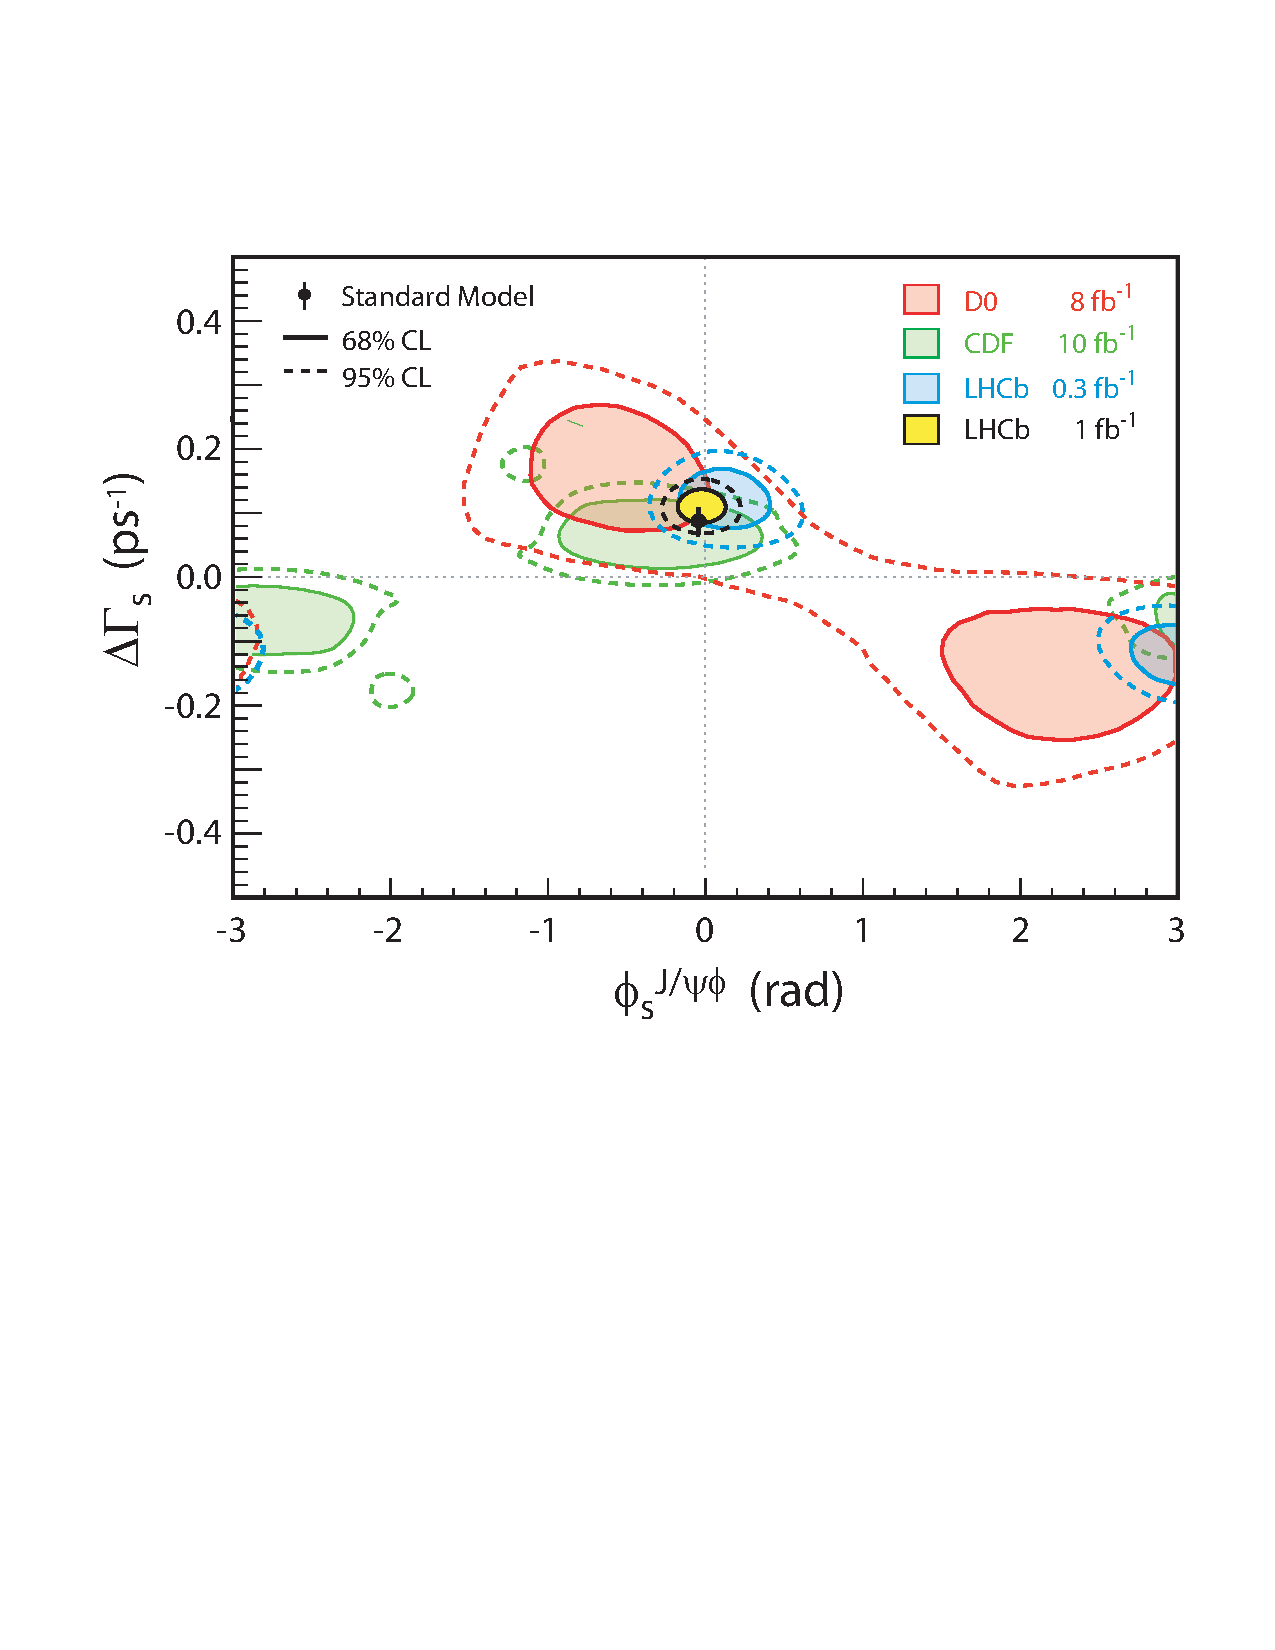
\includegraphics[scale=0.65,bb=50 300 580 700,clip=true]{Roger-plot}
    \vspace*{-1.0cm}
  \end{center}
  \caption{
    \small %captions should be a little bit smaller than main text
    Comparison of our result to those from other experiments.
    Note that the style of this figure differs slightly from that of Figure~\ref{fig:example}}
  \label{fig:roger}
\end{figure}

\clearpage


\addcontentsline{toc}{section}{References}
%\setboolean{inbibliography}{true}
\bibliographystyle{LHCb}
\bibliography{main,standard,LHCb-PAPER,LHCb-CONF,LHCb-DP,LHCb-TDR}
 
 
\newpage
% ===============================================================================
% Purpose: example of authorlist for LHCb template
% Author:
% Created on: 2009-09-24
% ===============================================================================

%\documentclass[a4paper]{article}
%\setlength{\oddsidemargin}{0cm}
%\setlength{\evensidemargin}{0cm}
%\setlength{\textwidth}{16.5cm}
%\setlength{\parindent}{0cm}
%\begin{document}
\centerline{\large\normalfont\bfseries LHCb collaboration}
\begin{flushleft}
\small
%-- LHCb Authorlist, Example typesetting
%-- 
A.~N.~Other$^{1}$.\bigskip\newline{\it
\footnotesize
$ ^{1}$University of nowhere\\
}
%-- 
%-- 
\end{flushleft}
%\end{document}




The author list for journal publications is generated from the
Membership Database shortly after 'approval to go to paper' has been
given.  It will be sent to you by email shortly after a paper number
has been assigned.  The author list should be included in the draft used for 
first and second circulation, to allow new members of the collaboration to verify
that they have been included correctly. Occasionally a misspelled
name is corrected, or associated institutions become full members.
Therefore an updated author list will be sent to you after the final
EB review of the paper.  In case line numbering doesn't work well
after including the authorlist, try moving the \verb!\bigskip! after
the last author to a separate line.


The authorship for Conference Reports should be ``The LHCb
collaboration'', with a footnote giving the name(s) of the contact
author(s), but without the full list of collaboration names.


The authorship for Figure Reports should be ``The LHCb
collaboration'', with no contact author and without the full list 
of collaboration names.


\end{document}
